% Options for packages loaded elsewhere
\PassOptionsToPackage{unicode}{hyperref}
\PassOptionsToPackage{hyphens}{url}
\documentclass[
]{book}
\usepackage{xcolor}
\usepackage{amsmath,amssymb}
\setcounter{secnumdepth}{5}
\usepackage{iftex}
\ifPDFTeX
  \usepackage[T1]{fontenc}
  \usepackage[utf8]{inputenc}
  \usepackage{textcomp} % provide euro and other symbols
\else % if luatex or xetex
  \usepackage{unicode-math} % this also loads fontspec
  \defaultfontfeatures{Scale=MatchLowercase}
  \defaultfontfeatures[\rmfamily]{Ligatures=TeX,Scale=1}
\fi
\usepackage{lmodern}
\ifPDFTeX\else
  % xetex/luatex font selection
\fi
% Use upquote if available, for straight quotes in verbatim environments
\IfFileExists{upquote.sty}{\usepackage{upquote}}{}
\IfFileExists{microtype.sty}{% use microtype if available
  \usepackage[]{microtype}
  \UseMicrotypeSet[protrusion]{basicmath} % disable protrusion for tt fonts
}{}
\makeatletter
\@ifundefined{KOMAClassName}{% if non-KOMA class
  \IfFileExists{parskip.sty}{%
    \usepackage{parskip}
  }{% else
    \setlength{\parindent}{0pt}
    \setlength{\parskip}{6pt plus 2pt minus 1pt}}
}{% if KOMA class
  \KOMAoptions{parskip=half}}
\makeatother
\usepackage{longtable,booktabs,array}
\usepackage{calc} % for calculating minipage widths
% Correct order of tables after \paragraph or \subparagraph
\usepackage{etoolbox}
\makeatletter
\patchcmd\longtable{\par}{\if@noskipsec\mbox{}\fi\par}{}{}
\makeatother
% Allow footnotes in longtable head/foot
\IfFileExists{footnotehyper.sty}{\usepackage{footnotehyper}}{\usepackage{footnote}}
\makesavenoteenv{longtable}
\usepackage{graphicx}
\makeatletter
\newsavebox\pandoc@box
\newcommand*\pandocbounded[1]{% scales image to fit in text height/width
  \sbox\pandoc@box{#1}%
  \Gscale@div\@tempa{\textheight}{\dimexpr\ht\pandoc@box+\dp\pandoc@box\relax}%
  \Gscale@div\@tempb{\linewidth}{\wd\pandoc@box}%
  \ifdim\@tempb\p@<\@tempa\p@\let\@tempa\@tempb\fi% select the smaller of both
  \ifdim\@tempa\p@<\p@\scalebox{\@tempa}{\usebox\pandoc@box}%
  \else\usebox{\pandoc@box}%
  \fi%
}
% Set default figure placement to htbp
\def\fps@figure{htbp}
\makeatother
\ifLuaTeX
  \usepackage{luacolor}
  \usepackage[soul]{lua-ul}
\else
  \usepackage{soul}
\fi
\setlength{\emergencystretch}{3em} % prevent overfull lines
\providecommand{\tightlist}{%
  \setlength{\itemsep}{0pt}\setlength{\parskip}{0pt}}
\usepackage[]{natbib}
\bibliographystyle{plainnat}
\usepackage{booktabs}

\usepackage{color}
\usepackage{framed}
\setlength{\fboxsep}{.8em}

% These colours were manually entered, they shouldn't matter unless you want pdf output

\newenvironment{redbox}{
  \definecolor{shadecolor}{RGB}{243, 154, 157}
  \color{white}
  \begin{shaded}}
 {\end{shaded}}

\newenvironment{bluebox}{
  \definecolor{shadecolor}{RGB}{172, 210, 237}
  \color{white}
  \begin{shaded}}
 {\end{shaded}}

\newenvironment{greenbox}{
  \definecolor{shadecolor}{RGB}{141, 181, 128}
  \color{white}
  \begin{shaded}}
 {\end{shaded}}
\usepackage{bookmark}
\IfFileExists{xurl.sty}{\usepackage{xurl}}{} % add URL line breaks if available
\urlstyle{same}
\hypersetup{
  pdftitle={Infectious Disease Genomic Epidemiology 2023},
  pdfauthor={Faculty: William Hsiao, Aaron Petkau, Jared Simpson, Fiona Brinkman, Finlay Maguire, Guillaume Bourque, Gary Van Domselaar, Ed Taboada, Emma Griffiths, Andrew McArthur, Michelle Brazas, Rhiannon Cameron, Karyn Mukiri, Miguel Prieto, Jimmy Liu, Jalees Nasir, Madeline McCarthy, Charlie Barclay, Nia Hughes, and Zhibin Lu},
  hidelinks,
  pdfcreator={LaTeX via pandoc}}

\title{Infectious Disease Genomic Epidemiology 2023}
\author{Faculty: William Hsiao, Aaron Petkau, Jared Simpson, Fiona Brinkman, Finlay Maguire, Guillaume Bourque, Gary Van Domselaar, Ed Taboada, Emma Griffiths, Andrew McArthur, Michelle Brazas, Rhiannon Cameron, Karyn Mukiri, Miguel Prieto, Jimmy Liu, Jalees Nasir, Madeline McCarthy, Charlie Barclay, Nia Hughes, and Zhibin Lu}
\date{April 18, 2023 - April 21, 2023}

\begin{document}
\maketitle

{
\setcounter{tocdepth}{1}
\tableofcontents
}
\part{Introduction}\label{part-introduction}

\chapter{Workshop Info}\label{workshop-info}

Welcome to the 2023 Infectious Disease Genomic Epidemiology Canadian Bioinformatics Workshop webpage!

\section{Class Photo}\label{class-photo}

\section{Schedule}\label{schedule}

\begin{longtable}[]{@{}
  >{\centering\arraybackslash}p{(\linewidth - 14\tabcolsep) * \real{0.0407}}
  >{\centering\arraybackslash}p{(\linewidth - 14\tabcolsep) * \real{0.2112}}
  >{\centering\arraybackslash}p{(\linewidth - 14\tabcolsep) * \real{0.0407}}
  >{\centering\arraybackslash}p{(\linewidth - 14\tabcolsep) * \real{0.2239}}
  >{\centering\arraybackslash}p{(\linewidth - 14\tabcolsep) * \real{0.0407}}
  >{\centering\arraybackslash}p{(\linewidth - 14\tabcolsep) * \real{0.1858}}
  >{\centering\arraybackslash}p{(\linewidth - 14\tabcolsep) * \real{0.0407}}
  >{\centering\arraybackslash}p{(\linewidth - 14\tabcolsep) * \real{0.2163}}@{}}
\toprule\noalign{}
\begin{minipage}[b]{\linewidth}\centering
\end{minipage} & \begin{minipage}[b]{\linewidth}\centering
\textbf{April 18}
\end{minipage} & \begin{minipage}[b]{\linewidth}\centering
\end{minipage} & \begin{minipage}[b]{\linewidth}\centering
\textbf{April 19}
\end{minipage} & \begin{minipage}[b]{\linewidth}\centering
\end{minipage} & \begin{minipage}[b]{\linewidth}\centering
\textbf{April 20}
\end{minipage} & \begin{minipage}[b]{\linewidth}\centering
\end{minipage} & \begin{minipage}[b]{\linewidth}\centering
\textbf{April 21}
\end{minipage} \\
\midrule\noalign{}
\endhead
\bottomrule\noalign{}
\endlastfoot
Time (EDT) & Module & Time (EDT) & Module & Time (EDT) & Module & Time (EDT) & Module \\
09:45 & Virtual Arrivals & 09:45 & Virtual Arrivals, Day 1 Check-in & 09:45 & Virtual Arrivals, Day 2 Check-in & 09:45 & Virtual Arrivals, Day 3 Check-in \\
10:00 & Virtual Welcome (Nia Hughes) & 10:00 & Module 4: Viral Pathogen Genomic Analysis - Single Nucleotide Variants (Jared Simpson) & 10:00 & Module 6: Antimicrobial Resistant Gene (AMR) Analysis (Andrew McArthur) & 10:00 & Module 8: Emerging Pathogen Detection and Identification (Aaron Petkau) \\
10:30 & Module 1: Introduction to Genomic Epidemiology (William Hsiao) & 11:00 & Break (30 mins) & 11:00 & Break (30 mins) & 11:00 & Break (30 mins) \\
11:30 & Break (30 mins) & 11:30 & Module 4 Lab (Jared Simpson) & 11:30 & Module 6 Lab (Andrew McArthur) & 11:30 & Module 8 Lab (Aaron Petkau) \\
12:00 & Module 2: Phylogenetic Analysis (Fiona Brinkman) & 13:30 & Break (1 hr) & 13:30 & Break (1 hr) & 13:30 & Break (1 hr) \\
13:00 & AWS setup (Zhibin Lu) & 14:30 & Module 5: Bacterial Pathogen Genomic Analysis (Ed Taboada) & 14:30 & Module 7: Phylodynamics and Transmission Dynamics (Finlay Maguire) & 14:30 & Keynote Lecture (Samira Mubareka) \\
13:30 & Break (1 hr) & 15:30 & Break (30 mins) & 15:30 & Break (30 mins) & 15:30 & Break (30 mins) \\
14:30 & Module 3: Data Curation and Data Sharing (Emma Griffiths) & 16:00 & Module 5 Lab (Ed Taboada) & 16:00 & Module 7 Lab (Finlay Maguire) & 16:00 & Module 9: Mobile Genetic Elements and Environmental Microbiome (Gary Van Domselaar) \\
15:30 & Break (30 mins) & 18:00 & End of Day 2 & 18:00 & Class Photo & 17:00 & Module 9 Lab (Gary Van Domselaar) \\
16:00 & Module 3 Lab (Emma Griffiths) & 18:00 & (Optional) Networking Virtual Social via Spatial Chat (until 19:00) & 18:15 & End of Day 3 & 18:00 & Survey \& Closing Remarks \\
18:00 & End of Day 1 & & & & & 18:30 & End of Workshop \\
18:00 & (Optional) Virtual Q\&A on how to sustain skills beyond the workshop (until 18:30) & & & & & & \\
\end{longtable}

\section{Pre-work}\label{pre-work}

\href{https://docs.google.com/forms/d/e/1FAIpQLSdPFL6pblmNLTYBnahXSiPIvlU8rXd21Hf07yu320Jgd6jjNg/viewform}{You can find your pre-work here.}

\chapter{Meet Your Faculty}\label{meet-your-faculty}

\subsubsection{William Hsiao}\label{william-hsiao}

\begin{quote}
Associate Professor
Faculty of Health Sciences, Simon Fraser University
Vancouver, BC, CA

--- \href{mailto:wwhsiao@sfu.ca}{\nolinkurl{wwhsiao@sfu.ca}}
\url{www.cidgoh.ca}
\end{quote}

William Hsiao is a public health infectious disease researcher with a background in microbial
genomics and bioinformatics. He is an associate professor in the Faculty of Health Sciences at
Simon Fraser University and an affiliated researcher at BCCDC Public Health Laboratory and at
Canada's Michael Smith Genome Sciences Centre. Will leads an interdisciplinary group of
researchers interested in solving practical public health and animal health problems through a
One Health lens at the Centre for Infectious Disease Genomics and One Health.

\subsubsection{Aaron Petkau}\label{aaron-petkau}

\begin{quote}
Head of Bioinformatics Pipeline Development
Science Technology Cores and Services
National Microbiology Laboratory
Public Health Agency of Canada
Winnipeg, MB, CA

--- \href{mailto:aaron.petkau@phac-aspc.gc.ca}{\nolinkurl{aaron.petkau@phac-aspc.gc.ca}}
\end{quote}

William Hsiao is a public health infectious disease researcher with a background in microbial
genomics and bioinformatics. He is an associate professor in the Faculty of Health Sciences at
Simon Fraser University and an affiliated researcher at BCCDC Public Health Laboratory and at
Canada's Michael Smith Genome Sciences Centre. Will leads an interdisciplinary group of
researchers interested in solving practical public health and animal health problems through a
One Health lens at the Centre for Infectious Disease Genomics and One Health.

\subsubsection{Jared Simpson}\label{jared-simpson}

\begin{quote}
Principal Investigator, Ontario Institute for Cancer Research
Assistant Prof.~Department of Computer Science, University of Toronto
Vancouver, BC, CA

---\url{https://simpsonlab.github.io/}
\end{quote}

Dr.~Simpson develops algorithms and software for the analysis of
high-throughput sequencing data. He is interested in de novo assembly and the detection of
sequence variation in individuals, cancers and populations, with a focus on long read
sequencing technologies. Dr.~Simpson developed the ABYSS, SGA and nanopolish software
packages.

\subsubsection{Fiona Brinkman}\label{fiona-brinkman}

\begin{quote}
Distinguished Professor, FRSC, Department of Molecular Biology and Biochemistry
Associate Member, School of Computing Science and Faculty of Health Sciences
Simon Fraser University
Burnaby, BC, CA

--- \href{mailto:brinkman@sfu.ca}{\nolinkurl{brinkman@sfu.ca}}
\url{https://www.brinkmanlab.ca/}
\end{quote}

Dr.~Brinkman is developing bioinformatic resources to better track infectious diseases using
genomic data, and improve prediction of new vaccine/drug targets. Her primary aim is to
develop more sustainable, integrated approaches for infectious disease control, however she is
also applying her methods to aid allergy, child health, and environmental research.

\subsubsection{Finlay Maguire}\label{finlay-maguire}

\begin{quote}
Assistant Professor
Faculty of Computer Science and Department of Community Health \& Epidemiology
Dalhousie University
Halifax, NS, CA

--- \href{mailto:finlay.maguire@dal.ca}{\nolinkurl{finlay.maguire@dal.ca}}
\url{finlaymagui.re}
\end{quote}

Finlay Maguire is a data scientist whose work centers on leveraging data in innovative ways to
answer questions related to applied health and social issues. This includes developing
bioinformatics methods to more effectively use genomic data to mitigate infectious diseases and
broad interdisciplinary collaborations in areas such as refugee healthcare provision and online
radicalisation. They are an active contributor to the national and international public health
responses to the COVID-19 pandemic and act as a genomic epidemiology advisor for
Sunnybrook's Shared Hospital Laboratory.

\subsubsection{Guillaume Bourque}\label{guillaume-bourque}

\begin{quote}
Professor, McGill University
Director of Bioinformatics, Genome Quebec Innovation Centre
Director, Canadian Centre of Computational Genomics
Director, McGill initiative for Computational Medicine
\end{quote}

Dr.~Bourque's research interests are in comparative and functional genomics with a special
emphasis on applications of next-generation sequencing technologies. His lab develops
advanced tools and scalable computational infrastructure to enable large-scale applied research
projects.

\subsubsection{Gary Van Domselaar}\label{gary-van-domselaar}

\begin{quote}
Chief Bioinformatics Scientist
National Microbiology Laboratory
Public Health Agency of Canada
Winnipeg, MB, CA

--- \href{mailto:gary.vandomselaar@phac-aspc.gc.ca}{\nolinkurl{gary.vandomselaar@phac-aspc.gc.ca}}
\end{quote}

Dr.~Gary Van Domselaar, PhD (University of Alberta, 2003) is the Chief Bioinformatics Scientist at
the National Microbiology Laboratory in Winnipeg Canada and Associate Professor in the
Department of Medical Microbiology and Infectious Diseases at the University of Manitoba. Dr.~Van
Domselaar's lab develops bioinformatics methods and pipelines to understand, track, and control
circulating infectious diseases in Canada and globally. His research and development activities span
metagenomics, infectious disease genomic epidemiology, genome annotation, population structure
analysis, and microbial genome wide association studies. His lab contributes to large-scale national
and international genomics and bioinformatics efforts, including the Bioinformatics Workgroup of the
Canadian Genomics Research and Development Initiative Interdepartmental Project on
Antimicrobial Resistance, the Integrated Rapid Infectious Disease Analysis (IRIDA) project to
develop an integrated computational platform for infectious disease outbreak investigations, the
Canadian COVID-19 genomics network (CanCOGeN), and the Canadian Public Health Laboratory
Network COVID-19 Genomics Program. Dr.~Van Domselaar serves on a number of national and
international scientific advisory groups, including the US Centers for Disease Control, the Global
Coalition for Science and Regulatory Research, and PHA4GE.

\subsubsection{Ed Taboada}\label{ed-taboada}

\begin{quote}
Research Scientist
Genomic Epidemiology Research Unit
Division of Enteric Diseases
National Microbiology Laboratory
Public Health Agency of Canada
Winnipeg, MB, CA

--- \href{mailto:eduardo.taboada@phac-aspc.gc.ca}{\nolinkurl{eduardo.taboada@phac-aspc.gc.ca}}
\end{quote}

Eduardo Taboada is a research scientist in the Division of Enteric Diseases at the NML. Since
obtaining his PhD in molecular genetics at the Department of Biology, University of Ottawa in
1999, he has applied his expertise in molecular biology and population genetics towards the
development of comparative genomics and bioinformatics-based tools for studying various
aspects of the biology, ecology, and epidemiology of bacterial food- and waterborne pathogens,
with a focus on Campylobacter, Salmonella, and E. coli. Over these past two decades, Ed has
led or participated in several projects funded by Genome Canada and the federal government's
Genomics Research and Development Initiative. His current research focus is on developing
quantitative tools for integrated genomic and epidemiologic analysis and the application of
analytical epidemiology approaches to genomic datasets.

\subsubsection{Emma Griffiths}\label{emma-griffiths}

\begin{quote}
Emma Griffiths
Research Associate
Faculty of Health Sciences, Simon Fraser University
Vancouver, BC, Canada

--- \href{mailto:emma_griffiths@sfu.ca}{\nolinkurl{emma\_griffiths@sfu.ca}}
\end{quote}

Emma Griffiths is a research associate at the Centre for Infectious Disease Genomics and One
Health (CIDGOH) in the Faculty of Health Sciences at Simon Fraser University in Vancouver,
Canada. Her work focuses on developing and implementing ontologies and data standards for
public health and food safety genomics to help improve data harmonization and integration. She
is a member of the Standards Council of Canada and leads the Public Health Alliance for
Genomic Epidemiology (PHA4GE) Data Structures Working Group.

\subsubsection{Andrew McArthur}\label{andrew-mcarthur}

\begin{quote}
Professor and Director BDC Program
Biochemistry and Biomedical Sciences
McMaster University
Hamilton, ON, CA
\end{quote}

Dr.~McArthur is a Professor and David Braley Chair in Computational Biology at McMaster
University. Dr.~McArthur has had a career in the United States and Canada, including
NIH-funded positions at the Marine Biological Laboratory and Brown University, where he led
the genome assembly of the diarrheal pathogen Giardia intestinalis, plus 10 years of experience
in the private sector. Dr.~McArthur's research team focuses on building tools, databases, and
algorithms for the genomic surveillance of infectious pathogens. He and his team developed the
Comprehensive Antibiotic Resistance Database (card.mcmaster.ca) and the SARS-CoV-2
Illumina GeNome Assembly Line software platform.

\subsubsection{Michelle Brazas}\label{michelle-brazas}

\begin{quote}
Acting Scientific Director
Canadian Bioinformatics Workshops (CBW)
Toronto, ON, CA

--- \href{mailto:support@bioinformatics.ca}{\nolinkurl{support@bioinformatics.ca}}
\end{quote}

Dr.~Michelle Brazas is the Associate Director for Adaptive Oncology at the Ontario Institute for
Cancer Research (OICR), and acting Scientific Director at Bioinformatics.ca. Previously, Dr.
Brazas was the Program Manager for Bioinformatics.ca and a faculty member in Biotechnology
at BCIT. Michelle co-founded and runs the Toronto Bioinformatics User Group (TorBUG) now in
its 11th season, and plays an active role in the International Society of Computational Biology
where she sits on the Board of Directors and Executive Board.

\subsubsection{Rhiannon Cameron}\label{rhiannon-cameron}

\begin{quote}
PhD Graduate Student Researcher
Faculty of Health Sciences, Simon Fraser University
Vancouver, BC, CA

--- \href{mailto:rcameron@sfu.ca}{\nolinkurl{rcameron@sfu.ca}}
\url{https://cmrn-rhi.github.io/}
\end{quote}

Rhiannon completed her Bachelor of Science in Microbiology in 2019 and is currently a PhD
student in the Faculty of Health Sciences at SFU under the supervision of Dr.~Hsiao at the
Centre for Infectious Disease Genomics and One Health (CIDGOH). Her work focuses on
ontology curation and development for outbreak investigation and surveillance of SARS-CoV-2
for the Canadian COVID-19 Genomics Network (CanCOGeN) and food-borne pathogen risk
assessment modeling for the Canadian Antimicrobial Resistance Genomics Research and
Development Initiative (AMR-GRDI), and developing ontology/metadata-curation training
resources. In her spare time, Rhiannon volunteers with the Vancouver Bioinformatics User
Group and the Neil Squire Society Computer Comforts program.

\subsubsection{Karyn Mukiri}\label{karyn-mukiri}

\begin{quote}
PhD Graduate Student Researcher
Faculty of Health Sciences, McMaster University
Department of Biochemistry and Biomedical Sciences
Hamilton, ON, CA

--- \href{mailto:mukirikm@mcmaster.ca}{\nolinkurl{mukirikm@mcmaster.ca}}
\end{quote}

Karyn is a second-year PhD student under the supervision of Dr.~Andrew McArthur where her
main research focus is on the development of predictive genomic annotation algorithms to
increase antibiotic resistance surveillance by the Resistance Gene Identifier. She is also a
McMaster alum, having completed her undergraduate degree in Biotechnology under the
Faculty of Engineering. Although the bulk of her work focuses on more algorithmic problems,
her current research efforts are in helping pinpoint instances of miscuration within the
Comprehensive Antibiotic Resistance Database.

\subsubsection{Miguel Prieto}\label{miguel-prieto}

\begin{quote}
PhD Graduate Student Researcher
Simon Fraser University
Faculty of Health Sciences
Vancouver, BC, CA

--- \href{mailto:mprietog@sfu.ca}{\nolinkurl{mprietog@sfu.ca}}
\end{quote}

Miguel is a first year PhD student studying the impact of human infectious diseases and the role
of the microbiome in humans. Particularly, he aims to use machine learning and metagenomic
analysis to predict poor outcomes in chronic respiratory diseases. Miguel is a Medical Doctor
from the Universidad del Valle in Colombia and has worked as a researcher and project
coordinator on translational studies of neglected tropical diseases like leishmaniasis. Before
coming to SFU, he completed a Master of Experimental Medicine at UBC exploring blood-based
gene expression biomarkers of nontuberculous mycobacterial infections in patients with cystic
fibrosis.

\subsubsection{Jimmy Liu}\label{jimmy-liu}

\begin{quote}
PhD Graduate Student Researcher
Simon Fraser University
Department of Molecular Biology and Biochemistry
Burnaby, BC, CA

--- \href{mailto:ccl40@sfu.ca}{\nolinkurl{ccl40@sfu.ca}}
\end{quote}

Jimmy Liu completed his BSc. in Biochemistry at the University of British Columbia in 2019.
During his undergraduate study, he worked as a lab technologist at the JC Wilt Infectious
Diseases Research Centre where he developed passion for infectious disease genomics.
Inspired by the widespread adoption of genomic sequencing to inform decison making, he
decided to pursue further training in bioinformatics and genomic epidemiology by joining Dr.
William Hsiao's group at the Simon Fraser University as a Ph.D.~trainee. His thesis research
involves the joint application of machine learning, graph structures, and sequence alignment
algorithms to characterize the pan-genome evolution of Salmonella enterica. The discoveries
from his pan-genome analyses will drive the refinement of existing typing methods for disease
reporting and outbreak detection.

\subsubsection{Jalees Nasir}\label{jalees-nasir}

\begin{quote}
PhD Graduate Student Researcher
McMaster University
Department of Biochemistry and Biomedical Sciences
Hamilton, ON, CA

--- \href{mailto:nasirja@mcmaster.ca}{\nolinkurl{nasirja@mcmaster.ca}}
\end{quote}

Jalees Nasir is a Ph.D.~Candidate in the McArthur Laboratory at McMaster University. His work
focuses on developing molecular epidemiological tools for the surveillance of respiratory viral
infections, including SARS-CoV-2. These tools primarily come in the form of molecular assays
for target enrichment, including bait capture. However, with the advent of the COVID-19
pandemic, he has also developed software for processing sequencing data (SARS-CoV-2
Illumina GeNome Assembly Line; SIGNAL) to contribute to ongoing surveillance efforts.

\subsubsection{Madeline McCarthy}\label{madeline-mccarthy}

\begin{quote}
PhD Graduate Student Researcher
McMaster University
Department of Biochemistry and Biomedical Sciences
Hamilton, ON, CA

--- \href{mailto:mccarm15@mcmaster.ca}{\nolinkurl{mccarm15@mcmaster.ca}}
\end{quote}

Madeline is a PhD Candidate in the McArthur Lab at McMaster University. Her work focuses on
the development of targeted, cost-effective methods for culture-free outbreak detection and
surveillance of bacterial pathogens. In addition to whole genome capture, she is testing the
feasibility of targeted, culture-free plasmid recovery using bait capture and long-read
sequencing. Prior to her PhD, she completed a MSc in microbiology at the University of
Saskatchewan where she studied E. coli outbreaks in broiler chickens before hanging up her
pipettes and switching to bioinformatics.

\subsubsection{Charlie Barclay}\label{charlie-barclay}

\begin{quote}
MSc Graduate Student Researcher
University of British Columbia
Department of Physics and Astronomy
Vancouver, BC, CA

--- \href{mailto:cbarcl01@mail.ubc.ca}{\nolinkurl{cbarcl01@mail.ubc.ca}}
\end{quote}

Charlie completed her Masters in Marine Biology from the University of Southampton in 2013
and then spent 5 years working as a Data Manager at the Natural History Museum (NHM) in
London, during which she became involved in the Darwin Tree of Life project, standardizing
data at capture which led her to retrain in Bioinformatics. Charlie is currently working on the de
novo genome assembly of a comb jelly Mnemiopsis leidyi and how genomic insights of this
early branching metazoan can help us uncover mechanisms into cell differentiation and
multicellularity. Recently she has furthered her interest in FAIR data and ontologies through an
internship in Centre for Infectious Disease Genomics and One Health (CIDGOH).

\subsubsection{Nia Hughes}\label{nia-hughes}

\begin{quote}
Program Manager, Bioinformatics.ca
Ontario Institute for Cancer Research
Toronto, ON, CA

--- \href{mailto:nia.hughes@oicr.on.ca}{\nolinkurl{nia.hughes@oicr.on.ca}}
\end{quote}

Nia is the Program Manager for Bioinformatics.ca, where she coordinates the Canadian
Bioinformatics Workshop Series. Prior to starting at OICR, she completed her M.Sc. in
Bioinformatics from the University of Guelph in 2020 before working there as a bioinformatician
studying epigenetic and transcriptomic patterns across maize varieties.

\subsubsection{Zhibin Lu}\label{zhibin-lu}

\begin{quote}
HPC and Bioinformatics Services Manager at Princess Margaret
Cancer Centre, University Health Network
Bioinformatics and HPC Core, UHN
Toronto, ON, CA

--- \href{mailto:zhibin@gmail.com}{\nolinkurl{zhibin@gmail.com}}
\url{https://bhpc.uhnresearch.ca/}
\end{quote}

Zhibin Lu is a senior manager at University Health Network Digital. He is responsible for UHN
HPC operations and scientific software. He manages two HPC clusters at UHN, including
system administration, user management, and maintenance of bioinformatics tools for
HPC4health. He is also skilled in Next-Gen sequence data analysis and has developed and
maintained bioinformatics pipelines at the Bioinformatics and HPC Core. He is a member of the
Digital Research Alliance of Canada Bioinformatics National Team and Scheduling National
Team.

\chapter{Data and Compute Setup}\label{data-and-compute-setup}

\subsubsection{Course Data Downloads}\label{course-data-downloads}

Some of these files are quite large. If you have issues downloading them, contact us at \href{mailto:support@bioinformatics.ca}{\nolinkurl{support@bioinformatics.ca}}.

\begin{itemize}
\tightlist
\item
  \href{}{Unix}
\item
  \href{}{Module 4}
\item
  \href{}{Module 5}
\item
  \href{}{Module 6}
\item
  \href{}{Module 7}
\item
  \href{}{Module 8}
\item
  \href{}{Module 9}
\end{itemize}

\subsubsection{Compute setup}\label{compute-setup}

\paragraph{AWS Module}\label{aws-module}

Please follow the \href{https://bioinformaticsdotca.github.io/AWS_setup}{instructions} to log into your AWS instance.
The content for our AWS/Unix review session on April 17th can be found \href{https://bioinformaticsdotca.github.io/AWS_IDE23}{here}.
The schedule for this session can be found \href{https://bioinformaticsdotca.github.io/AWS_IDE23_Schedule}{here}.

\paragraph{AMI}\label{ami}

We have made our AWS AMI (Amazon Machine Image) publicly available. To launch your own instance, follow the instructions provided by Amazon on \href{https://repost.aws/knowledge-center/launch-instance-custom-ami}{how to launch an EC2 instance from a custom Amazon Machine Image}. Please note that you will need an AWS account to proceed, and that you will need to upload the CourseData files yourself.

Here are the details of the AMI:

\begin{itemize}
\tightlist
\item
  AWS Region: us-east-1 (N. Virgina)
\item
  AMI type: public image
\item
  AMI name: CBW\_230416
\item
  AMI ID: ami-0b905fa1d1d233a17
\end{itemize}

If you want to create and activate a new AWS account, please follow the \href{https://aws.amazon.com/premiumsupport/knowledge-center/create-and-activate-aws-account/}{instructions} provided by Amazon.

\paragraph{Software}\label{software}

For information on installing the necessary tools, please visit:

\href{https://bioinformaticsdotca.github.io/IDE_2023_tools}{Tool Installation}

\part{Modules}\label{part-modules}

\chapter{Module 1: Introduction to Genomic Epidemiology}\label{module-1-introduction-to-genomic-epidemiology}

\section{Lecture}\label{lecture}

\chapter{Module 2: Phylogenetic Analysis}\label{module-2-phylogenetic-analysis}

\section{Lecture}\label{lecture-1}

\section{AWS Setup}\label{aws-setup}

You can find the instructions \href{https://bioinformaticsdotca.github.io/AWS_setup}{here}.

\chapter{Module 3: Data Curation and Data Sharing}\label{module-3-data-curation-and-data-sharing}

\section{Lecture}\label{lecture-2}

\section{Lab}\label{lab}

Congratulations! You have completed Lab 3!

\chapter{Module 4: Viral Pathogen Genomic Analysis - Single Nucleotide Variants}\label{module-4-viral-pathogen-genomic-analysis---single-nucleotide-variants}

\section{Lecture}\label{lecture-3}

\section{Lab}\label{lab-1}

\subsection{Virus Short-Read Genome Assembly and Variant Analysis}\label{virus-short-read-genome-assembly-and-variant-analysis}

\emph{By Jared Simpson and Jalees Nasir}

\subsubsection{Introduction}\label{introduction}

In this lab we will perform reference-based analysis of Severe Acute Respiratory Syndrome Coronavirus 2 (SARS-CoV-2) short-read sequencing data. You will be guided through the analysis workflow and subsequent exploration of the data and quality control results. At the end of the lab you will know:

\begin{enumerate}
\def\labelenumi{\arabic{enumi}.}
\tightlist
\item
  How to analyze amplicon sequencing data from the Illumina sequencing instrument
\item
  How to assess the quality of a sequenced sample
\item
  How to assess single nucleotide polymorphisms (SNPs) for SARS-CoV-2 variant calls
\item
  How to view the evolutionary changes of SARS-CoV-2 and interpret differences between lineages belonging to variants of concern (i.e., Alpha vs.~Delta variants)
\end{enumerate}

\subsubsection{Datasets}\label{datasets}

In this lab we will use subset of data from the COVID-19 Genomics UK Consortium (COG-UK) to demonstrate analysis of SARS-CoV-2. This data set consists of short-read sequencing reads collected as part of the COVID-19 Pandemic response and will be a mix of different variants of concern (VOCs) up to the end of summer 2021. This would include predominantly Alpha (also known as PANGO lineage B.1.1.7; first designated December 2020) and Delta (also known as PANGO lineage B.1.617.2; first designated in May 2021) variants. We have provided publicly available Illumina short-reads and you will run SARS-CoV-2 Illumina GeNome Assembly Line (\texttt{SIGNAL}) with additional quality control and assessment using \texttt{ncov-tools}. Prior to the workshop the instructors downsampled the sequencing data from \textasciitilde10,000x coverage to \textasciitilde200x coverage to reduce the time it takes to run the analysis; however, running the pipelines use the exact same set of commands and the results you will obtain are comparable to assembling using the full dataset.

In the following instructions the commands you should run are shown in code blocks like so:

\begin{verbatim}
echo "Hello world"
\end{verbatim}

You can type these commands into your terminal, or copy and paste them.

\subsubsection{Data Download and Preparation}\label{data-download-and-preparation}

First, lets create and move to a directory that we'll use to organize our results:

\begin{verbatim}
mkdir -p workspace/module4
cd workspace/module4
\end{verbatim}

From within your \texttt{module4} directory, you can create a symlink which is a shortcut to where the raw sequencing data is stored:

\begin{verbatim}
### Current working directory: ~/workspace/module4

ln -s ~/CourseData/IDE_data/module4/cbw_demo_run/
\end{verbatim}

If you run \texttt{ls} you should see only one directory: \texttt{cbw\_demo\_run}.

You can view the contents of the cbw\_demo\_run directory using \texttt{ls}:

\begin{verbatim}
ls cbw_demo_run
\end{verbatim}

You should see 36 pairs of files. Each pair of files is the raw sequencing data for a single sample. The first half of the Illumina paired-end reads is stored in files ending in \texttt{\_R1.fastq.gz} and the second half in \texttt{\_R2.fastq.gz}. The samples are identified with accession numbers like \texttt{ERR5338522}, a unique identifier of a sample that has been deposited in a public database. You can view the contents of one of the data files by decompressing it and piping it to \texttt{head}:

\begin{verbatim}
zcat cbw_demo_run/ERR5338522_R1.fastq.gz | head
\end{verbatim}

Question: what do the different lines in a FASTQ file mean? If you can't figure it out ask an instructor or on slack!

\subsubsection{Running SIGNAL}\label{running-signal}

The analysis of SARS-CoV-2 sequencing data is complex and uses a number of different tools that are run sequentially in a pipeline. The pipeline we will use to analyze this data is called \texttt{SIGNAL}. First, we need to clone a copy of SIGNAL from github and then enter the directory this command creates:

\begin{verbatim}
git clone --recursive https://github.com/jaleezyy/covid-19-signal
cd covid-19-signal
\end{verbatim}

Ensure that your current working directory is within the \texttt{covid-19-signal} directory using \texttt{pwd}. Next, we need to switch to the version of SIGNAL that we will use for this workshop. This version tells SIGNAL that we have installed all of the software we used in a single conda environment:

\begin{verbatim}
git checkout single-conda
\end{verbatim}

Finally, we need to activate the conda environment containing the software SIGNAL requires, and create a symlink to the reference files SIGNAL needs. You can also review the SIGNAL help screen to see our options:

\begin{verbatim}
conda activate signalcovtools
ln -s ~/CourseData/IDE_data/module4/data/

### Current working directory: ~/workspace/module4/covid-19-signal

python signalexe.py -h
\end{verbatim}

The \texttt{data} directory you have linked should be found within \texttt{\textasciitilde{}/workspace/module4/covid-19-signal/data}.

In order to run SIGNAL, we first need to prepare two files: a configuration file, where all of our assembly parameters will be assigned, and a sample table, which will list the indivdual samples and the location of corresponding R1 and R2 FASTQs. Remember that our sequencing data is located one directory level up (i.e., \texttt{../cbw\_demo\_run/}). Generating the required files can all be done using the following command:

\begin{verbatim}
### Current working directory: ~/workspace/module4/covid-19-signal

python signalexe.py --directory ../cbw_demo_run --config-only
\end{verbatim}

The output should be as follows

If you run \texttt{ls} you should see \texttt{cbw\_demo\_run\_config.yaml} and \texttt{cbw\_demo\_run\_sample\_table.csv} files have been created. You can use \texttt{more} or \texttt{less} to examine the input files.

\subsubsection{Reference-based Assembly Using SIGNAL}\label{reference-based-assembly-using-signal}

Using our configuration file as input, we can begin our assembly of SARS-CoV-2 sequencing reads. Run the following:

\begin{verbatim}
python signalexe.py --configfile cbw_demo_run_config.yaml --quiet --cores 4 all postprocess
\end{verbatim}

This will take around 30-45 minutes to run, so is a good time for a short break.

\subsubsection{Quality Control and Assessment}\label{quality-control-and-assessment}

Now that SIGNAL is complete, we will run an additional step to generate some quality control results:

\begin{verbatim}
python signalexe.py --configfile cbw_demo_run_config.yaml --quiet --cores 4 ncov_tools
\end{verbatim}

\subsubsection{Coverage Analysis}\label{coverage-analysis}

We can now start exploring the results. First we will look at the depth of coverage to make sure that each viral genome was covered by enough sequencing reads to call an accurate consensus sequence.

Open your web browser and navigate to \texttt{http://xx.uhn-hpc.ca/module4/covid-19-signal/cbw\_demo\_run\_results\_dir/} where xx is the instance ID you were assigned. This directory stores the results of SIGNAL and ncov-tools. In the \texttt{ncov-tools-results/plots/} subdirectory you will find a file called \texttt{cbw\_demo\_run\_results\_dir\_depth\_by\_position.pdf}. Open this file.

This file contains plots of the coverage depth for each of the 36 samples we analyzed as shown below.

Explore the results and try to understand what the coverage patterns mean:

\begin{itemize}
\tightlist
\item
  What might have caused the sharp drop in coverage for sample \texttt{ERR6035561}?
\item
  What about the uneven coverage in sample \texttt{ERR5508530}?
\end{itemize}

As explained in the lecture, sequencing coverage is a critical factor for determining the \texttt{completeness} of the genome assembly. In the terminal, let's view the consensus sequence for sample \texttt{ERR5508530}:

\begin{verbatim}
<<<<<<< HEAD
cd ~/workspace/module4/covid-19-signal
=======
>>>>>>> main
less cbw_demo_run_results_dir/ERR5508530/freebayes/ERR5508530.consensus.fasta
\end{verbatim}

What do you see? The consensus sequences for other samples are in directories with similiar names, take a look at them. Can you draw any conclusions about the quality of the results?

ncov-tools creates a file that summarizes the genome completeness for every sample. Run this command in the terminal:

\begin{verbatim}
cut -f1,10,15 cbw_demo_run_results_dir/ncov-tools-results/qc_reports/cbw_demo_run_results_dir_summary_qc.tsv
\end{verbatim}

This command uses \texttt{cut} to find the metrics that we are interested in from the full QC results table. What is the completeness of \texttt{ERR5508530}? What about \texttt{ERR6035561}?

\subsubsection{Assessing SNP Calls}\label{assessing-snp-calls}

Now, using your browser open the file located at \texttt{ncov-tools-results/plots/cbw\_demo\_run\_results\_dir\_tree\_snps.pdf}.

This plot arranges the samples using a phylogenetic tree (shown on the left) so that samples with a similar sequence are grouped together. The panel on the right shows SNPs within each sample with respect to the MN908947.3 reference genome, where each colour represents a different base. Also shown on the plot are the pangolin-assigned lineages; B.1.1.7 is the alpha variant, AY.4 is delta. Notice that there are many SNPs in common between the alpha samples and a different set of SNPs in common between the delta samples. These SNPs are what define the different lineages.

Now, we're going to inspect the read-level evidence for some example SNPs. Open up IGV and using the first dropdown menu select the ``SARS-CoV-2'' genome. Now, click on the File menu and select ``Load from URL'' and paste in the path \texttt{http://xx.uhn-hpc.ca/module4/covid-19-signal/cbw\_demo\_run\_results\_dir/ERR5389257/core/ERR5389257\_viral\_reference.mapping.bam} again replacing xx with your instance ID. Once the file loads you will see the pattern of read coverage along the genome.

Paste the coordinates \texttt{NC\_045512.2:2,917-3,156} into the navigation bar. This region shows a single C\textgreater T SNP where every read supports the alternative allele (the red bars in the middle of the screen). Now, navigate to \texttt{NC\_045512.2:631-870}. In this case some reads have evidence for a C\textgreater T SNP but other reads have evidence for the reference allele at this position. Since this position is ambiguous the consensus genome will be marked with an ambiguity code. Going back to the mutations plot, look for the row corresponding to sample \texttt{ERR5389257}. Notice that it has a black bar in between two purple SNPs at the beginning of the genome - that is the ambiguous position that we are inspecting at IGV. Since this position is only ambiguous in \texttt{ERR5389257} we can't draw many conclusions from it - it could be due to low-level contamination, a PCR artificat, or heterogeneity within this sample.

You can view all of the variants for a sample by using \texttt{less} on their VCF files:

\begin{verbatim}
less cbw_demo_run_results_dir/ERR5389257/freebayes/ERR5389257.variants.norm.vcf
\end{verbatim}

Take a bit of time to look at other variants for this sample (or other samples!). If you find something interesting or unexpected tell the rest of the class in slack and we can discuss it as a group.

\subsubsection{Variant Consequence Prediction}\label{variant-consequence-prediction}

Once we have variant calls we can run a \texttt{mutation\ consequence\ predictor} to determine the protein-level changes. This is important as the identification of new variants relies on determining whether the mutations increase the fitness of the lineage, which is usually determined at the amino acid level. View this file in your terminal:

\begin{verbatim}
less cbw_demo_run_results_dir/ncov-tools-results/qc_annotation/ERR5389257_aa_table.tsv
\end{verbatim}

This file is a table of predicted amino acid changes for each protein. How many changes to the spike protein does this sample have? Let's compare that number to a different sample from another lineage. First, let's figure out the lineage of sample \texttt{ERR5389257}:

\begin{verbatim}
grep ERR5389257 cbw_demo_run_results_dir/lineage_assignments.tsv
\end{verbatim}

The file \texttt{lineage\_assignments.tsv} is produced by pangolin and by grepping (searching the file) for sample \texttt{ERR5389257} we can see that it is B.1.1.7 (Alpha). Look in the \texttt{lineage\_assignments.tsv} file to find the identifier for a delta sample, then use it's consequence prediction file to count the number of spike mutations. Is it more or less than \texttt{ERR5389257?} We probably wouldn't want to draw strong conclusions from the number of mutations as many will be neutral (or even deleterious) but this type of analysis - looking at mutation consequence - cross-referenced with other data (for example experimental fitness assays) is what goes into identifying VOCs.

Congratulations! You have completed Lab 4!

\chapter{Module 5: Bacterial Pathogen Genomic Analysis}\label{module-5-bacterial-pathogen-genomic-analysis}

\section{Lecture}\label{lecture-4}

\section{Lab}\label{lab-2}

The lab assignment is written in Rmarkdown (.Rmd) which means that the lab is intended to be run in RStudio IDE.

\subsection{Setup}\label{setup}

Before connecting to your RStudio instance, please perform the following steps:

\begin{enumerate}
\def\labelenumi{\arabic{enumi}.}
\tightlist
\item
  Log into your remote instance using ssh
\end{enumerate}

\begin{verbatim}
# replace xx with your student number
ssh -i CBW.pem xx.uhn-hpc.ca
\end{verbatim}

\begin{enumerate}
\def\labelenumi{\arabic{enumi}.}
\setcounter{enumi}{1}
\tightlist
\item
  Copy the lab materials from \texttt{CourseData} to \texttt{workspace/}
\end{enumerate}

\begin{verbatim}
cp -r  ~/CourseData/IDE_data/module5/ ~/workspace/
\end{verbatim}

\begin{enumerate}
\def\labelenumi{\arabic{enumi}.}
\setcounter{enumi}{2}
\tightlist
\item
  You should now find a directory called \texttt{module5} under \texttt{\textasciitilde{}/workspace/}. Use \texttt{ls} to list the file content in \texttt{\textasciitilde{}/workspace/module5} to verify that you have successfully copied all of the required files.
\end{enumerate}

\begin{verbatim}
ls ~/workspace/module5
\end{verbatim}

Expected output:

\pandocbounded{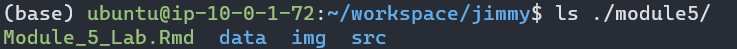
\includegraphics[keepaspectratio]{img/module_5_img_1.png}}
\#\#\#\# Launching RStudio

\begin{enumerate}
\def\labelenumi{\arabic{enumi}.}
\item
  Open a browser tab and navigate to \texttt{http://xx.uhn-hpc.ca:8080} (Remember to replace \texttt{xx} with your student number!)
\item
  Log in using the following credentials:
\end{enumerate}

\begin{itemize}
\tightlist
\item
  Username: ubuntu
\item
  Password will be provided in class
\end{itemize}

If logged in successfully, you should see the following graphical interface in your browser:

\pandocbounded{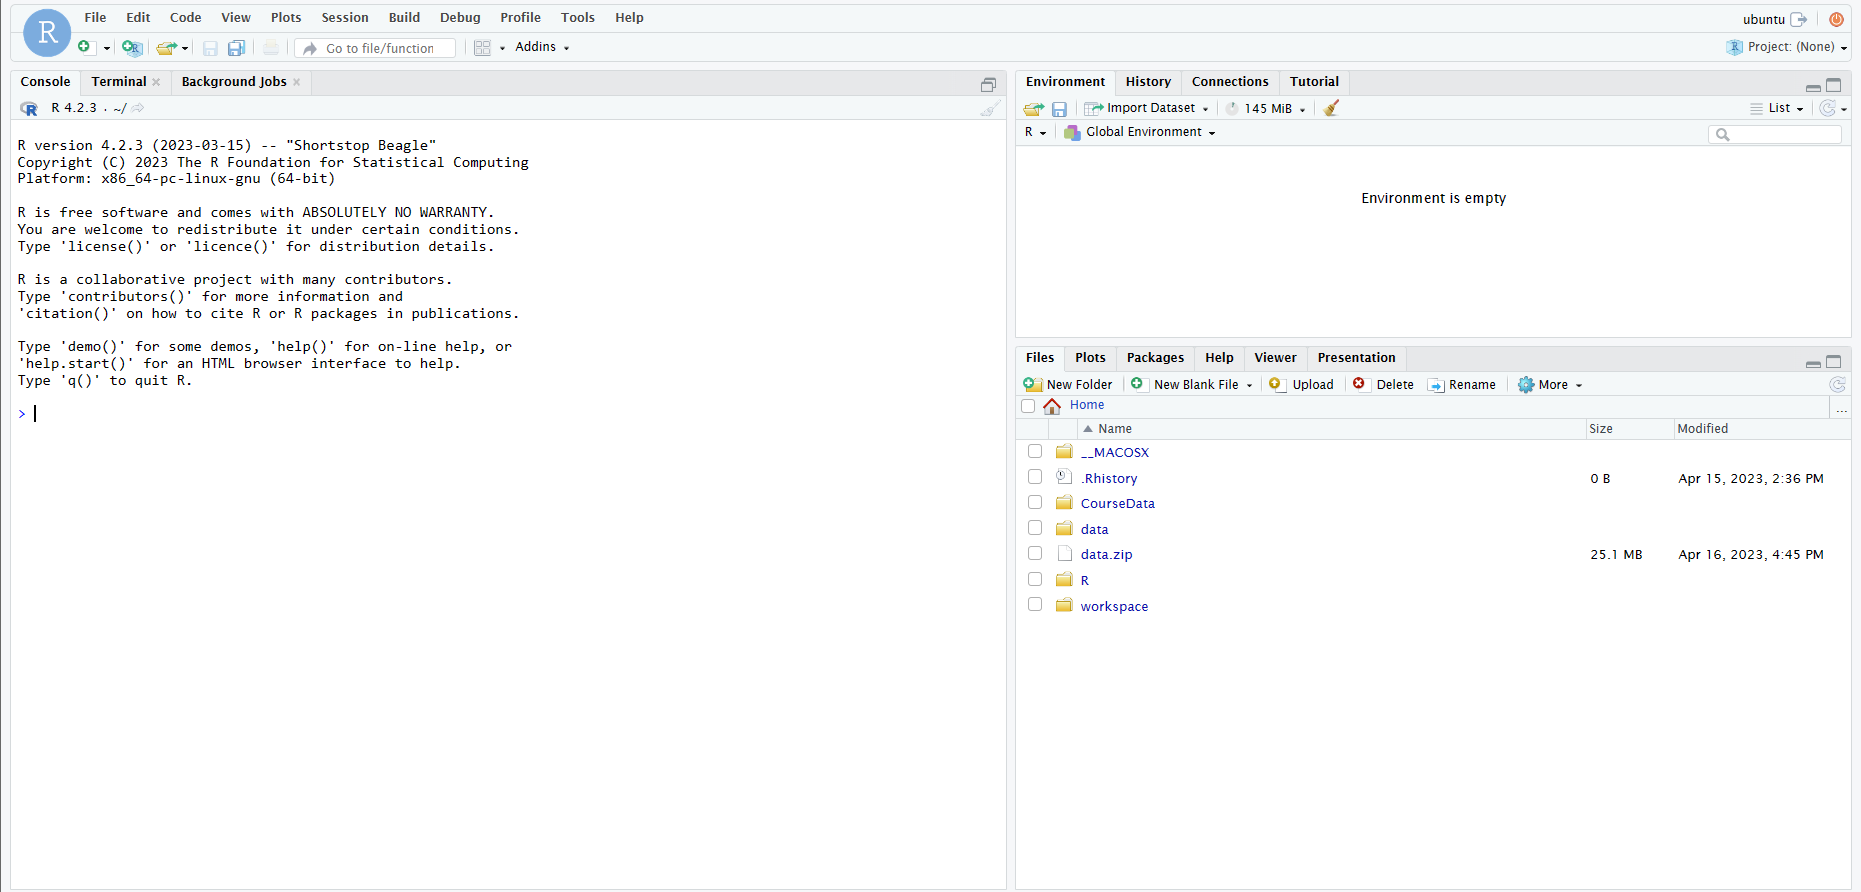
\includegraphics[keepaspectratio]{img/module_5_img_2.png}}

\begin{enumerate}
\def\labelenumi{\arabic{enumi}.}
\setcounter{enumi}{2}
\tightlist
\item
  Load up \texttt{Module\_5\_Lab.Rmd} by clicking {[}File{]} -\textgreater{} {[}Open File{]} -\textgreater{} {[}Select the .Rmd file in \texttt{module5} directory{]}
\end{enumerate}

If you have successfully opened the \texttt{.Rmd} file, you will see the following screen:

\pandocbounded{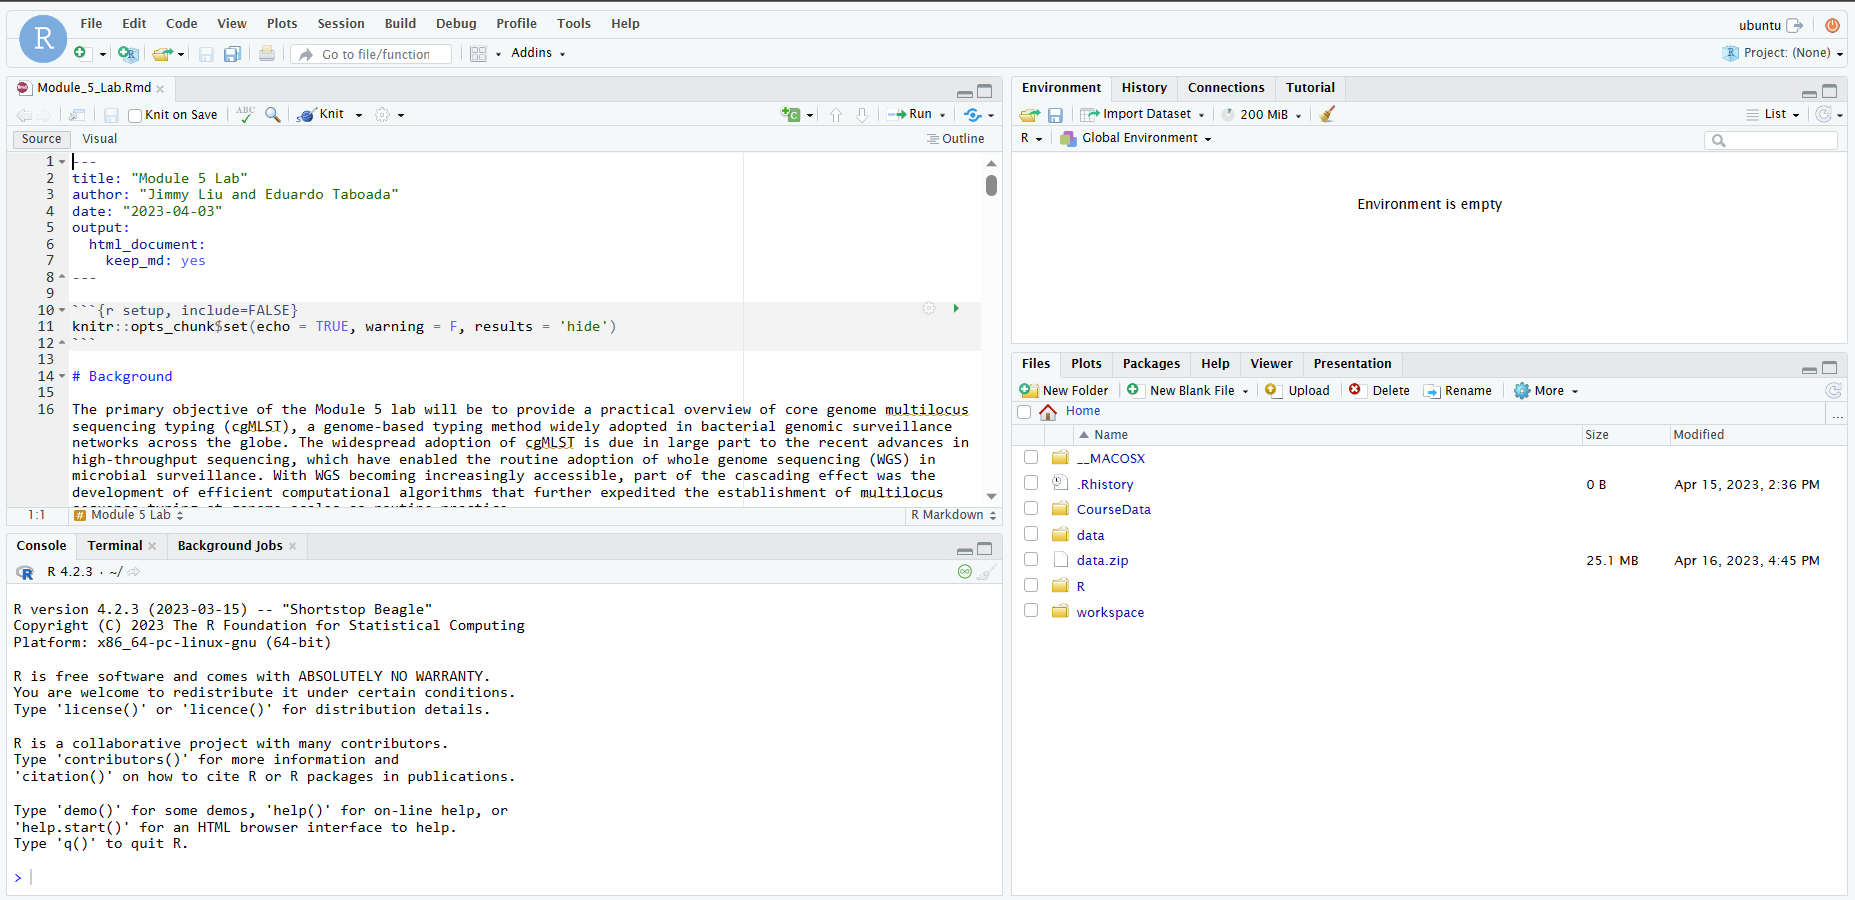
\includegraphics[keepaspectratio]{img/module_5_img_3.png}}

\subsection{Background}\label{background}

The primary objective of the Module 5 lab will be to provide a practical overview of core genome multilocus sequencing typing (cgMLST), a genome-based typing method widely adopted in bacterial genomic surveillance networks across the globe. The widespread adoption of cgMLST is due in large part to the recent advances in high-throughput sequencing, which have enabled the routine adoption of whole genome sequencing (WGS) in microbial surveillance. With WGS becoming increasingly accessible, part of the cascading effect was the development of efficient computational algorithms that further expedited the establishment of multilocus sequence typing at genome scales as routine practice.

The implementation of cgMLST by the PulseNet International network for foodborne outbreak surveillance has made it possible for WGS data to be used as evidence in public health investigations. Here, you will work with cgMLST data to conduct a retrospective analysis on a dataset that includes a number of possible Salmonella enterica outbreaks. Salmonella, which is primarily transmitted to humans through the consumption of contaminated foods, is one of the leading enteric pathogens in Canada and across the globe and was the first pathogen for which comprehensive genomic surveillance was implemented in Canada.

The outbreak dataset consists of WGS data from isolates recovered from samples collected from a diverse range of geographical regions, environments, and timelines that can be dated back to the early 2000s. Curating this outbreak dataset involved querying a global bacterial genomic surveillance database (GenomeTrakr) and PubMed queries to identify peer-reviewed publications that reported retrospective genomic analysis of Salmonella outbreaks. In this exercise, you will use a custom workflow written in the R language for statistical computing that includes modules to perform various steps in genomic epidemiologic analysis using cgMLST data. Your challenge will be to leverage the tools and data at your disposal to establish high quality cgMLST profiles that can be used to infer genetic relatedness and to explore patterns in the data in order to synthesize possible interpretations based on all available genomic and epidemiological data.

To start, you are provided with pre-computed cgMLST allele calls generated by chewBBACA (\href{https://pubmed.ncbi.nlm.nih.gov/29543149/}{Silva et al.~2018}, using a Salmonella core genome scheme based on 3,000 loci downloaded from \href{https://zenodo.org/record/4724927}{here}. Minor filtering has been performed to remove loci with zero informative alleles across the entire dataset. The following code template was used to call chewBBACA on a set of Salmonella genomes consolidated in a single directory called \texttt{/path/to/my\_genomes}:

\begin{verbatim}
chewBBACA.py AlleleCall -i /path/to/my_genomes/ -g /path/to/cgMLST_scheme/ -o /path/to/results
\end{verbatim}

\subsection{Learning Objectives}\label{learning-objectives}

\begin{itemize}
\tightlist
\item
  Understanding the significance of metrics used for MLST-based quality control
\item
  Explaining the difference between core, accessory and pan-genome loci and their use in MLST analysis
\item
  Building dendrograms from MLST data
\item
  Familiarisation with the ggtree R library for tree visualization
\item
  Exploring the clonality of bacterial populations in the context of bacterial foodborne outbreaks
\item
  Leveraging epidemiological data by linking it to MLST-based dendrograms to explain molecular differences and infer possible outbreak scenarios
\end{itemize}

\subsection{Analysis Dataset}\label{analysis-dataset}

The dataset for Module 5 lab has been uploaded to Google Sheets:

\begin{itemize}
\tightlist
\item
  \href{https://docs.google.com/spreadsheets/d/12gvH6U5pwj8QK-Ui3lOIYOm_X-69A2IE0cbctaEzY5E/edit?usp=sharing\#gid=1448009352}{Metadata}
\item
  \href{https://docs.google.com/spreadsheets/d/12gvH6U5pwj8QK-Ui3lOIYOm_X-69A2IE0cbctaEzY5E/edit?usp=sharing\#gid=8240612}{cgMLST data}
\end{itemize}

\subsection{Getting Started}\label{getting-started}

Let's begin by loading all R packages and helper scripts required to run all the code in this lab.

\emph{\ul{Every time you begin a new R session, you must reload all the packages and scripts!}}

\begin{verbatim}
suppressPackageStartupMessages(library(tidyverse))
suppressPackageStartupMessages(library(data.table))
suppressPackageStartupMessages(library(treedataverse))
suppressPackageStartupMessages(library(plotly))
suppressPackageStartupMessages(library(ggnewscale))
suppressPackageStartupMessages(library(ComplexHeatmap))
suppressPackageStartupMessages(library(circlize))
suppressPackageStartupMessages(library(randomcoloR))
suppressPackageStartupMessages(library(RColorBrewer))
suppressPackageStartupMessages(library(phangorn))
suppressPackageStartupMessages(library(knitr))
source("src/mlst_helper.R")
source("src/ggtree_helper.R")
source("src/cluster_helper.R")
\end{verbatim}

Next, read the cgMLST data and metadata into memory using \texttt{fread()} from the \texttt{data.table} package.

\begin{verbatim}
# data paths
metadata_path <- "data/senterica_metadata_final.tsv"
cgmlst_path <- "data/senterica_cgMLST_full.tsv"
# read file
meta <- fread(metadata_path, sep = "\t", colClasses = "character")
cgmlst <- fread(cgmlst_path, sep = "\t")
\end{verbatim}

\subsection{cgMLST QC}\label{cgmlst-qc}

Before proceeding any further, you will first evaluate cgMLST data quality. A number of quality criteria will be defined to determine whether the properties of the allele profiles meet quality standards. Incomplete genome assembly and reference bias during MLST scheme construction can introduce significant levels of missing information in MLST data in the form of unassigned alleles at various loci. Hence, care must be taken to avoid comparisons that include loci and genomes with excessive numbers of unassigned alleles that could reduce the precision of genetic similarity calculations to be used for generating dendrograms for inferring relationships between the various genomes in the dataset.

Below, you will conduct a series of steps to compute the frequency of unassigned alleles across each locus (i.e.~columns) and genome (i.e.~rows), which will inform the identification of poor quality loci/genomes that may need to be flagged for removal from downstream analyses.

\ul{Editable parts of the code have been highlighted in the code chunks.} You are highly encouraged to adjust them to observe how different parameters affect the outcome.

\subsection{Locus Quality}\label{locus-quality}

\begin{verbatim}
# use compute_lc helper function to compute 
# allele assignment rate (completeness) 
# across all loci
loci_completeness <- compute_lc(cgmlst)
# write to file
write.table(loci_completeness, "cgmlst_loci_quality.stats.tsv",
            quote = F, row.names = F, sep = "\t")
# print summary statistics for locus completeness
summary(loci_completeness)
\end{verbatim}

\begin{verbatim}
##     locus           valid_alleles   missing_alleles    completeness    
##  Length:2952        Min.   :  4.0   Min.   :  0.000   Min.   :  2.198  
##  Class :character   1st Qu.:181.0   1st Qu.:  0.000   1st Qu.: 99.451  
##  Mode  :character   Median :182.0   Median :  0.000   Median :100.000  
##                     Mean   :180.1   Mean   :  1.885   Mean   : 98.964  
##                     3rd Qu.:182.0   3rd Qu.:  1.000   3rd Qu.:100.000  
##                     Max.   :182.0   Max.   :178.000   Max.   :100.000
\end{verbatim}

\begin{verbatim}
##### EDITABLE VARIABLE #####
lqual_threshold <- 2
#############################

# identify low qual loci
lqual_loci <- loci_completeness %>% 
  filter(missing_alleles > lqual_threshold) %>% 
  pull(locus)
# remove low qual loci from input cgMLST data
cgmlst_lc <- cgmlst %>% select(-all_of(lqual_loci))
# write to file
write.table(cgmlst_lc, "cgmlst_lqual_loci_rm.tsv",
            quote = F, row.names = F, sep = "\t")
# print filtering results
message(paste("Number of loci before filter:", ncol(cgmlst)-1))
message(paste("Number of loci after filter:", ncol(cgmlst_lc)-1))
message(paste("Number of loci removed:", ncol(cgmlst)-ncol(cgmlst_lc)))
message(paste0("Loci with ", lqual_threshold, " or less missing alleles were retained"))
\end{verbatim}

\subsection{Defining Core Genes}\label{defining-core-genes}

\begin{verbatim}
##### EDITABLE VARIABLE #####
core_threshold <- 1
genome_qual <- 27
#############################

# compute core loci
core_loci <- calculate_core(
  mlst = cgmlst_lc,
  core_threshold = core_threshold,
  genome_qual = genome_qual
)
\end{verbatim}

\subsection{Genome Quality}\label{genome-quality}

\begin{verbatim}
# compute genome completeness
# given quality filtered scheme
genome_completeness <- cgmlst_lc %>% 
  select(1, all_of(core_loci)) %>% 
  compute_gc()
# write to file
write.table(genome_completeness, "cgmlst_genome_qual.stats.tsv",
            quote = F, row.names = F, sep = "\t")
# print data summary of genome completeness
summary(genome_completeness)
\end{verbatim}

\begin{verbatim}
##       ID            valid_alleles  missing_alleles   completeness   
##  Length:182         Min.   :2581   Min.   : 0.000   Min.   : 96.74  
##  Class :character   1st Qu.:2667   1st Qu.: 0.000   1st Qu.: 99.96  
##  Mode  :character   Median :2668   Median : 0.000   Median :100.00  
##                     Mean   :2664   Mean   : 4.275   Mean   : 99.84  
##                     3rd Qu.:2668   3rd Qu.: 1.000   3rd Qu.:100.00  
##                     Max.   :2668   Max.   :87.000   Max.   :100.00
\end{verbatim}

\begin{verbatim}
##### EDITABLE VARIABLE #####
lqual_g_threshold <- 26
#############################

# identify low qual genomes
lqual_genomes <- genome_completeness %>% 
  filter(missing_alleles > lqual_g_threshold) %>% 
  pull(ID)
# remove low qual genomes from quality filtered cgmlst
cgmlst_final <- cgmlst_lc %>% 
  filter(!(`#Name` %in% lqual_genomes)) %>% 
  select(1, all_of(core_loci))
# remove low qual genomes from metadata
metadata <- meta %>% filter(!(ID %in% lqual_genomes))
# write to file
write.table(cgmlst_final, "cgmlst_final.tsv",
            quote = F, row.names = F, sep = "\t")
# print filtering results
message(paste("Number of genomes before filter:", nrow(cgmlst_lc)))
message(paste("Number of genomes after filter:", nrow(cgmlst_final)))
message(paste("Number of genomes removed:", nrow(cgmlst_lc)-nrow(cgmlst_final)))
message(paste0("Genomes with ", lqual_g_threshold, " or less missing alleles were retained"))
\end{verbatim}

\subsection{Hamming Distance}\label{hamming-distance}

Distance-based and character-based methods can both be used to construct dendrograms from cgMLST data. However, the scope of this lab will only cover distance-based dendrograms, as character-based methods are covered extensively in other modules. In phylogenetic analysis, distance-based approaches are rather flexible in the sense that they can be constructed from any measure that quantifies genetic similarity, including distances computed by alignment-free (e.g.~Mash) or alignment-based (e.g.~BLAST) similarity search algorithms. Below, you are introduced to a metric called ``Hamming distance'', which is based on computing the number of differences between a pair of character vectors.

Given two character vectors of equal lengths, hamming distance is the total number of positions in which the two vectors are \ul{different:}

Profile A: \texttt{{[}\ 0\ ,\ 2\ ,\ 0\ ,\ 5\ ,\ 5\ ,\ 0\ ,\ 0\ ,\ 0\ ,\ 0\ {]}}

Profile B: \texttt{{[}\ 0\ ,\ 1\ ,\ 0\ ,\ 4\ ,\ 3\ ,\ 0\ ,\ 0\ ,\ 0\ ,\ 0\ {]}}

A != B: \texttt{{[}\ 0\ ,\ 1\ ,\ 0\ ,\ 1\ ,\ 1\ ,\ 0\ ,\ 0\ ,\ 0\ ,\ 0\ {]}}

Hamming distance = \texttt{sum(\ A\ !=\ B\ )} = 3

\begin{verbatim}
dist_mat <- cgmlst_final %>% 
  column_to_rownames("#Name") %>% 
  t() %>% 
  hamming()
# print matrix dimension
# the dimension should be symmetric!
dim(dist_mat)
\end{verbatim}

\begin{verbatim}
## [1] 172 172
\end{verbatim}

In the context of two cgMLST profiles, hamming distance can be calculated based on the number of allele differences across all loci. Hamming distances will be computed in an all vs all fashion to generate a pairwise distance matrix that will serve as the input for distance-based tree-building algorithms such as UPGMA and Neighbour-joining. We will visualize the clustering patterns in the distance matrix using the ComplexHeatmap package. We will also overlay serovar information to examine inter- and intra-serovar distances.

\begin{verbatim}
# create column annotations for heatmap
# to display serovar information
heatmap_annot <- metadata$serovar
names(heatmap_annot) <- metadata$ID
heatmap_annot <- heatmap_annot[order(factor(names(heatmap_annot),
                                            levels = rownames(dist_mat)))]
# create heatmap
dist_mat %>% 
  Heatmap(
    name = "cgMLST\nDistance",
    show_row_names = F, # do not display row labels
    show_column_names = F, # do not display column labels
    # use custom color gradient
    col = colorRamp2(
      c(min(dist_mat), mean(dist_mat), max(dist_mat)),
      c("#7ece97", "#eebd32", "#f76c6a")
    ),
    # add column annotation to show serovar info
    top_annotation = HeatmapAnnotation(
      Serovar = heatmap_annot,
      col = list(
                    "Serovar" = structure(brewer.pal(length(unique(heatmap_annot)), "Set1"),
                                                                names = unique(heatmap_annot))
      )
    )
  )
\end{verbatim}

\pandocbounded{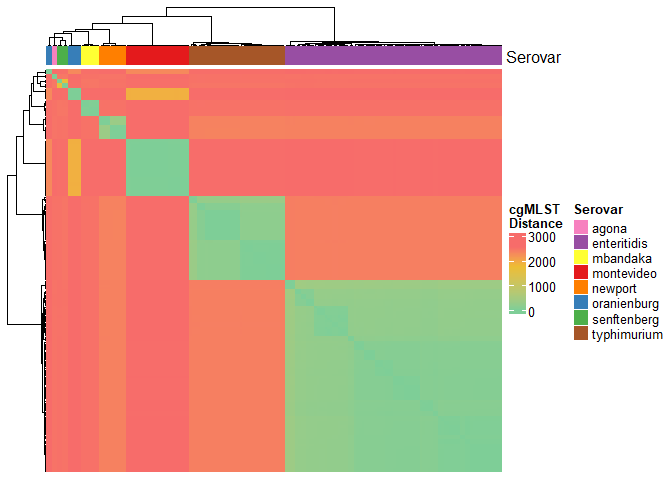
\includegraphics[keepaspectratio]{./img/distance-matrix.png}}

\subsection{Dendrogram Construction}\label{dendrogram-construction}

Here you will construct a neighbour-joining (NJ) tree using the \texttt{nj()} function from the ape package. Alternatively, a UPGMA tree can be constructed by simply replacing \texttt{method\ =\ \textquotesingle{}nj\textquotesingle{}} with \texttt{method\ =\ \textquotesingle{}upgma\textquotesingle{}} in the code chunk below.

To visualize the resulting dendrogram, you will interact with the R package \texttt{ggtree}, which offers an extensive suite of functions to manipulate, visualize, and annotate tree-like data structures. In this section, you will be introduced to the different visual capabilities of the \texttt{ggtree} package, and progressively update the same tree with several layers of visual annotations based on available metadata.

\subsection{A Simple Tree Vis}\label{a-simple-tree-vis}

To start, run the following code chunk to plot a circular tree of the entire dataset with the tree tips colored by serovar information.

You can assign a different metadata field to the \texttt{color\_var} variable to update the mapping of the color aesthetics in the tree. For example setting \texttt{color\_var\ =\ "Country"} will color the tree tips by the country of origin

\begin{verbatim}
##### EDITABLE VARIABLE #####
color_var <- "serovar"
#############################

# set random seed
set.seed(123)
# determine category count
# in the color aes variable
n_colors <- length(unique(pull(metadata, !!sym(color_var))))
# construct a core genome tree 
# using nj algorithm
cg_tree <- distance_tree(
  matrix = dist_mat,
  method = "nj"
)
# plot core genome tree and
# colouring the tree tips 
# by color_var
cg_tree_p <- cg_tree %>% 
  ggtree(layout = "circular",
         size = 0.75) %<+% metadata +
  geom_tippoint(aes(color = !!sym(color_var)),
                size = 2) +
  guides(color = guide_legend(override.aes = list(size = 3) ) ) +
  scale_color_manual(values = distinctColorPalette(n_colors))
# print tree plot object
cg_tree_p
\end{verbatim}

\pandocbounded{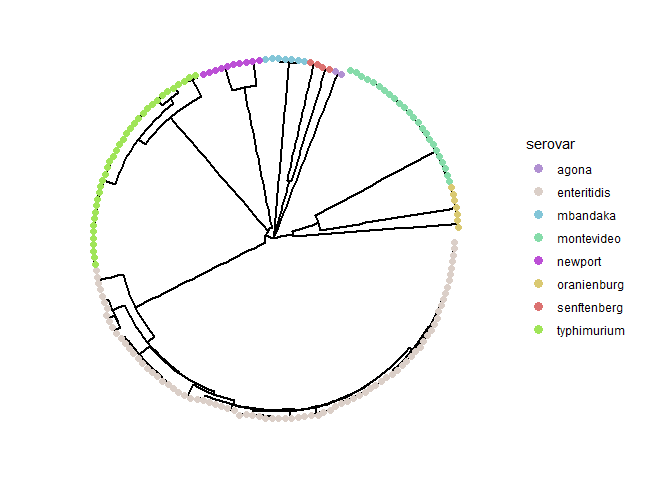
\includegraphics[keepaspectratio]{./img/core-genome-tree.png}}

\subsection{Clustering by Distance}\label{clustering-by-distance}

Identifying clusters of genomes sharing highly similar cgMLST profiles through the application of distance thresholds is a common practice in genomic surveillance and epidemiological investigations. Detecting novel clusters, comprising pathogen isolates from human clinical cases, can signal the emergence of an outbreak requiring a public health response and can provide important epidemiological insights on outbreak progression. Similarly, the co-clustering of outbreak isolates with isolates from food/environmental sources can help link the outbreak to possible sources/reservoirs of the pathogen in order to inform prevention and control measures.

In this section, you will generate genomic clusters from the dataset by applying several distance cutoffs. You will then place clusters within the dendrogram and analyze cluster memberships to spot possible outbreaks in the dataset.

\begin{verbatim}
# define clustering distance cutoffs
dist_cutoff <- c(0, seq(5, 100, 5), seq(200, 1000, 100))
# perform complete linkage clustering
hclust_res <- map(dist_cutoff, function(x) {
  dist_mat %>% 
    as.dist() %>% 
    hclust(method = "complete") %>% 
    cutree(h = x) %>% 
    as.factor()
})
names(hclust_res) <- paste0("clust_", dist_cutoff)
# print clustering results table
(
  clusters <- data.frame(hclust_res) %>% 
    rownames_to_column("ID")
  )
\end{verbatim}

Let's now superimpose the clustering information on the previous tree to examine whether the above code chunk has generated sensible cluster assignments. Run the code chunk below to insert text labels that span across tree tips assigned to the same clusters at \ul{a specified threshold}.

You can update the \texttt{target\_threshold} variable to examine how cluster membership changes in response to clustering distance cutoffs.

\begin{verbatim}
### EDITABLE VARIABLE ###
target_threshold <- 500
#########################

# variable to subset clusters
target_variable <- paste0("clust_", target_threshold)

# create cluster group list object
cluster_grp <- clusters %>% 
  select(ID, target_variable) %>%
  group_by(!!sym(target_variable)) %>% 
  {setNames(group_split(.), group_keys(.)[[1]])} %>% 
  map(~pull(., ID))
# sequester singleton clusters
cluster_grp <- cluster_grp[which(map_dbl(cluster_grp, ~length(.)) > 1)]

# create serovar group list object
serovar_grp <- metadata %>% 
  select(ID, serovar) %>% 
  split(f = as.factor(.$serovar)) %>% 
  map(~pull(., ID))

# add cluster memberships and serovar information
# to tree object
cg_tree <- groupOTU(cg_tree, cluster_grp, 'Clusters')
cg_tree <- groupOTU(cg_tree, serovar_grp, 'Serovars')

# plot core genome tree where
# colored blocks = clusters 
# text annotations = serovars
cg_tree %>% 
  ggtree(layout='circular', # tree shape
         size = 1 # branch width
  ) +
  # add colored blocks to display serovars
  geom_hilight(
    mapping = aes(
      node = node,
      fill = Serovars,
      subset = node %in% map_dbl(
        serovar_grp,
        ~getMRCA(cg_tree, .)
        )
      )
    ) +
  # add text annotations to display clusters
  geom_cladelab(
    mapping = aes(
      node = node,
      label = Clusters,
      subset = node %in% map_dbl(
        cluster_grp,
        ~getMRCA(cg_tree, .)
      )
    ),
    horizontal=T,
    angle = 'auto',
    barsize = 0.75,
    offset = 50,
    offset.text = 50,
    align = T
  ) +
  # legend parameters
  guides(fill = guide_legend(
    nrow = 9,
    override.aes = list(alpha = 0.8)
    )
  ) +
  labs(fill = "Serovar") +
  scale_fill_brewer(palette = "Paired")
\end{verbatim}

\pandocbounded{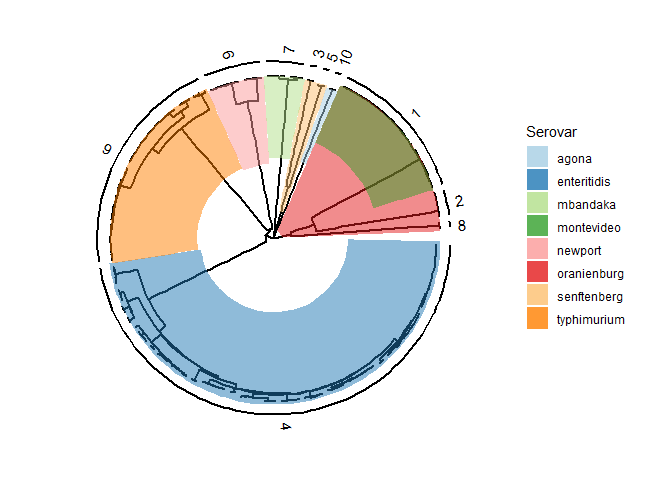
\includegraphics[keepaspectratio]{./img/cg-tree-cluster.png}}

\subsection{Cluster Analysis}\label{cluster-analysis}

In order to analyze the clustering patterns in the core genome tree at greater resolutions, you will work with a number of R functions introduced below. These functions are intended to be used in conjunction to zoom in on specific bacterial populations in the dataset that would empower you to explore the clonality and epidemiology of target strains.

\subsubsection{serovar\_subtree}\label{serovar_subtree}

The purpose of the function \texttt{serovar\_subtree} is to analyze subtrees of specific serovars. The target serovar to examine is defined by the \texttt{serovar\_name} variable. Specifying a NULL value to the variable will display the entire tree.

The serovar tree can be annotated with cluster information \ul{at a specific threshold} in the form of tip-spanning text labels. The cluster membership annotations are defined by the variable, \texttt{distance\_threshold}.

\begin{verbatim}
# NOTE: there needs to be a comma at the end of each line!
serovar_subtree(
  tree = cg_tree,
  serovar_name = NULL, # which serovar cluster to visualize?
  distance_threshold = 10, # the dist threshold used for cluster definition?
  color_by = "serovar", # which metadata variable to color tree tips by?
  color.tiplab = F, # whether to color tip labels
  tip.size = 4, # size of tree tip point
  label_vars = c("geo_loc", "iso_date", "iso_source"), # metadata vars only
  label.offset = 80, # distance between labels and tree tips
  label.size = 5, # tree tip label text size
  legend.x = 0.23, # legend position on x axis
  legend.y = 0.9, # legend position on y axis
  legend.size = 6, # legend text size
  legend.ncat.per.col = 8, # number of categories to show per column in legend
  hide.legend = F, # whether to hide colour legend
  plot.xlim = 2300, # plot area width
  annot.offset = 3, # distance between heatmap and tree tips
  annot.textsize = 5, # heatmap x axis text label size
  annot.barsize = 0.75, # annotation bar width
  show.title = T # whether to display distance threshold
)
\end{verbatim}

\begin{verbatim}
# export tree to pdf format
ggsave("serovar_subtree.pdf", height = 30, width = 16)
\end{verbatim}

\subsubsection{cluster\_subtree}\label{cluster_subtree}

The purpose of the function \texttt{cluster\_subtree} is to analyze subtrees of specific clusters defined at a given distance threshold. A cluster is defined by its ID and the distance threshold used for assignment, which are defined by the variables cluster\_name and distance\_threshold, respectively. Note that you will need to utilize the serovar\_subtree to identify the IDs of clusters of interest.

\begin{verbatim}
# NOTE: there needs to be a comma at the end of each line!
cluster_subtree(
  tree = cg_tree,
  clusters = clusters,
  distance_threshold = 25, # the dist threshold used for cluster definition?
  cluster_name = "1", # cluster ID to visualize?
  color_by = "country", # which metadata variable to color tree tips by?
  color.tiplab = F, # whether to color tip labels
  tip.size = 3, # size of tree tip point
  legend.x = 0.1, # legend position on x axis
  legend.y = 0.85, # legend position on y axis
  legend.size = 5, # legend text size
  legend.ncat.per.col = 8, # number of categories to show per column in legend
  hide.legend = F, # whether to hide colour legend
  plot.xlim = 30, # plot area width
  label_vars = c("country", "iso_date", "iso_source"), # metadata vars only
  label.offset = 5.5, # distance between labels and tree tips
  label.size = 4, # tree tip label text size
  annot.offset = 0.1, # distance between heatmap and tree tips
  annot.width = 0.4, # heatmap width
  annot.textsize = 4, # heatmap x axis text label size
  annot.nthreshold = 6 # number of clustering thresholds to display
)
\end{verbatim}

\pandocbounded{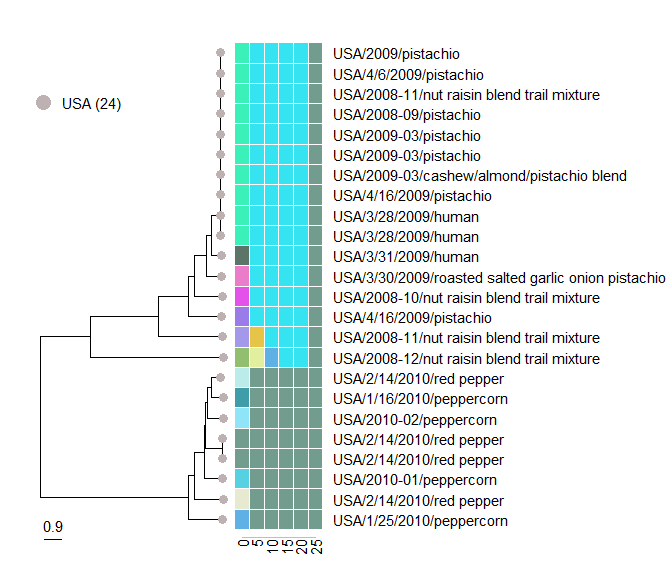
\includegraphics[keepaspectratio]{./img/cluster-subtree.png}}

\subsubsection{cluster\_summary}\label{cluster_summary}

The purpose of the function \texttt{cluster\_summary} is to compare the distribution of the categorical data in the metadata between clusters defined at a distance threshold. For example, these comparisons can provide a global summary of the putative sources of origin and geographical spread of each genomic cluster.

\begin{verbatim}
# NOTE: there needs to be a comma at the end of each line!
cluster_summary(
  distance_threshold = 10, # the dist threshold used for cluster definition?
  serovar_name = NULL, # which serovar to include?
  vars = c("geo_loc","iso_source", "iso_date_ym"), # metadata vars only
  panel.ncol = 1, # number of columns to arrange the panels in
  rm.low.freq.clust = T, # whether to remove low frequency (N < 4) clusters
  interactive = T # whether to generate interactive plots
)
\end{verbatim}

\subsection{Investigating Local Core Genes}\label{investigating-local-core-genes}

\begin{verbatim}
# identify a local core genome scheme
# for a target cluster and build tree
local_tree <- local_cg_tree(
  core_mlst = cgmlst_final,
  full_mlst = cgmlst_lc,
  distance_threshold = 100, # the dist threshold used for cluster definition?
  cluster_name = "10", # cluster ID to analyze?
  core_threshold = 1, # minimum number of missing alleles allowed
  method = "nj" # tree method: nj or upgma
)
# perform complete linkage clustering
hclust_res_local <- map(dist_cutoff, function(x) {
  cophenetic.phylo(local_tree) %>% 
    as.dist() %>% 
    hclust(method = "complete") %>% 
    cutree(h = x) %>% 
    as.factor()
})
names(hclust_res_local) <- paste0("clust_", dist_cutoff)
# create clusters data frame
clusters_local <- data.frame(hclust_res_local) %>% 
    rownames_to_column("ID")
\end{verbatim}

\begin{verbatim}
plot_subtree(
  tree = local_tree,
  clusters = clusters_local,
  color_by = "country", # which metadata variable to color tree tips by?
  color.tiplab = F, # whether to color tip labels
  tip.size = 3, # size of tree tip point
  legend.x = 0.15, # legend position on x axis
  legend.y = 0.85, # legend position on y axis
  legend.size = 5, # legend text size
  legend.ncat.per.col = 8, # number of categories to show per column in legend
  hide.legend = F, # whether to hide colour legend
  plot.xlim = 150, # plot area width
  label_vars = c("country", "iso_date", "iso_source"), # metadata vars only
  label.offset = 25, # distance between labels and tree tips
  label.size = 4, # tree tip label text size
  annot.offset = 0.1, # distance between heatmap and tree tips
  annot.width = 0.3, # heatmap width
  annot.textsize = 4, # heatmap x axis text label size
  annot.nthreshold = 6 # number of clustering thresholds to display
)
\end{verbatim}

\pandocbounded{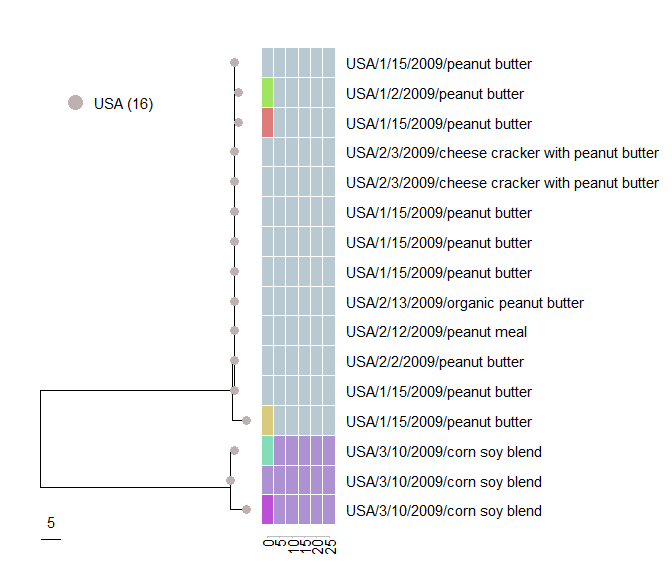
\includegraphics[keepaspectratio]{./img/plot-local-cg-tree.png}}

\subsection{Group Exercise}\label{group-exercise}

\begin{enumerate}
\def\labelenumi{\arabic{enumi}.}
\item
  Review the cgMLST profiles before and after the removal of low quality genomes, and identify two samples that exceed \textgreater1\% unassigned alleles (i.e.~with more than 26 unassigned alleles).
\item
  Review the circular tree and identify which serovar(s) is/are not monophyletic (i.e.~serovars that are distributed in multiple areas of the tree).
\item
  Use one of the following functions or in combination: serovar\_subtree(), cluster\_subtree(), cluster\_summary() to analyse one particular serovar and identify three clusters that likely correspond to different outbreaks.
\item
  Identify genomic clusters that fit the following criteria and consider possible scenarios for interpretation of genomic data and epidemiological metadata:
\end{enumerate}

\begin{enumerate}
\def\labelenumi{\alph{enumi}.}
\tightlist
\item
  A genomic cluster comprising human clinical cases with similar geographical and temporal information
\item
  A genomic cluster in which the human clinical cases are dispersed in geography and/or time
\item
  A genomic cluster in which human clinical isolates cluster with non-human isolates from a particular source type
\item
  A genomic cluster in which human clinical isolates cluster with non-human isolates from multiple source types.
\item
  Genomes from different genomic clusters identified within a single putative outbreak that can be linked to a common source
\end{enumerate}

\begin{enumerate}
\def\labelenumi{\arabic{enumi}.}
\setcounter{enumi}{4}
\item
  Is it important to analyze clusters at different distance cutoffs? Why?
\item
  What functional products could be encoded by the accessory loci in the data?
\end{enumerate}

Congratulations! You have completed Lab 5!

\chapter{Module 6: Antimicrobial Resistant Gene (AMR) Analysis}\label{module-6-antimicrobial-resistant-gene-amr-analysis}

\section{Lecture}\label{lecture-5}

\section{Lab}\label{lab-3}

\subsection{Introduction}\label{introduction-1}

This module gives an introduction to prediction of antimicrobial resistome and phenotype based on comparison of genomic or metagenomic DNA sequencing data to reference sequence information. While there is a large diversity of reference databases and software, this tutorial is focused on the Comprehensive Antibiotic Resistance Database (\href{http://card.mcmaster.ca/}{CARD}) for genomic AMR prediction.

There are several databases (see \href{https://www.nature.com/articles/s41576-019-0108-4/tables/2}{here} for a list) which try and organise information about AMR as well as helping with interpretation of resistome results. Many of these are either specialised on a specific type of resistance gene (e.g., \href{http://bldb.eu/}{beta-lactamases}), organism (e.g., \href{https://github.com/jodyphelan/tbdb}{\emph{Mycobacterium tuberculosis}}), or are an automated amalgamation of other databases (e.g., \href{https://megares.meglab.org/}{MEGARes}). There are also many tools for detecting AMR genes each with their own strengths and weaknesses (see this \href{https://www.frontiersin.org/articles/10.3389/fpubh.2019.00242/full}{paper} for a non-comprehensive list of tools!).

The ``Big 3'' databases that are comprehensive (involving many organisms, genes, and types of resistance), regularly updated, have their own gene identification tool(s), and are carefully maintained and curated are:

\begin{enumerate}
\def\labelenumi{\arabic{enumi}.}
\tightlist
\item
  Comprehensive Antibiotic Resistance Database (\href{http://card.mcmaster.ca/}{CARD}) with the Resistance Gene Identifier (\href{https://github.com/arpcard/rgi}{RGI})
\item
  National Center for Biotechnology Information's National Database of Antibiotic Resistant Organisms (\href{https://www.ncbi.nlm.nih.gov/pathogens/antimicrobial-resistance/}{NDARO}) with \href{https://www.ncbi.nlm.nih.gov/pathogens/antimicrobial-resistance/AMRFinder/}{AMRFinderPlus}
\item
  \href{https://cge.cbs.dtu.dk/services/ResFinder/}{ResFinder} database with its associated \href{https://cge.cbs.dtu.dk/services/ResFinder/}{ResFinder} tool
\end{enumerate}

In this practical we are going to focus on CARD and the associated RGI tool because:

The \href{https://card.mcmaster.ca/ontology/36006}{Antibiotic Resistance Ontology} it is built upon is a great way to organize information about AMR.
CARD is the most heavily used database internationally, with over 5000 citations.
We are biased. CARD is Canadian and pretty much all the CBW faculty collaborate or are part of the group that develops CARD! See \href{https://pubmed.ncbi.nlm.nih.gov/36263822/}{Alcock et al.~2023. CARD 2023: expanded curation, support for machine learning, and resistome prediction at the Comprehensive Antibiotic Resistance Database. Nucleic Acids Research, 51, D690-D699}.

\subsection{CARD Website and Antibiotic Resistance Ontology}\label{card-website-and-antibiotic-resistance-ontology}

The relationship between AMR genotype and AMR phenotype is complicated and no tools for complete prediction of phenotype from genotype exist. Instead, analyses focus on prediction or catalog of the AMR resistome - the collection of AMR genes and mutants in the sequenced sample. While BLAST and other sequence similarity tools can be used to catalog the resistance determinants in a sample via comparison to a reference sequence database, interpretation and phenotypic prediction are often the largest challenge. To start the tutorial, we will use the Comprehensive Antibiotic Resistance Database (\href{http://card.mcmaster.ca/}{CARD}) website to examine the diversity of resistance mechanisms, how they influence bioinformatics analysis approaches, and how CARD's \href{https://card.mcmaster.ca/ontology/36006}{Antibiotic Resistance Ontology} (ARO) can provide an organizing principle for interpretation of bioinformatics results.

CARD's website provides the ability to:

\begin{itemize}
\tightlist
\item
  Browse the \href{https://card.mcmaster.ca/ontology/36006}{Antibiotic Resistance Ontology} (ARO) and associated knowledgebase.
\item
  Browse the underlying AMR detection models, reference sequences, and SNP matrices.
\item
  Download the ARO, reference sequence data, and indices in a number of formats for custom analyses.
\item
  Perform integrated genome analysis using the Resistance Gene Identifier (RGI).
\end{itemize}

In this part of the tutorial, your instructor will walk you through the following use of the CARD website to familiarize yourself with its resources:

\begin{enumerate}
\def\labelenumi{\arabic{enumi}.}
\tightlist
\item
  What are the mechanisms of resistance described in the Antibiotic Resistance Ontology?
\item
  Examine the NDM-1 beta-lactamase protein, it's mechanism of action, conferred antibiotic resistance, it's prevalence, and it's detection model.
\item
  Examine the AAC(6')-Iaa aminoglycoside acetyltransferase, it's mechanism of action, conferred antibiotic resistance, it's prevalence, and it's detection model.
\item
  Examine the fluoroquinolone resistant gyrB for M. tuberculosis, it's mechanism of action, conferred antibiotic resistance, and it's detection model.
\item
  Examine the MexAB-OprM efflux complex with MexR mutations, it's mechanism of action, conferred antibiotic resistance, it's prevalence, and it's detection model(s).
\end{enumerate}

\begin{enumerate}
\def\labelenumi{\arabic{enumi}.}
\tightlist
\item
  \begin{itemize}
  \tightlist
  \item
    antibiotic target alteration + antibiotic target replacement + antibiotic target protection + antibiotic inactivation + antibiotic efflux + reduced permeability to antibiotic + resistance by absence + modification to cell morphology + resistance by host-dependent nutrient acquisition 2. NDM-1: antibiotic inactivation; beta-lactams (penam, cephamycin, carbapenem, cephalosporin); over 40 pathogens (lots of ESKAPE pathogens) - note strong association with plasmids; protein homolog model 3. AAC(6')-Iaa: antibiotic inactivation; aminogylcosides; \emph{Salmonella enterica}; protein homolog model 4. gyrB: antibiotic target alteration; fluoroquinolones; \emph{Mycobacterium}; protein variant model 5. MexAB-OprM with MexR mutations: antibiotic efflux; broad range of drug classes; looking at MexA sub-unit: \emph{Pseudomonas}; efflux meta-model
  \end{itemize}
\end{enumerate}

\subsection{RGI for Genome Analysis}\label{rgi-for-genome-analysis}

As illustrated by the exercise above, the diversity of antimicrobial resistance mechanisms requires a diversity of detection algorithms and a diversity of detection limits. CARD's Resistance Gene Identifier (RGI) currently integrates four CARD detection models: \href{https://github.com/arpcard/rgi\#analyzing-genomes-genome-assemblies-metagenomic-contigs-or-proteomes-a-k-a-rgi-main}{Protein Homolog Model, Protein Variant Model, rRNA Variant Model, and Protein Overexpression Model}. Unlike naïve analyses, CARD detection models use curated cut-offs, currently based on BLAST/DIAMOND bitscore cut-offs. Many other available tools are based on BLASTN or BLASTP without defined cut-offs and avoid resistance by mutation entirely.

In this part of the tutorial, your instructor will walk you through the following use of CARD's \href{https://card.mcmaster.ca/analyze/rgi}{Resistome Gene Identifier} with default settings ``Perfect and Strict hits only'', ``Exclude nudge'', and ``High quality/coverage'':

\begin{itemize}
\tightlist
\item
  Resistome prediction for the multidrug resistant Acinetobacter baumannii MDR-TJ, complete genome (NC\_017847).
\item
  Resistome prediction for the plasmid isolated from Escherichia coli strain MRSN388634 plasmid (KX276657).
\item
  Explain the difference in fluoroquinolone resistance MIC between two clinical strains of \emph{Pseudomonas aeruginosa} that appear clonal based on identical MLST (\texttt{Pseudomonas1.fasta}, \texttt{Pseudomonas2.fasta} - these files can be found in this GitHub repo). Hint, look at SNPs.
\end{itemize}

The first two examples list the predicted resistome of the analyzed genome and plasmid, while the third example illustrates that \texttt{Pseudomonas2.fasta} contains an extra T83I mutation in gyrA conferring resistance to fluoroquinolones, above that provided by background efflux.

\subsection{RGI at the Command Line}\label{rgi-at-the-command-line}

RGI is a command line tool as well, so we'll do a demo analysis of 112 clinical multi-drug resistant \emph{E. coli} from Hamilton area hospitals, sequenced on MiSeq and assembled using SPAdes (an older genome assembler). We'll additionally try RGI's heat map tool to compare genomes.

Login into your course account's working directory and make a module6 directory:

\begin{verbatim}
cd ~/workspace
mkdir module6
cd module6
\end{verbatim}

Take a peak at the list of E. coli samples:

\begin{verbatim}
ls /home/ubuntu/CourseData/IDE_data/module6/ecoli
\end{verbatim}

RGI has already been installed using Conda, list all the available software in Conda, activate RGI, and then review the RGI help screen:

\begin{verbatim}
conda env list
conda activate rgi
rgi -h
\end{verbatim}

First we need to acquire the latest AMR reference data from the CARD website:

\begin{verbatim}
rgi load -h
wget https://card.mcmaster.ca/latest/data
tar -xvf data ./card.json
less card.json
rgi load --card_json ./card.json --local
ls
\end{verbatim}

We don't have time to analyze all 112 samples, so let's analyze 1 as an example (the course GitHub repo contains an EXCEL version of the resulting \texttt{C0001.txt} file). When analyzing FASTA files we use the \textbf{main} sub-command, here with default settings ``Perfect and Strict hits only'', ``Exclude nudge'', and ``High quality/coverage'':

\begin{verbatim}
rgi main -h
rgi main -i /home/ubuntu/CourseData/IDE_data/module6/ecoli/C0001_E_coli.contigs.fasta -o C0001 -t contig -a DIAMOND -n 4 --local --clean
ls
less C0001.json
less C0001.txt
column -t -s $'\t' C0001.txt  | less -S
\end{verbatim}

Default RGI \textbf{main} analysis of C0001 lists 17 Perfect annotations and 52 Strict annotations. Yet, 44 annotations are efflux components common in \emph{E. coli} that may or may not lead to clinical levels of AMR. Nonetheless, outside of efflux there are some antibiotic inactivation, target replacement, or target alteration genes known to be high risk (e.g., sul1, TEM-1, CTX-M-15, APH(6)-Id, and gyrA mutations). This is a MDR isolate of \emph{E. coli}.

What if these results did not explain our observed phenotype? We might want to explore the RGI Loose hits (the course GitHub repo contains an EXCEL version of the resulting \href{https://github.com/bioinformaticsdotca/IDE_2023/blob/main/module6/rgi_main_results/C0001_IncludeLoose.xlsx}{C0001\_IncludeLoose.txt} file), shown here with settings ``Perfect, Strict, and Loose hits'', ``Include nudge'', and ``High quality/coverage'':

\begin{verbatim}
rgi main -h
rgi main -i /home/ubuntu/CourseData/IDE_data/module6/ecoli/C0001_E_coli.contigs.fasta -o C0001_IncludeLoose -t contig -a DIAMOND -n 4 --local --clean --include_nudge --include_loose
ls
column -t -s $'\t' C0001_IncludeLoose.txt  | less -S
\end{verbatim}

An additional 3 nudged Strict annotations (\emph{Escherichia coli} PtsI with mutation conferring resistance to fosfomycin, EC-5 beta-lactamase, \emph{Escherichia coli} EF-Tu mutants conferring resistance to pulvomycin) and 390 Loose annotations have been added to investigate for leads that could explain the observed phenotype. Note this scenario is unlikely for clinical isolates given CARD's reference data, but is possible for environmental isolates.

We have pre-compiled results for all 112 samples under ``Perfect and Strict hits only'', ``Exclude nudge'', and ``High quality/coverage'', so let's try RGI's heat map tool (\href{https://github.com/bioinformaticsdotca/IDE_2023/tree/main/module6/rgi_main_results}{pre-compiled images} can be downloaded from the course GitHub repo) (please ignore the FutureWarning):

\begin{verbatim}
ls /home/ubuntu/CourseData/IDE_data/module6/ecoli_json
rgi heatmap -h
rgi heatmap -i /home/ubuntu/CourseData/IDE_data/module6/ecoli_json -o genefamily_samples --category gene_family --cluster samples
rgi heatmap -i /home/ubuntu/CourseData/IDE_data/module6/ecoli_json -o drugclass_samples --category drug_class --cluster samples
rgi heatmap -i /home/ubuntu/CourseData/IDE_data/module6/ecoli_json -o cluster_both --cluster both
rgi heatmap -i /home/ubuntu/CourseData/IDE_data/module6/ecoli_json -o cluster_both_frequency --frequency --cluster both
ls
\end{verbatim}

The last analysis is the most informative, showing that many of these isolates share the same complement of efflux variants, yet most isolates are unique in their resistome, with a subset sharing TEM-1, sul1, and other higher risk genes.

\subsection{RGI for Merged Metagenomic Reads}\label{rgi-for-merged-metagenomic-reads}

The standard RGI tool can be used to analyze metagenomics read data, but only for assembled or merged reads with Prodigal calling of partial open reading frames (ORFs). Here we will demonstrate analysis of merged reads. This is a computationally expensive approach, since each merged read set may contain a partial ORF, requiring RGI to perform massive amounts of BLAST/DIAMOND analyses. While computationally intensive (and thus generally not recommended), this does allow analysis of metagenomic sequences in protein space, including key substitutions, overcoming issues of high-stringency read mapping relative to nucleotide reference databases.

Lanza et al.~(\href{https://www.ncbi.nlm.nih.gov/pubmed/29335005}{Microbiome 2018, 15:11}) used AMR gene bait capture to sample human gut microbiomes for AMR genes. Using the \href{https://card.mcmaster.ca/analyze/rgi}{online RGI} under ``Perfect, Strict and Loose hits'', ``Include nudge'', and ``Low quality/coverage'' settings, analyze the first 500 merged metagenomic reads from their analysis (file \texttt{ResCap\_first\_500.fasta}). Take a close look at the predicted ``sul2'' and ``sul4'' hits in the results table. How good is the evidence for these AMR genes in this enriched metagenomics sample?

There are three merged reads with 100\% identity to \textasciitilde25\% of the sul2 gene each, while the 9 merged reads annotated as the sul4 gene encode less than 50\% identity to the reference sul2 protein, suggesting they are spurious annotations.

\subsection{Metagenomic Sequencing Reads and the KMA Algorithm}\label{metagenomic-sequencing-reads-and-the-kma-algorithm}

The most common tools for metagenomic data annotation are based on high-stringency read mapping, such as the \href{https://bitbucket.org/genomicepidemiology/kma/src/master}{KMA read aligner} due to its {[}documented better performance for redundant databases such as CARD{]}(\url{https://github.com/arpcard/rgi\#analyzing-metagenomic-reads-a-k-a-rgi-bwt}. Available methods almost exclusively focus on acquired resistance genes (e.g., sequences referenced in CARD's protein homolog models), not those involving resistance via mutation. However, CARD and other AMR reference databases utilize reference sequences from the published literature with clear experimental evidence of elevated minimum inhibitory concentration (MIC). This has implications for molecular surveillance as sequences in agricultural or environmental samples may differ in sequence from characterized \& curated reference sequences, which are predominantly from clinical isolates, creating false negative results for metagenomic reads for these environments. As such, CARD's tools for read mapping can use either canonical CARD (reference sequences from the literature) or predicted AMR resistance alleles and sequence variants from bulk resistome analyses, i.e.~\href{https://card.mcmaster.ca/resistomes}{CARD Resistomes \& Variants data set}.

To demonstrate read mapping using RGI \textbf{bwt}, we will analyze a \textasciitilde160k paired read subset of the raw sequencing reads from Lanza et al.'s (\href{https://www.ncbi.nlm.nih.gov/pubmed/29335005}{Microbiome 2018, 15:11}) use of AMR gene bait capture to sample human gut microbiomes.

First we need to acquire the additional AMR reference data from the previous CARD website download:

\begin{verbatim}
rgi card_annotation -i ./card.json > card_annotation.log 2>&1
rgi load --card_json ./card.json --card_annotation card_database_v3.2.6.fasta --local
ls
\end{verbatim}

Let's take a look at the raw gut metagenomics data to remind ourselves of the FASTQ format:

\begin{verbatim}
ls /home/ubuntu/CourseData/IDE_data/module6/gut_sample
less /home/ubuntu/CourseData/IDE_data/module6/gut_sample/gut_R1.fastq
\end{verbatim}

We can now map the metagenomic reads to the sequences in CARD's protein homolog models using the KMA algorithm:

\begin{verbatim}
rgi bwt -1 /home/ubuntu/CourseData/IDE_data/module6/gut_sample/gut_R1.fastq -2 /home/ubuntu/CourseData/IDE_data/module6/gut_sample/gut_R2.fastq -a kma -n 4 -o gut_sample.kma --local
ls
\end{verbatim}

RGI \textbf{bwt} produces a LOT of output files, see the details at the \href{https://github.com/arpcard/rgi\#rgi-bwt-tab-delimited-output-details}{RGI GitHub repo}. First, let's look at the summary statistics:

\begin{verbatim}
cat gut_sample.kma.overall_mapping_stats.txt
ls
\end{verbatim}

However, the file we are most interested in for now is gut\_sample.kma.gene\_mapping\_data.txt and the course GitHub repo contains an EXCEL version for easy viewing, but let's look at it on the command line:

\begin{verbatim}
column -t -s $'\t' gut_sample.kma.gene_mapping_data.txt  | less -S
cut -f 1 gut_sample.kma.gene_mapping_data.txt | sort -u | wc -l
ls
\end{verbatim}

\begin{itemize}
\tightlist
\item
  Ignoring efflux, which AMR gene had the most mapped reads?
\item
  Ignoring efflux, which AMR gene had the highest \% coverage?
\item
  How many AMR genes were found in total?
\item
  From these results and what you know about assembly, what do you think are the advantages/disadvantages of read-based methods?
\end{itemize}

Top 5 (non-efflux) for number of mapped reads: * tet(Q) with 40345 reads * tet(X) with 7205 reads * ErmF with 6510 reads * CblA-1 with 4160 reads * tet(O) with 1608 reads Top 5 (non-efflux) for \% length coverage (all had 100\%): * tet(Q) * tet(X) * ErmF * CblA-1 * tet(O) 90 AMR genes had sequencing reads mapped. Read-based analyses advantages and disadvantages: * Higher sensitivity (we find as many AMR genes as possible) * Lower specificity (we are more likely to make mistakes when identifying AMR genes) * Incomplete data (we are likely to find fragments of genes instead of whole genes, this can lead to confusion between similar genes) * No genomic context (we don't know where a gene we detect comes from in the genome, is it associated with a plasmid?)

We can repeat the read mapping analysis, but include more sequence variants in the reference set by including the \href{https://card.mcmaster.ca/resistomes}{CARD Resistomes \& Variants data set}. First we need to acquire the Resistomes \& Variant data from the CARD website:

THE FOLLOWING STEPS TAKE TOO LONG, DO NOT PERFORM DURING DEMO SESSION, INSTEAD PLEASE VIEW PRE-COMPILED RESULTS. FEEL FREE TO TRY THESE STEPS OUTSIDE OF CLASS.

\begin{verbatim}
wget -O wildcard_data.tar.bz2 https://card.mcmaster.ca/latest/variants
mkdir -p wildcard
tar -xjf wildcard_data.tar.bz2 -C wildcard
gunzip wildcard/*.gz
rgi wildcard_annotation -i wildcard --card_json ./card.json -v 4.0.0 > wildcard_annotation.log 2>&1
rgi load --card_json ./card.json --wildcard_annotation wildcard_database_v4.0.0.fasta --wildcard_index ./wildcard/index-for-model-sequences.txt --card_annotation card_database_v3.2.6.fasta --local
\end{verbatim}

Map reads to canonical CARD (reference sequences from the literature) \textbf{plus} predicted AMR resistance alleles and sequence variants from bulk resistome analyses, i.e.~\href{https://card.mcmaster.ca/resistomes}{CARD Resistomes \& Variants data set}:

THE FOLLOWING STEPS TAKE TOO LONG, DO NOT PERFORM DURING DEMO SESSION, INSTEAD PLEASE VIEW PRE-COMPILED RESULTS. FEEL FREE TO TRY THESE STEPS OUTSIDE OF CLASS.

\begin{verbatim}
rgi bwt -1 /home/ubuntu/CourseData/IDE_data/module6/gut_sample/gut_R1.fastq -2 /home/ubuntu/CourseData/IDE_data/module6/gut_sample/gut_R2.fastq -a kma -n 4 -o gut_sample_wildcard.kma --local --include_wildcard
ls
\end{verbatim}

The pre-compiled results can be viewed in the EXCEL version of \texttt{gut\_sample\_wildcard.kma.gene\_mapping\_data.txt} in the GitLab repo, but let's first compare statistics, where you'll see we aligned some additional reads:

YOU CAN EXECUTE THESE COMMANDS AS WE HAVE PROVIDED PRE-COMPUTED RESULTS.

\begin{verbatim}
clear
cat /home/ubuntu/CourseData/IDE_data/module6/kmaresults/gut_sample.kma.overall_mapping_stats.txt
cat /home/ubuntu/CourseData/IDE_data/module6/kmaresults/gut_sample_wildcard.kma.overall_mapping_stats.txt
cut -f 1 /home/ubuntu/CourseData/IDE_data/module6/kmaresults/gut_sample_wildcard.kma.gene_mapping_data.txt | sort -u | wc -l
ls
\end{verbatim}

Looking at the pre-compiled EXCEL spreadsheet, note that we have more information based on \href{https://card.mcmaster.ca/resistomes}{CARD Resistomes \& Variants data set}, such as mappings to multiple alleles, flags for association with plasmids, and taxonomic distribution of the mapped alleles.

\begin{itemize}
\tightlist
\item
  Ignoring efflux, which AMR gene had the most mapped reads?
\item
  How many AMR genes were found in total?
\item
  Which genes associated with plasmids have the most mapped reads?
\end{itemize}

Top 5 (non-efflux) for number of mapped reads gives the same list but with more data: * tet(Q) with 42684 mapped reads (up from 40345 reads) * tet(X) with 7393 mapped reads (up from 7205 reads) * ErmF with 6987 mapped reads (up from 6510 reads) * CblA-1 with 4160 mapped reads (no change) * tet(O) with 1870 mapped reads (up from 1608 reads) 114 AMR genes had sequencing reads mapped (up from 90). Top 5 (plasmid associated) for number of mapped reads: * tet(X) with 7393 reads * acrD with 1881 Reads * APH(6)-Id with 1418 reads * sul2 with 961 reads * aad(6) with 99 reads

\subsection{Pathogen of Origin Prediction}\label{pathogen-of-origin-prediction}

If there is time in the tutorial, we will demonstrate how to predict pathogen-of-origin for the AMR gene reads in the gut metagenomics data using k-mers. Please note this algorithm is not yet published and is currently undergoing validation. It is also slow and has a high memory burden as algorithm optimization has yet to be performed.

First, the reference data needs to be formatted for k-mer analysis (see the details at the \href{https://github.com/arpcard/rgi\#using-rgi-kmer-query-k-mer-taxonomic-classification}{RGI GitHub repo}):

DO NOT ATTEMPT THESE COMMANDS ON THE CLASS SERVERS, THEY REQUIRE MORE MEMORY

\begin{verbatim}
rgi clean --local       
wget https://card.mcmaster.ca/latest/data
tar -xvf data ./card.json
rgi load --card_json ./card.json --local
rgi card_annotation -i ./card.json > card_annotation.log 2>&1       
rgi load -i ./card.json --card_annotation card_database_v3.2.6.fasta --local
wget -O wildcard_data.tar.bz2 https://card.mcmaster.ca/latest/variants
mkdir -p wildcard
tar -xjf wildcard_data.tar.bz2 -C wildcard
gunzip wildcard/*.gz
rgi load --card_json ./card.json --kmer_database ./wildcard/61_kmer_db.json --amr_kmers ./wildcard/all_amr_61mers.txt --kmer_size 61 --local --debug > kmer_load.61.log 2>&1
\end{verbatim}

Now we can predict pathogen-of-origin for our metagenomics analysis that included canonical CARD (reference sequences from the literature) \textbf{plus} predicted AMR resistance alleles and sequence variants from bulk resistome analyses, i.e.~\href{https://card.mcmaster.ca/resistomes}{CARD Resistomes \& Variants data set}:

DO NOT ATTEMPT THESE COMMANDS ON THE CLASS SERVERS, THEY REQUIRE MORE MEMORY

\begin{verbatim}
rgi kmer_query --bwt --kmer_size 61 --threads 4 --minimum 10 --input ./gut_sample_wildcard.kma.sorted.length_100.bam --output gut_sample_wildcard.pathogen --local
\end{verbatim}

The pre-compiled results can be viewed in the EXCEL version of \texttt{gut\_sample\_wildcard.pathogen\_61mer\_analysis.gene.txt} in the GitLab repo, but let's look at some extracted results for the genes outlined above:

\begin{longtable}[]{@{}
  >{\raggedright\arraybackslash}p{(\linewidth - 4\tabcolsep) * \real{0.0422}}
  >{\raggedright\arraybackslash}p{(\linewidth - 4\tabcolsep) * \real{0.1084}}
  >{\raggedright\arraybackslash}p{(\linewidth - 4\tabcolsep) * \real{0.8494}}@{}}
\toprule\noalign{}
\begin{minipage}[b]{\linewidth}\raggedright
\textbf{ARO term}
\end{minipage} & \begin{minipage}[b]{\linewidth}\raggedright
\textbf{Mapped reads with kmer DB hits}
\end{minipage} & \begin{minipage}[b]{\linewidth}\raggedright
\textbf{CARDkmer Prediction}
\end{minipage} \\
\midrule\noalign{}
\endhead
\bottomrule\noalign{}
\endlastfoot
tet(X) & 6951 & Escherichia coli (chromosome or plasmid): 1; Elizabethkingia anophelis (chromosome or plasmid): 1; \\
acrD & 1860 & Escherichia coli (chromosome): 102; Escherichia coli (chromosome or plasmid): 664; \\
APH(6)-Id & 1388 & Escherichia coli (chromosome or plasmid): 12; Salmonella enterica (chromosome or plasmid): 2; Vibrio parahaemolyticus (chromosome or plasmid): 1; Enterobacter hormaechei (chromosome or plasmid): 1; Acinetobacter baumannii (chromosome or plasmid): 1; Escherichia coli (plasmid): 3; \\
sul2 & 898 & Escherichia coli (chromosome or plasmid): 3; Bacillus anthracis (chromosome or plasmid): 2; Klebsiella pneumoniae (chromosome or plasmid): 1; Pseudomonas aeruginosa (chromosome or plasmid): 1; Salmonella enterica (chromosome or plasmid): 1; \\
EC-8 & 517 & Escherichia coli (chromosome): 127; Shigella boydii (chromosome): 1; Escherichia coli (chromosome or plasmid): 26; \\
APH(3'\,')-Ib & 387 & Escherichia coli (chromosome or plasmid): 3; Enterobacter hormaechei (chromosome or plasmid): 1; \\
aad(6) & 97 & none \\
CblA-1 & 0 & none \\
\end{longtable}

The AMR genes associated with plasmids according to the CARD Resistomes \& Variants data set cannot easily be assigned to a specific pathogen, while those like acrD and EC-8 that are predominantly known from chromosomes have a reliable pathogen-of-origin prediction.

Congratulations! You have completed Lab 6!

\chapter{Module 7: Phylodynamics and Transmission Dynamics}\label{module-7-phylodynamics-and-transmission-dynamics}

\section{Lecture}\label{lecture-6}

\section{Lab}\label{lab-4}

\subsection{1. Introduction}\label{introduction-2}

In this tutorial we will be using phylogenetics and metadata to try and better understand the underlying evolutionary, ecological, and epidemiological processes of the SARS-CoV-2 pathogen. This is a field of study and methodology known as phylodynamics.

We will be focusing on 3 types of analysis using a dataset derived from the following study which found evidence of SARS-CoV-2 spilling over from human infections into wildlife, evolving within wildlife, and then infecting a human:

Pickering\emph{, B., Lung}, O., Maguire*, F., et al.~Divergent SARS-CoV-2 variant emerges in white-tailed deer with deer-to-human transmission Nat Microbiol 7, 2011-2024 (2022). \url{https://doi.org/10.1038/s41564-022-01268-9}

These analyses are:

\begin{itemize}
\tightlist
\item
  Inferring a molecular clock model to estimate when deer were infected with a specific SARS-CoV-2 lineage
\item
  Ancestral state reconstruction to identify where this took place
\item
  Inference of episodic selection related to this zoonoses
\end{itemize}

Now the big caveat here is that a lot of these analyses (including some of the more classic epidemiological parameter estimation phylodynamics) are typically done using a Bayesian framework such as \href{http://www.beast2.org/}{BEAST}. However, these can be quite challenging to run from a logistics perspective in the context of a practical. To this end, we are instead going to focus on the more ``quick and dirty'' maximum likelihood approaches using tools designed more for the scale of SARS-CoV-2 genomics data.

If you are interested in phylodynamics more deeply, I recommend checking out some of the semi-regularly held ``\href{https://taming-the-beast.org/workshops/Taming-the-BEAST-Online/}{Taming the BEAST}'' workshops and the tutorials shared by the \href{http://www.beast2.org/tutorials/}{BEAST Developers}. Paul Lewis' \href{http://phyloseminar.org/recorded.html}{phyloseminar.org} lectures on Bayesian phylogenetics (\href{https://www.youtube.com/watch?v=4PWlnNsfz90}{part 1} and \href{https://www.youtube.com/watch?v=TLtOS--YwkU}{part 2}) are also an excellent place to start to learn the basic theory of Bayesian methods.

\subsection{2. List of Software for Tutorial}\label{list-of-software-for-tutorial}

\begin{itemize}
\tightlist
\item
  \href{https://docs.nextstrain.org/projects/augur/en/stable/index.html}{Augur}
\item
  \href{https://mafft.cbrc.jp/alignment/software/}{mafft}
\item
  \href{http://www.iqtree.org/}{iqtree}
\item
  \href{https://treetime.readthedocs.io/en/latest/}{treetime}
\item
  \href{https://auspice.us/}{Auspice}
\item
  \href{http://hyphy.org/}{HyPhy}
\item
  \href{http://hyphy.org/methods/selection-methods/}{aBSREL}
\end{itemize}

\subsection{3. Exercise Setup}\label{exercise-setup}

\subsubsection{3.1. Copy Data Files}\label{copy-data-files}

To begin, we will copy over the necesssary files to \texttt{\textasciitilde{}/workspace}.

\textbf{Commands}

\begin{verbatim}
cp -r ~/CourseData/IDE_data/module8/ ~/workspace
cd ~/workspace/module8
\end{verbatim}

When you are finished with these steps you should be inside the directory \texttt{/home/ubuntu/workspace/module8}. You can verify this by running the command \texttt{pwd.}

\textbf{Output after running} \texttt{pwd}

\begin{verbatim}
/home/ubuntu/workspace/module8
\end{verbatim}

You should also see a directory \texttt{data}/ in the current directory which contains all the input data. You can verify this by running \texttt{ls\ data}:

\textbf{Output after running} \texttt{ls\ data}

\begin{verbatim}
sequences.fasta     metadata.tsv     reference_MN908947.3.fasta     S.xml
\end{verbatim}

\subsubsection{3.2. Activate Environment}\label{activate-environment}

Next we will activate the \href{https://docs.conda.io/en/latest/}{conda} environment, which will have all the tools needed by this tutorial pre-installed. To do this please run the following:

\textbf{Commands}

\begin{verbatim}
conda activate signalcovtools
\end{verbatim}

You should see the command-prompt (where you type commands) switch to include (\texttt{signalcovtools}) at the beginning, showing you are inside this environment. You should also be able to run the \texttt{augur} command like \texttt{augur\ -\/-version} and see output:

\textbf{Output after running} \texttt{augur\ -\/-version}

\begin{verbatim}
augur 24.3.0
\end{verbatim}

\subsubsection{3.3. Find your IP Address}\label{find-your-ip-address}

Similar to yesterday, we will want to either use the assigned hostname (e.g., xx.uhn-hpc.ca where xx is your instance number) or find the IP address of your machine on AWS so we can access some files from your machine on the web browser. To find your IP address you can run:

\textbf{Commands}

\begin{verbatim}
curl http://checkip.amazonaws.com
\end{verbatim}

This should print a number like XX.XX.XX.XX. Once you have your address, try going to \url{http://xx.uhn-hpc.ca} or \url{http://IP-ADDRESS} and clicking the link for \textbf{module8}. This page will be referred to later to view some of our output files. In addition, the link \textbf{precomputed-analysis} will contain all the files we will generate during this lab (phylogenetic trees, etc).

\subsection{4. Phylodynamics Analysis}\label{phylodynamics-analysis}

The overall goal of this lab is to make use of a set of SARS-CoV-2 genomes sequenced and analyzed in the above study and then use associated metadata and phylodynamic methods to gain insight into where and when the zoonoses most likely occurred (and their evolutionary impact). To do this, we will mostly make use of the \href{https://docs.nextstrain.org/projects/augur/en/stable/index.html}{Augur} tool suite, which powers the \href{https://nextstrain.org/}{NextStrain} website. Within augur, the key tool actually being used for most of our inferences is \href{https://treetime.readthedocs.io/en/latest/}{TreeTime} a likelihood based tool for inferring molecular clocks and ancestral traits.

An overview of the basic usage of Augur (figure from the Augur documentation):

\pandocbounded{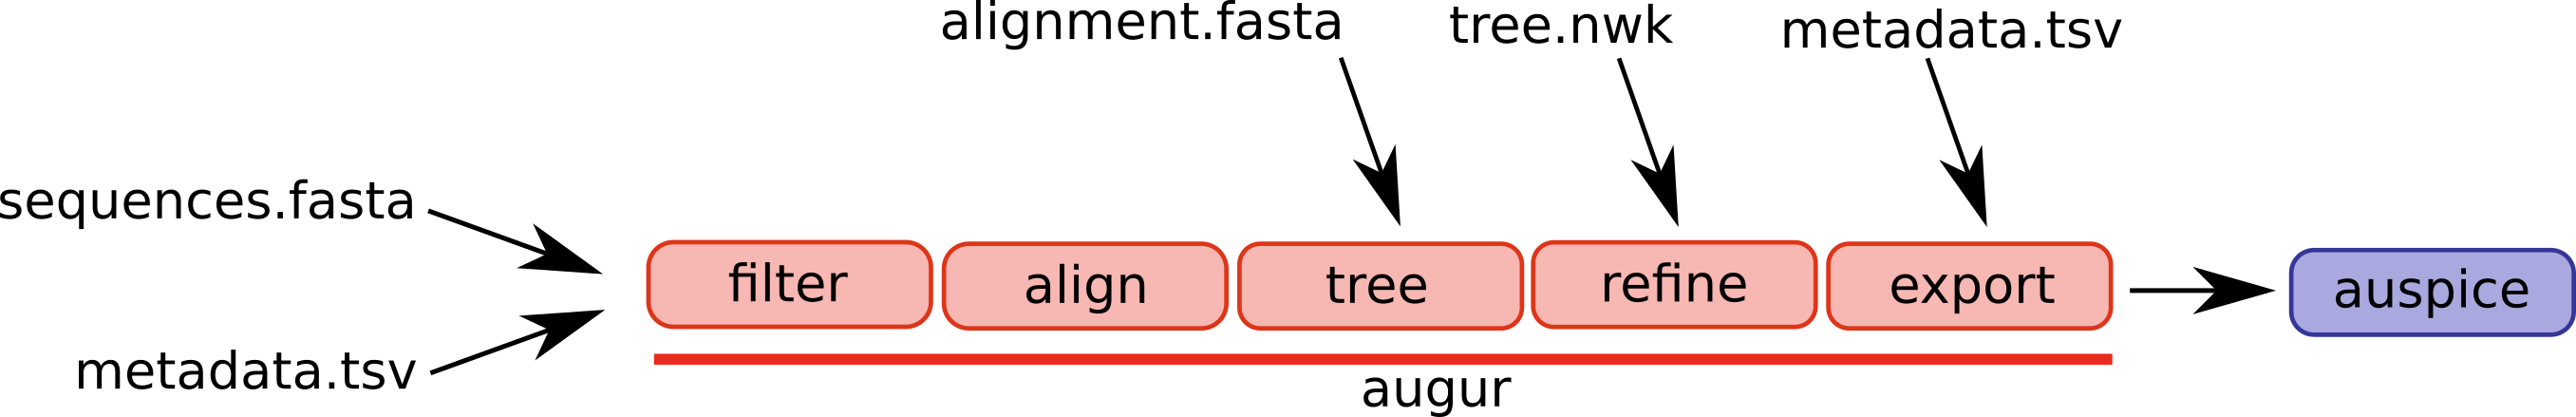
\includegraphics[keepaspectratio]{./img/augur_analysis_sketch.png}}

The steps/functions we use are in this lab are the following:

\begin{itemize}
\tightlist
\item
  \textbf{align}: This step constructs a multiple sequence alignment from this subset of genomes
\item
  \textbf{tree}: This step builds a phylogenetic tree, where branch lengths are measured in substitutions/site (a divergence tree)
\item
  \textbf{refine}: This step constructs a time tree using our existing tree alongside collection dates of SARS-CoV-2 genomic samples (branch lengths are measured in time)
\item
  \textbf{traits}: This step uses treetime's mugration model to infer ancestral traits based on the tree. We will use this to infer ancestral host and geography
\item
  \textbf{export}: This step exports the data to be used by \href{https://auspice.us/}{Auspice}, a version of the visualization system used by NextStrain that lets you examine your own phylogenetic tree and metadata
\end{itemize}

Once these steps are completed, we will spend some time comparing the phylogenetic tree and epidemiological metadata to the results published in the existing study.

\subsubsection{\texorpdfstring{Step 1: Construct a Multiple Sequence Alignment of the Genomes (\texttt{augur\ align})}{Step 1: Construct a Multiple Sequence Alignment of the Genomes (augur align)}}\label{step-1-construct-a-multiple-sequence-alignment-of-the-genomes-augur-align}

The first step is to construct a multiple sequence alignment of the genomes, which is required before building a phylogenetic tree. We will be using the command \texttt{augur\ align} to accomplish this task, but underneath this runs \href{https://mafft.cbrc.jp/alignment/software/}{mafft} to construct the alignment.

To construct the alignment, please run the following:

\textbf{Commands}

\begin{verbatim}
# Time: 10 seconds
augur align --nthreads 2 --sequences data/sequences.fasta --reference-sequence data/reference_MN908947.3.fasta --output alignment.fasta
\end{verbatim}

You should expect to see the following:

\textbf{Output}

\begin{verbatim}
using mafft to align via:
        mafft --reorder --anysymbol --nomemsave --adjustdirection --thread 2 alignment.to_align.fasta 1> alignmnt.fasta 2> alignment.fasta.log

        Katoh et al, Nucleic Acid Research, vol 30, issue 14
        https://doi.org/10.1093%r%2Fgkf436

12bp insertion at ref position 6377
        TGCGTGCGTCGG: hCoV-19/mink/USA/MI-CDC-3886779-001/2020, hCoV-19/mink/USA/MI-CDC-3886954-001/2020, hCoV-19/mink/USA/MI-CDC-3886891-001/2020, hCoV-19/mink/USA/MI-CDC-3886516-001/2020, hCoV-19/Canada/ON-PHL-21-44225/2021, hCoV-19/deer/Canada/ON-WTD-04581-2582/2021, hCoV-19/deer/Canada/ON-WTD-04658-2372/2021, hCoV-19/deer/Canada/ON-WTD-wcov-04662-2575/2021
Trimmed gaps in MN908947.3 from the alignment
\end{verbatim}

The meaning of each parameter:

\begin{itemize}
\tightlist
\item
  \texttt{-\/-nthreads\ 2}: Use 2 threads for the alignment.
\item
  \texttt{-\/-sequences\ data/sequences.fasta}: The input set of sequences in FASTA format.
\item
  \texttt{-\/-output\ alignment.fasta}: The output alignment, in FASTA format.
\item
  \texttt{-\/-reference-sequence\ data/reference\_MN908947.3.fasta}: The reference genome (the Wuhan-Hu 1 genome). This will be included in our alignment and \texttt{augur\ align} will, once the alignment is constructed, remove any insertions with respect to this reference genome (useful when identifying and naming specific mutations later on in the augur pipeline).
\end{itemize}

Once the alignment is complete, you should have a file \texttt{alignment.fasta} in your directory. This is a very similar format as the input file \texttt{sequences.fasta}, but the difference is that sequences have been aligned (possibly by inserting gaps \texttt{-}). This also means that all sequences in \texttt{alignment.fasta} should have the same length (whereas sequences in \texttt{sequences.fasta}, which is not aligned, may have different lengths).

\subsubsection{\texorpdfstring{Step 2: Build a Maximum Liklihood Phylogenetic Tree (\texttt{augur\ tree})}{Step 2: Build a Maximum Liklihood Phylogenetic Tree (augur tree)}}\label{step-2-build-a-maximum-liklihood-phylogenetic-tree-augur-tree}

The next step is to take the set of aligned genomes \texttt{alignment.fasta} and build a phylogenetic tree (a divergence tree). We will use \texttt{augur\ tree} for this, but underneath it (by default) runs \href{http://www.iqtree.org/}{iqtree}, which uses the Maximum Likelihood method (discussed in Module 2) to infer a phylogenetic tree. To build a tree, please run the following:

\textbf{Commands}

\begin{verbatim}
# Time: 15 seconds
augur tree --nthreads 4 --alignment alignment.fasta --output tree.subs.nwk
\end{verbatim}

You should expect to see this (or very similar) output:

\textbf{Output}

\begin{verbatim}
Building a tree via:
        iqtree2 -ntmax 4 -s alignment-delim.fasta -m GTR -ninit 2 -n 2 -me 0.05 -nt AUTO -redo > alignment-delim.iqtree.log
        Nguyen et al: IQ-TREE: A fast and effective stochastic algorithm for estimating maximum likelihood phylogenies.
        Mol. Biol. Evol., 32:268-274. https://doi.org/10.1093/molbev/msu300


Building original tree took 11.159646034240723 seconds
\end{verbatim}

This produces as output a \texttt{tree.subs.nwk} file, which is the actual phylogenetic tree (in Newick format). You can load this file in a variety of phylogenetic tree viewers (such as \url{http://phylo.io/}) but we will further refine this file to work with Auspice.

Another output file is \texttt{alignment-delim.iqtree.log}, which contains additional information from iqtree. You can take a look at this file to get an idea of what \href{http://www.iqtree.org/}{iqtree} was doing by using \texttt{tail} (prints the last few lines of a file).

\textbf{Commands}

\begin{verbatim}
tail -n 20 alignment-delim.fasta.log
\end{verbatim}

\textbf{Output}

\begin{verbatim}
Optimal log-likelihood: -42013.225
Rate parameters:  A-C: 0.16166  A-G: 0.97768  A-T: 0.06332  C-G: 0.00010  C-T: 6.44146  G-T: 1.00000
Base frequencies:  A: 0.299  C: 0.183  G: 0.197  T: 0.322
Parameters optimization took 1 rounds (0.006 sec)
BEST SCORE FOUND : -42013.225
Total tree length: 0.006

Total number of iterations: 2
CPU time used for tree search: 0.083 sec (0h:0m:0s)
Wall-clock time used for tree search: 0.043 sec (0h:0m:0s)
Total CPU time used: 20.087 sec (0h:0m:20s)
Total wall-clock time used: 11.073 sec (0h:0m:11s)

Analysis results written to:
  IQ-TREE report:                alignment-delim.fasta.iqtree
  Maximum-likelihood tree:       alignment-delim.fasta.treefile
  Likelihood distances:          alignment-delim.fasta.mldist
  Screen log file:               alignment-delim.fasta.log
\end{verbatim}

As iqtree uses a Maximum Likelihood approach, you will see that it will report the likeihood score of the optimal tree (reported as log-likehoods since likelihood values are very very small).

For this lab we are not looking at branch support values for a tree, but for real-world analysis you may wish to look into including bootstrap support values or approximate likelihood ratio test values. This will give a measure of how well supported each branch in the tree is by the alignment (often a number from 0 for little support to 100 for maximal support). Please see the IQTree documentation for more details.

\subsubsection{\texorpdfstring{Step 3: Inferring Timing of Host Change (\texttt{augur\ refine})}{Step 3: Inferring Timing of Host Change (augur refine)}}\label{step-3-inferring-timing-of-host-change-augur-refine}

The tree output by \href{http://www.iqtree.org/}{iqtree} shows hypothetical evolutionary relationships between different SARS-CoV-2 genomes with branch lengths representing distances between different genomes (in units of \textbf{substitutions/site} i.e., the predicted number of substitutions between genomes divided by the alignment length). However, other methods of measuring distance between genomes are possible. In particular we can incorporate the collection dates of the different SARS-CoV-2 genomes to infer a tree where branches are scaled according to the elapsed time and the dates of internal nodes are inferred. Such trees are called \textbf{time trees}.

We will use \href{https://treetime.readthedocs.io/en/latest/}{TreeTime} to infer a \textbf{time tree} from our phylogenetic tree using collection dates of the SARS-CoV-2 genomes stored in the \texttt{metadata.tsv} metadata file. We will use the \texttt{augur\ refine} step to run TreeTime and perform some additional refinemint of the tree. To do this, please run the following:

\textbf{Commands}

\begin{verbatim}
# Time: 5 minutes
augur refine --alignment alignment.fasta --tree tree.subs.nwk --metadata data/metadata.tsv --timetree --divergence-units
mutations --output-tree tree.time.nwk --output-node-data refine.node.json --keep-root
\end{verbatim}

You should expect to see the following as output:

\textbf{Output}

\begin{verbatim}
augur refine is using TreeTime version 0.9.4

21.73   WARNING: Previous versions of TreeTime (<0.7.0) RECONSTRUCTED sequences of
        tips at positions with AMBIGUOUS bases. This resulted in unexpected
        behavior is some cases and is no longer done by default. If you want to
        replace those ambiguous sites with their most likely state, rerun with
        `reconstruct_tip_states=True` or `--reconstruct-tip-states`.
[...]

Inferred a time resolved phylogeny using TreeTime:
        Sagulenko et al. TreeTime: Maximum-likelihood phylodynamic analysis
        Virus Evolution, vol 4, https://academic.oup.com/ve/article/4/1/vex042/4794731

updated tree written to tree.time.nwk
node attributes written to refine.node.json
\end{verbatim}

The parameters we used are:

\begin{itemize}
\tightlist
\item
  \texttt{-\/-alignment\ alignment.fasta}: The alignment used to build the tree. Used to re-scale the divergence units.
\item
  --tree tree.subs.nwk: The input tree build using iqtree.
\item
  --metadata data/metadata.tsv: The metadata which contains the SARS-CoV-2 genome names (in a column called strain) and the sample collection dates (in a column named date).
\item
  --timetree: Build a time tree.
\item
  --divergence-units mutations: Convert the branch lengths of substitutions/site (mutations/site) to mutations (not needed to build a time tree, this is just used for visualizing the tree later on).
\item
  --output-tree tree.time.nwk: The output Newick file containing the time tree.
\item
  --output-node-data refine.node.json: Augur will store additional information here which will let us convert between time trees and substitution trees.
\item
  --keep-root: Keep the reference genome as the root
\end{itemize}

As output, the file \texttt{tree.time.nwk} will contain the time tree while the file \texttt{refine.node.json} contains additional information about the tree. The tree \texttt{tree.time.nwk} will also be rooted based on analysis performed by \href{https://treetime.readthedocs.io/en/latest/}{TreeTime}.

\subsubsection{Step 4: Infer Ancestral States for Host and Location}\label{step-4-infer-ancestral-states-for-host-and-location}

We will now be using treetime's \texttt{mugration} model to reconstruct ancestral trait states. In other words, we are trying to use the tree and genome metadata to reconstruct the most likely host and location (the state/province stored as \texttt{division} in data/metadata.tsv) at each of the internal nodes in the tree. As with the other analyses, augur makes this process very convenient:

\textbf{Commands}

\begin{verbatim}
# Time: 1 minute
augur traits --tree tree.time.nwk --metadata data/metadata.tsv --columns host division --output-node-data trait.node.json
\end{verbatim}

You should expect to see the following as output:

\textbf{Output}

\begin{verbatim}
augur traits is using TreeTime version 0.9.4
Assigned discrete traits to 31 out of 35 taxa.

NOTE: previous versions (<0.7.0) of this command made a 'short-branch
length assumption. TreeTime now optimizes the overall rate numerically
and thus allows for long branches along which multiple changes
accumulated. This is expected to affect estimates of the overall rate
while leaving the relative rates mostly unchanged.
Assigned discrete traits to 31 out of 35 taxa.

[...]

Inferred ancestral states of discrete character using TreeTime:
        Sagulenko et al. TreeTime: Maximum-likelihood phylodynamic analysis
        Virus Evolution, vol 4, https://academic.oup.com/ve/article/4/1/vex042/4794731

results written to trait.node.json
\end{verbatim}

The parameters we used are:

\begin{itemize}
\tightlist
\item
  \texttt{-\/-tree\ tree.time.nwk}: The time-calibrated tree we inferred in step 4
\item
  \texttt{-\/-metadata\ data/metadata.tsv}: The metadata file with information about the genomes in the tree
\item
  \texttt{-\/-columns\ host\ division}: The columns in the metadata file we want to infer ancestral states for, in this case host (what species the genome came from) and division (the province/state the genome came from).
\item
  \texttt{-\/-output-node-data\ trait.node.json}: Augur stores the additional information related to the ancestral trait inference for later visualisation.
\end{itemize}

\subsubsection{\texorpdfstring{Step 5: Package up data for Auspice Visualisation (\texttt{augur\ export})}{Step 5: Package up data for Auspice Visualisation (augur export)}}\label{step-5-package-up-data-for-auspice-visualisation-augur-export}

We will be using \href{https://auspice.us/}{Auspice} to visualize the tree alongside our metadata. To do this, we need to package up all of the data we have so far into a special file which can be used by Auspice. To do this, please run the following command:

\textbf{Commands}

\begin{verbatim}
# Time: 1 second
augur export v2 --tree tree.time.nwk --node-data refine.node.json trait.node.json --maintainers "CBW-IDE-2024" --title "Module 8 Practical" --output analysis-package.json --geo-resolutions division
\end{verbatim}

You should expect to see the following as output:

\textbf{Output}

\begin{verbatim}
Trait 'host' was guessed as being type 'categorical'. Use a 'config' file if you'd like to set this yourself.
Trait 'division' was guessed as being type 'categorical'. Use a 'config' file if you'd like to set this yourself.
Validating produced JSON
Validating schema of 'analysis-package.json'...
Validating that the JSON is internally consistent...
Validation of 'analysis-package.json' succeeded.
\end{verbatim}

The file \texttt{analysis-package.json} contains the tree with different branch length units (time and sustitutions), our inferred ancestral traits, as well as additional data.

The parameters we used are:

\begin{itemize}
\tightlist
\item
  \texttt{-\/-tree\ tree.time.nwk}: The time-calibrated tree we inferred in step 4
\item
  \texttt{-\/-node-data\ refine.node.json\ trait.node.json}: The 2 jsons created during the temporal and ancestral trait inference
\item
  \texttt{-\/-title\ "Module\ 8\ Practical"}: A title for the auspice page, you can make this anything you want.
\item
  -\texttt{-maintainers\ "CBW-IDE-2024"}: A name for who is responsible for this analysis, useful for later, can make this anything you want.
\item
  \texttt{-\/-geo-resolutions\ division}: Spatial resolution on which to plot the data. In this case we want province/state i.e., division
\item
  \texttt{-\/-output\ analysis-package.json}: The key output file we want to generate
\end{itemize}

\subsection{5. Visualizing the Phylodynamic Analysis Alongside Epidemiological Metadata}\label{visualizing-the-phylodynamic-analysis-alongside-epidemiological-metadata}

Now that we've constructed and packaged up a tree (\texttt{analysis-package.json}), we can visualize this data alongside the data augur has we've extracted from our metadata using augur (\texttt{data/metadata.tsv}) using \href{https://auspice.us/}{Auspice}.

I've had issues recently getting this to work in firefox so recommend using a chromium-based browser if you have issues.

\subsubsection{Step 1: Load Data into Auspice}\label{step-1-load-data-into-auspice}

To do this, please navigate to \url{http://IP-ADDRESS/module8/} and download the files \texttt{analysis-package.json} and \texttt{data/metadata.tsv} to your computer (if the link does not download you can \textbf{Right-click} and select \textbf{Save link as\ldots{}}).

Next, navigate to \url{https://auspice.us/} and drag the file \texttt{analysis-package.json} onto the page.

\pandocbounded{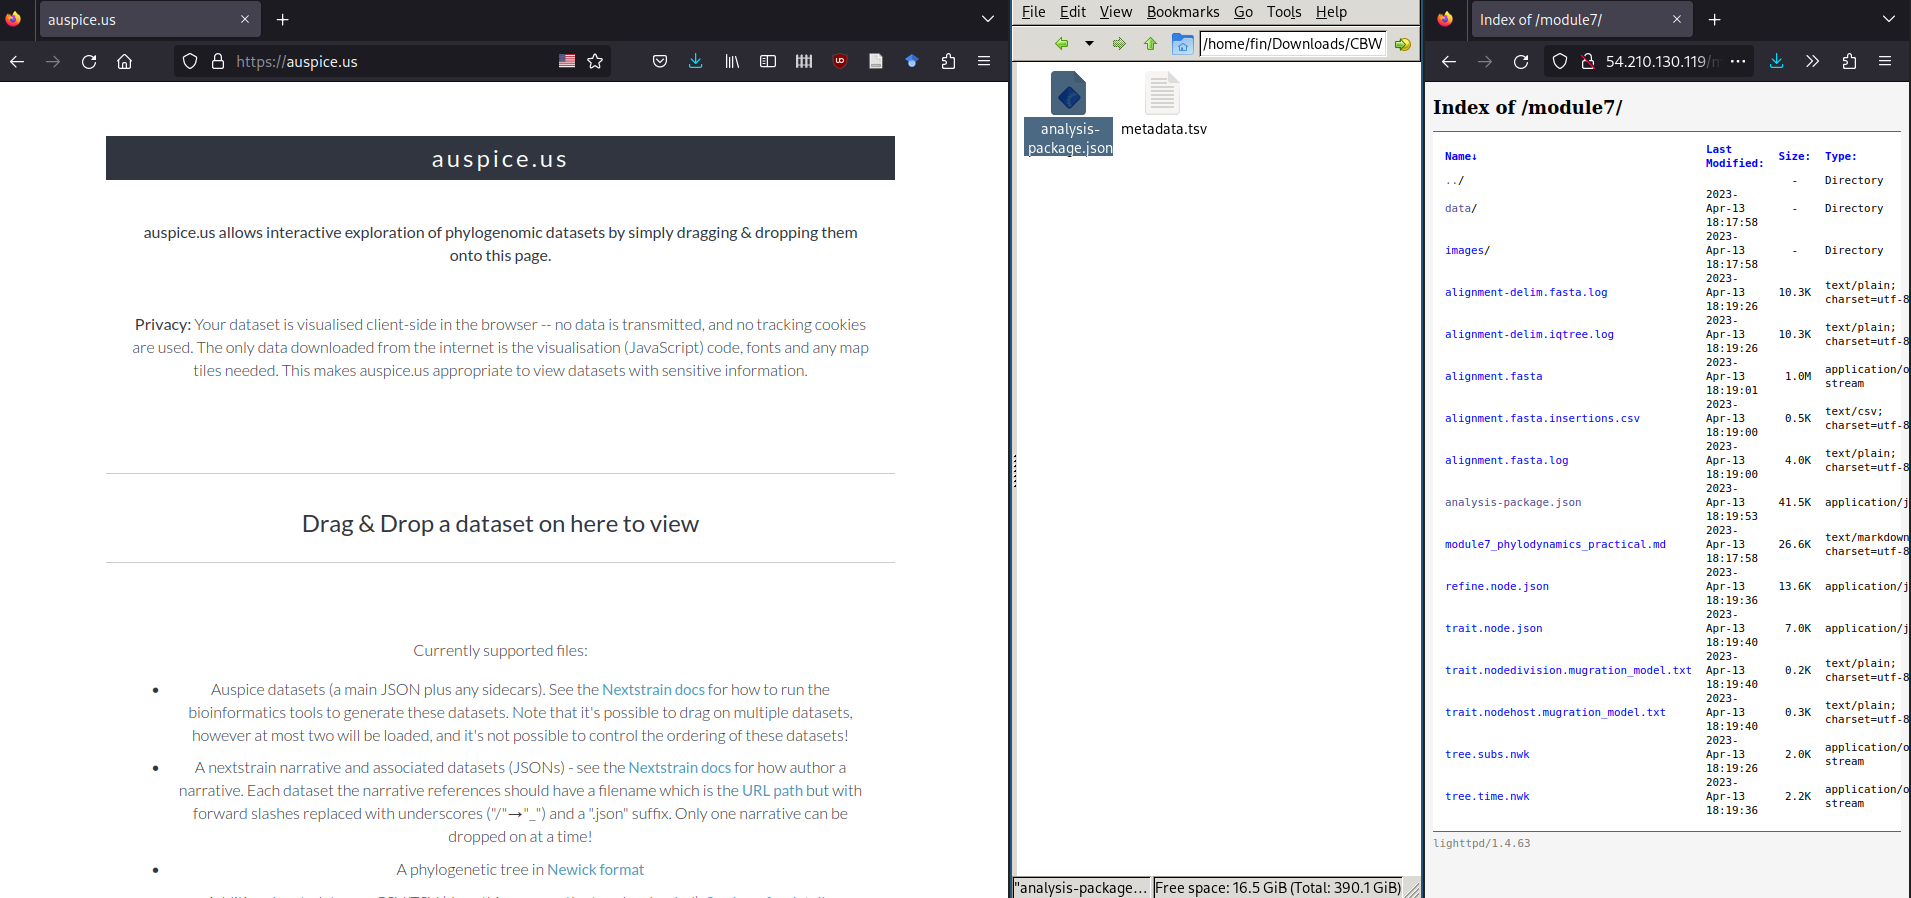
\includegraphics[keepaspectratio]{./img/auspice.png}}

This should result in a phylogenetic tree being loaded that looks like:

\pandocbounded{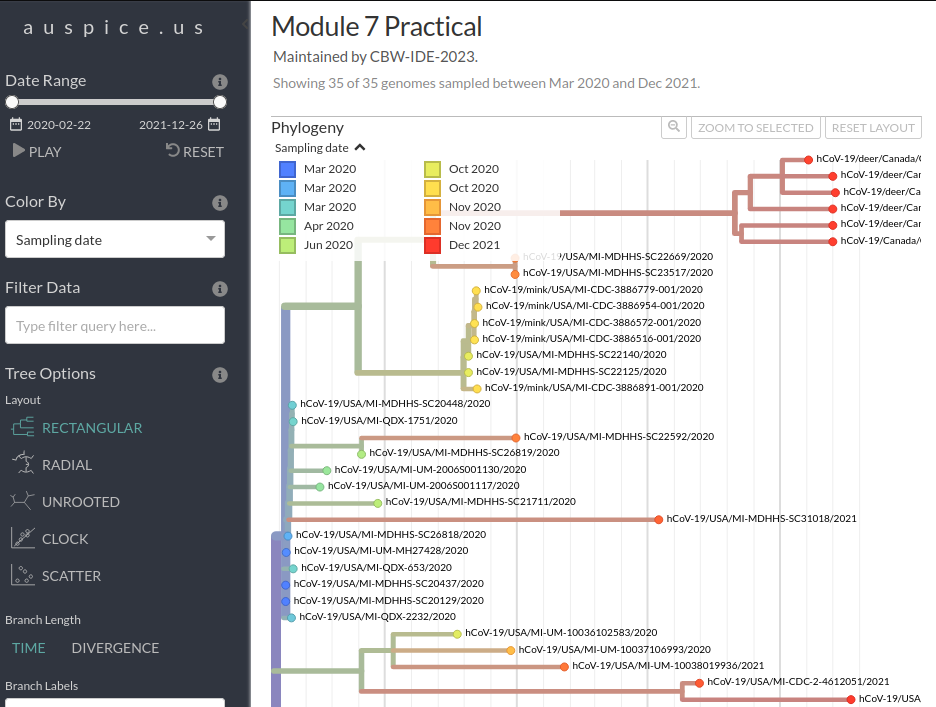
\includegraphics[keepaspectratio]{./img/tree.png}}

Next, we will load the metadata \texttt{data/metadata.tsv} file onto this view. To do this, please find and drag-and-drop the \texttt{data/metadata.tsv} file onto the phylogenetic tree shown in Auspice:

\pandocbounded{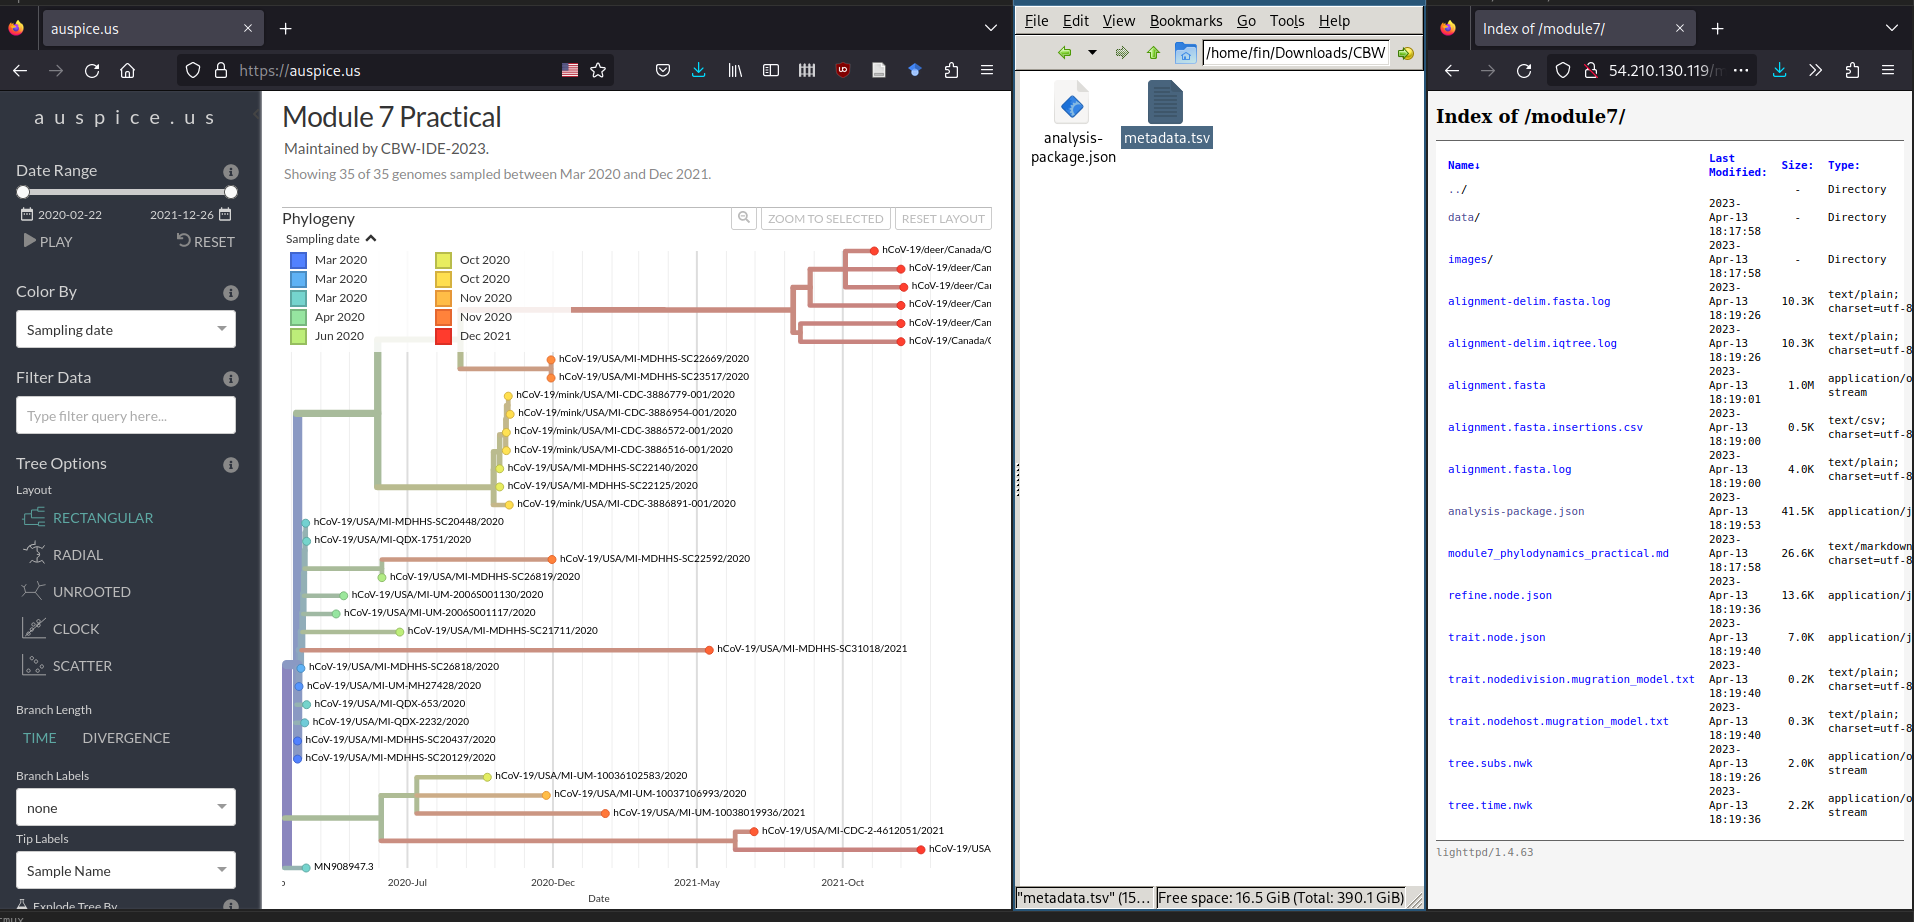
\includegraphics[keepaspectratio]{./img/metadata.png}}

You may get some warning messages showing up, but you should still see a green \textbf{Added metadata from metadata.tsv} message.

\pandocbounded{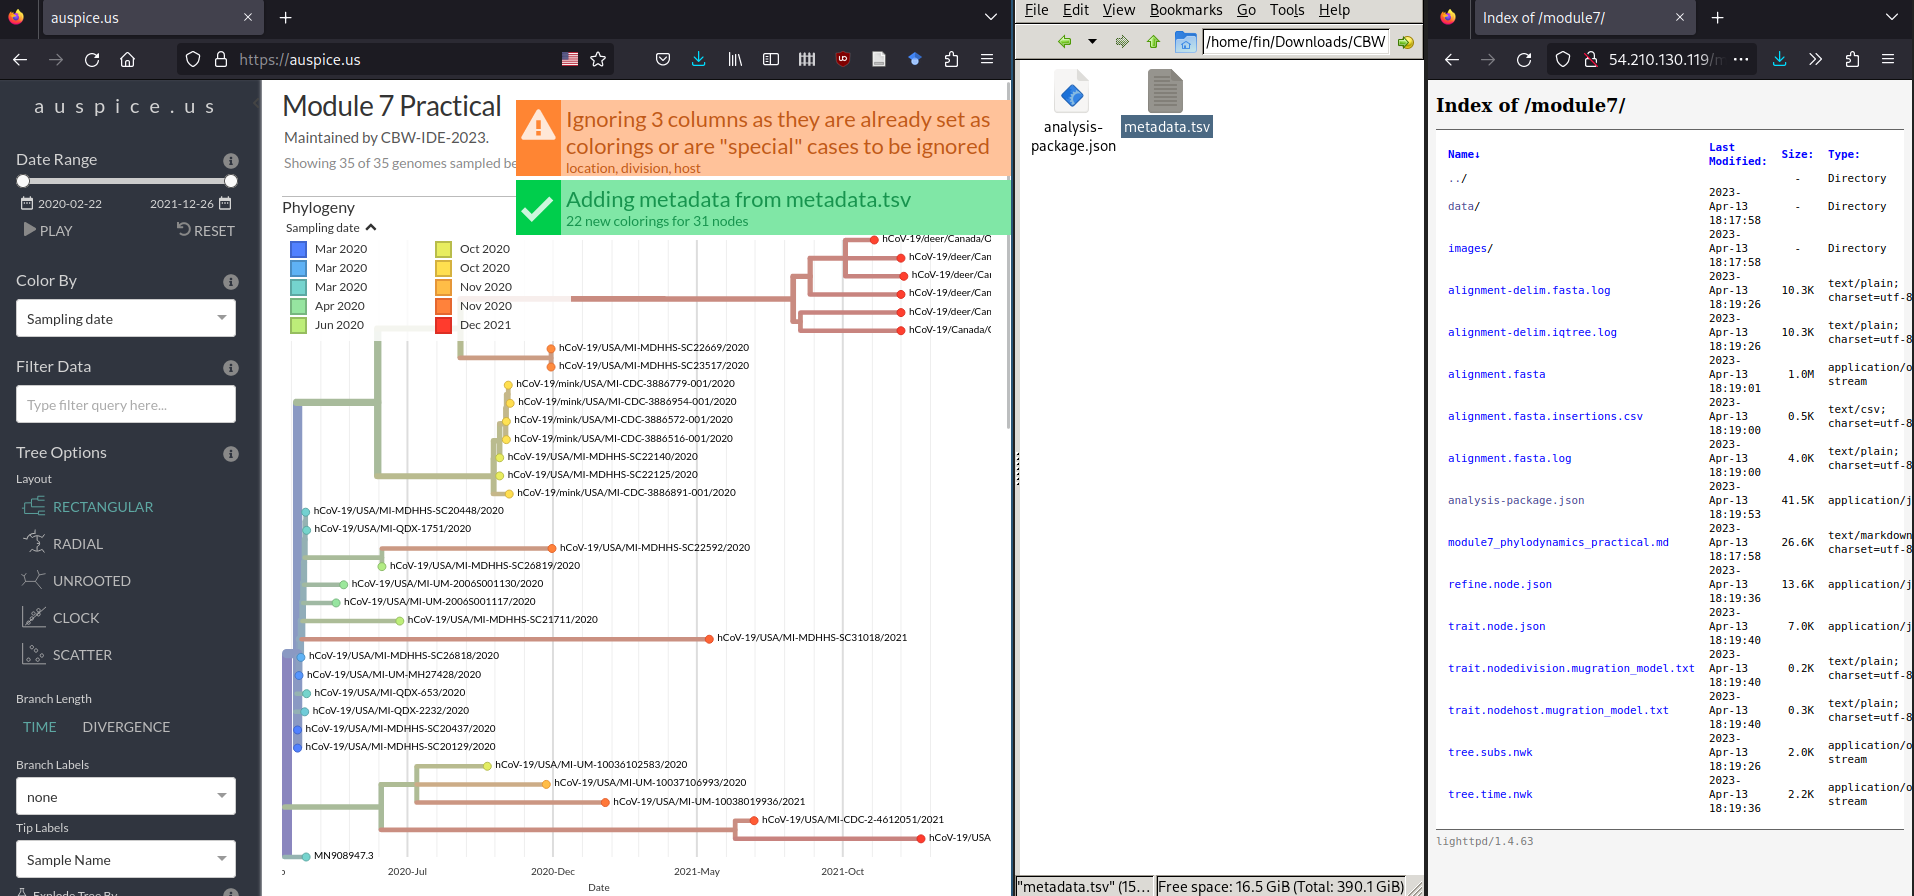
\includegraphics[keepaspectratio]{./img/metadata2.png}}

\subsubsection{Step 2: Explore Data}\label{step-2-explore-data}

Now you can spend some time to explore the data and get used to the Auspice interface. Try switching between different \textbf{Tree Layouts}, or different \textbf{Branch Lengths}, or colouring the tree by different criteria in the metadata table. This is always worth doing a bit before diving into analyses!

\subsubsection{Step 3: Examine the Molecular Clock Analysis}\label{step-3-examine-the-molecular-clock-analysis}

Now we are going to look more at the Branch length ``TIME'' and ``DIVERGENCE'' options as well as the ``CLOCK'' layout/figure found in the options bar on the left of your screen.

\pandocbounded{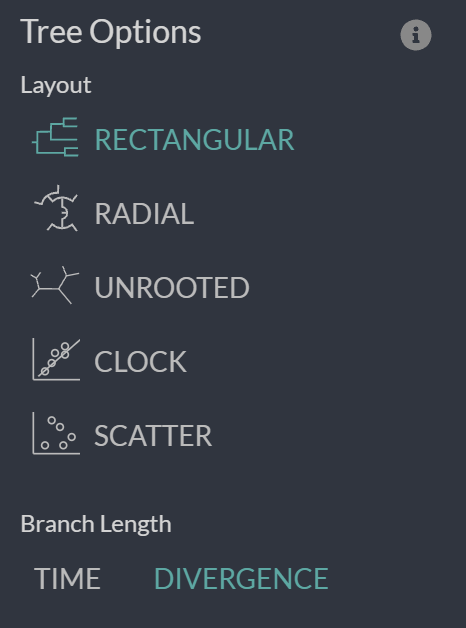
\includegraphics[keepaspectratio]{./img/auspice-panel.png}}

First, let's look at the divergence tree and use the x-axis to work out how many mutations there are on certain branches. We can use the x-axis in the ``RECTANGULAR'' layout of the ``DIVERGENCE'' tree to work this out or we can directly move our cursor over the node/branch of interest to have a pop-up with the details.

\pandocbounded{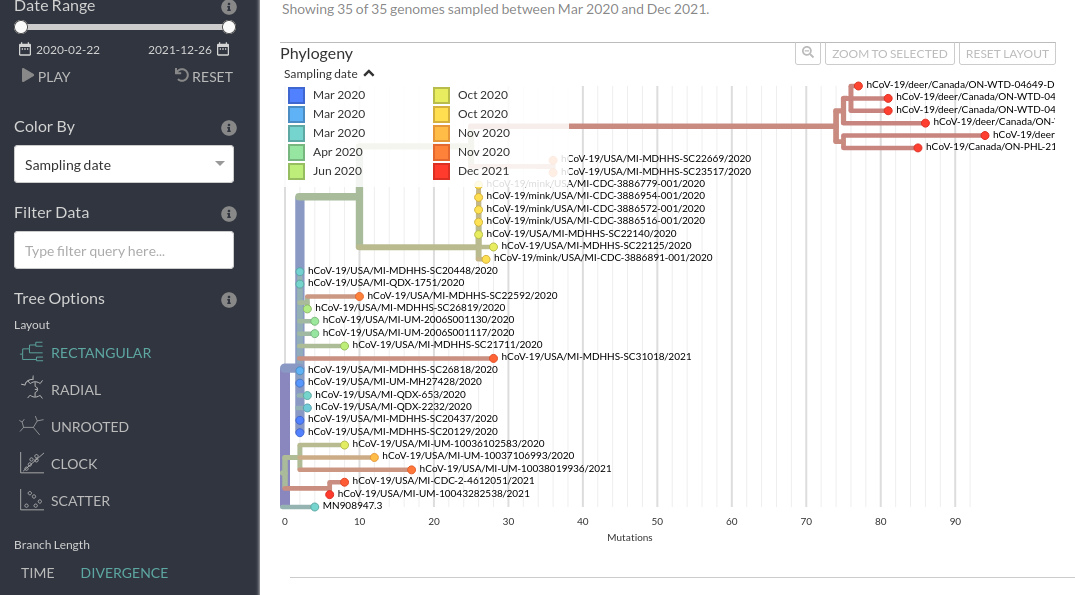
\includegraphics[keepaspectratio]{./img/divergence.png}}

Now, we can do the same thing if we switch to ``TIME'' and look at the approximate inferred dates of the internal nodes of the tree. We can also mouse over to get the exact pop-up dates.

\pandocbounded{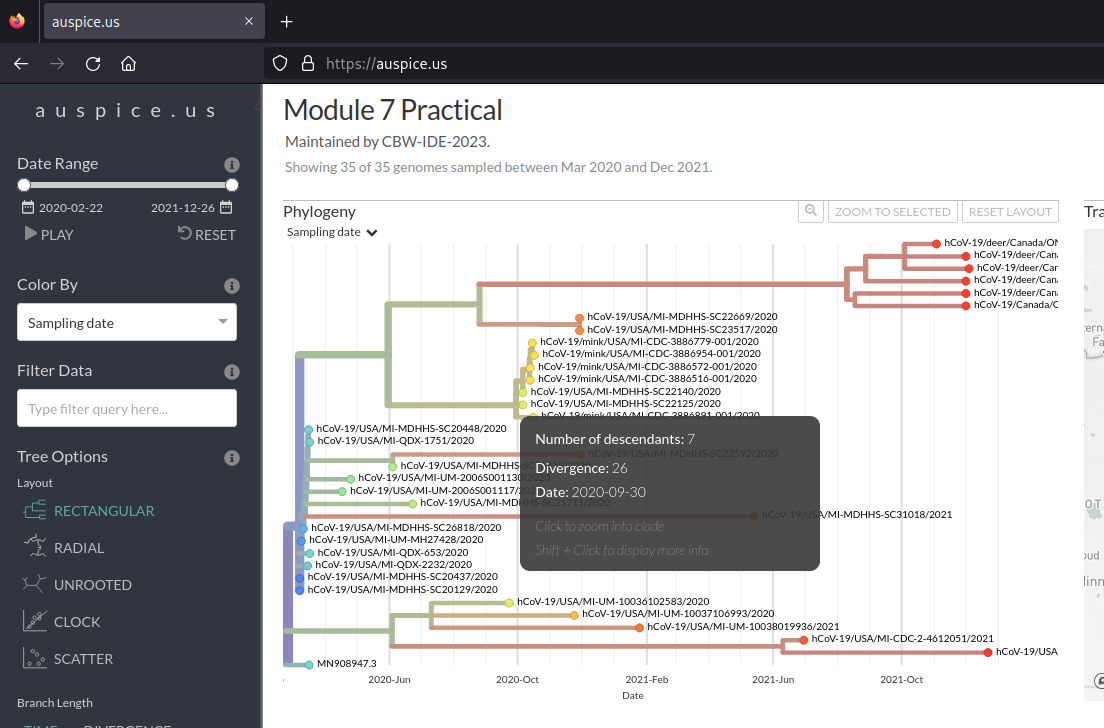
\includegraphics[keepaspectratio]{./img/date.png}}

Finally, we can look at the tip-to-root regression from the divergence tree (i.e., how long each genome's total branch length in mutations is all the way to root vs the collection date). This can be done by selecting ``DIVERGENCE'' under the ``Branch Length'' header.

\pandocbounded{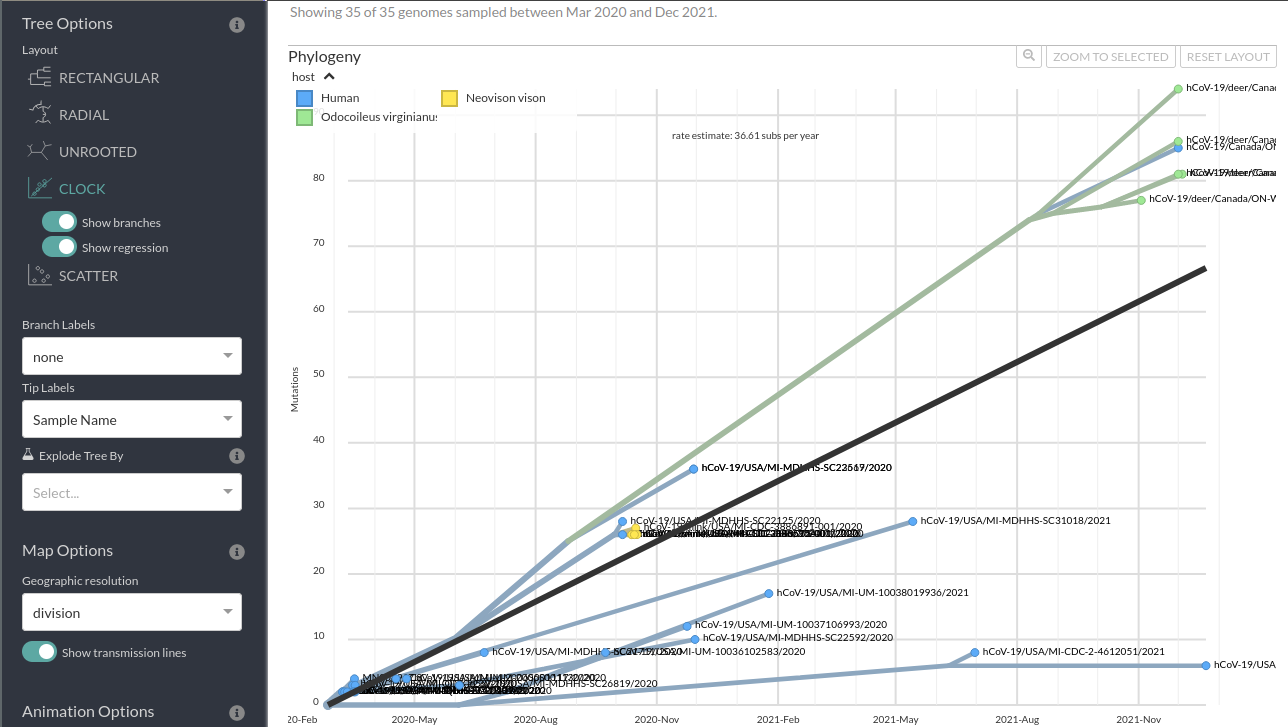
\includegraphics[keepaspectratio]{./img/tip_reg.png}}

\subsubsection{Step 3: Questions}\label{step-3-questions}

\begin{enumerate}
\def\labelenumi{\arabic{enumi}.}
\tightlist
\item
  When was the last common ancestor of the ON Deer clade?
\item
  What about the last common ancestor of this clade and the nearest other sequences?
\item
  Does the trend line for the molecular clock (tip-to-root regression) look a good fit? Do you think there may be more than 1 mutation rate in these samples?
\item
  Given the amount of data and your answer to 1, how accurate do you think the inferred node date is?
\item
  How might you represent the degree of certainty or uncertainty in these estimates?
\end{enumerate}

\subsubsection{Step 4: Examine the Ancestral Trait Inference}\label{step-4-examine-the-ancestral-trait-inference}

We can colour the tree and rename the tree tip labels using the metadata to infer ancestral traits. The internal nodes/branches will be coloured based on the inferred ancestral state.

For example, you can look at the inferred ancestral host information using these options:

\pandocbounded{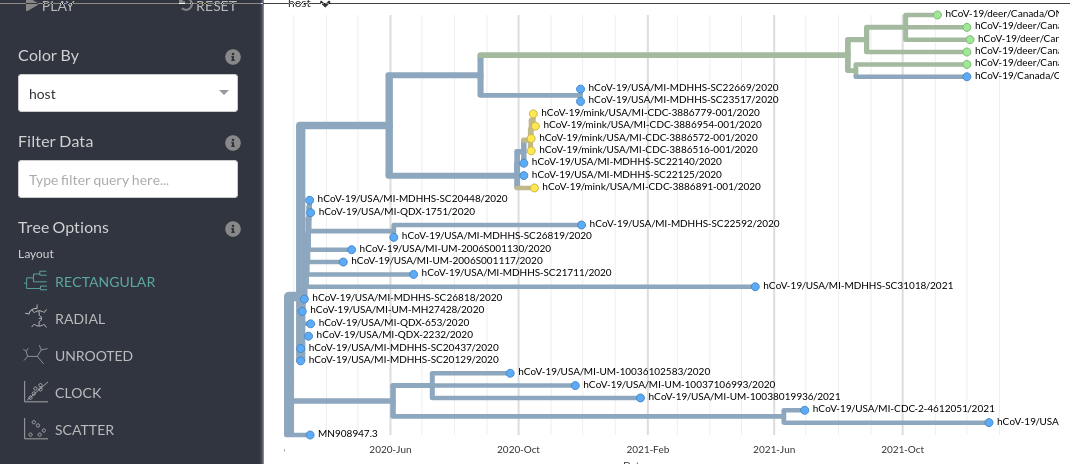
\includegraphics[keepaspectratio]{./img/host.png}}

Similarly, you can look at the inferred ancestral location information using these options:

\pandocbounded{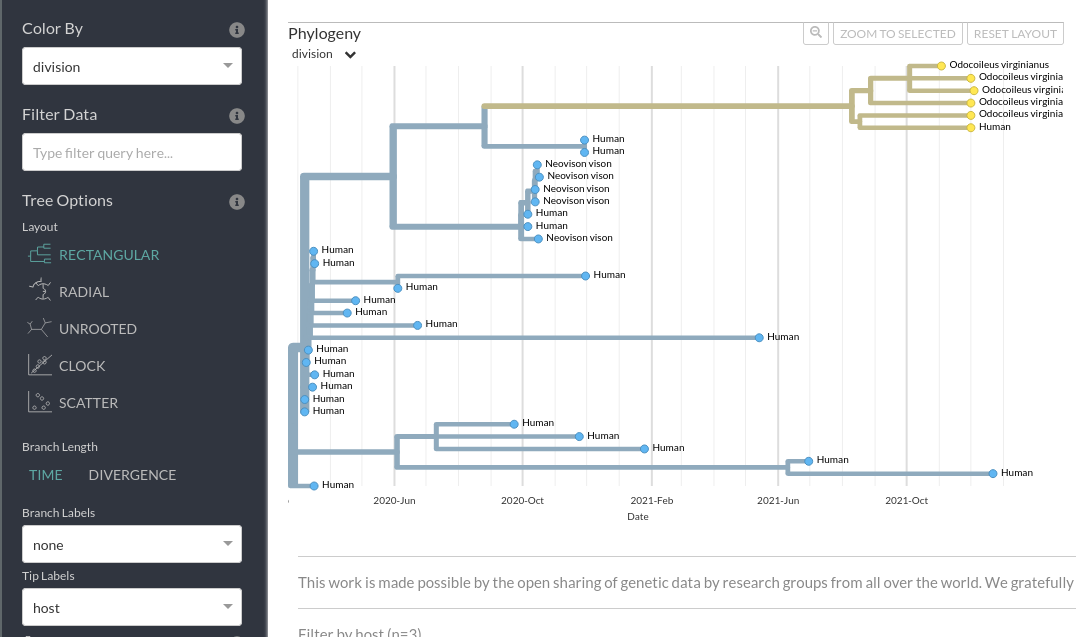
\includegraphics[keepaspectratio]{./img/loc.png}}

\subsubsection{Step 4: Questions}\label{step-4-questions}

\begin{enumerate}
\def\labelenumi{\arabic{enumi}.}
\tightlist
\item
  Based on this analysis was the common ancestor of the ON Deer+Human clade inferred to have been in a human or in a deer?
\item
  What about the common ancestor of the wider ON Deer+Human, MI Mink+Human clades?
\item
  Why might this analysis be misleading?
\item
  Where is the ON Deer+Human clade inferred to have originated: Ontario or Michigan?
\end{enumerate}

\subsection{6. Selection Analysis}\label{selection-analysis}

Now we are going to try and do a selection analysis. In particular, we are going to use some of the models in hyphy to determine whether the dN/dS (also known as ω) ratio (ratio of non-synonymous mutations per non-synonymous site to synonymous mutation per synonymous site) is significantly different in the ON Deer+Human clade than the rest of our dataset.

To do this we first need an alignment that captures information about dN/dS i.e., a codon alignment. To be honest, these are fairly irritating to generate. The classic tool \href{http://www.bork.embl.de/pal2nal/\#RunP2N}{PAL2NAL} or \href{https://github.com/veg/hyphy-analyses/blob/master/codon-msa/README.md}{hyphy's own method} needs us to have an alignment of a given gene (dN and dS only make sense for coding sequences) in both protein and nucleotide form. This can often require custom sequence manipulation and is sensitive to sequences with errors or unresolved regions.

For this exercise, we are going to generate a codon alignment for the S using a tool called virulign

\textbf{Commands}

\begin{verbatim}
# Time: 5 minutes
./code/virulign data/S.xml data/sequences.fasta --exportAlphabet Nucleotides --exportKind GlobalAlignment --exportReferenceSequence yes --progress yes > S_codon_alignment.fasta
\end{verbatim}

Then as you did previously, you want to download \texttt{S\_codon\_alignment.fasta} by navigating to \url{http://IP-ADDRESS/module8/} (or using scp if you are familiar with it). Once you've got the codon alignment, we are going to go the \href{https://www.datamonkey.org/}{datamonkey.org} website. This is very useful webserver that is provided by the authors of hyphy to make it easier to use their methods. As you can see on the home page there is even a nice wizard that will guide you towards the correct model for the analysis you want to perform.

In this case we are interested in \emph{selection} across \emph{branches} of the \emph{episodic} kind which will guide us towards a method called \href{https://www.datamonkey.org/absrel}{aBSREL (adaptive Branch-Site RandomEffects Likelihood)}.

\pandocbounded{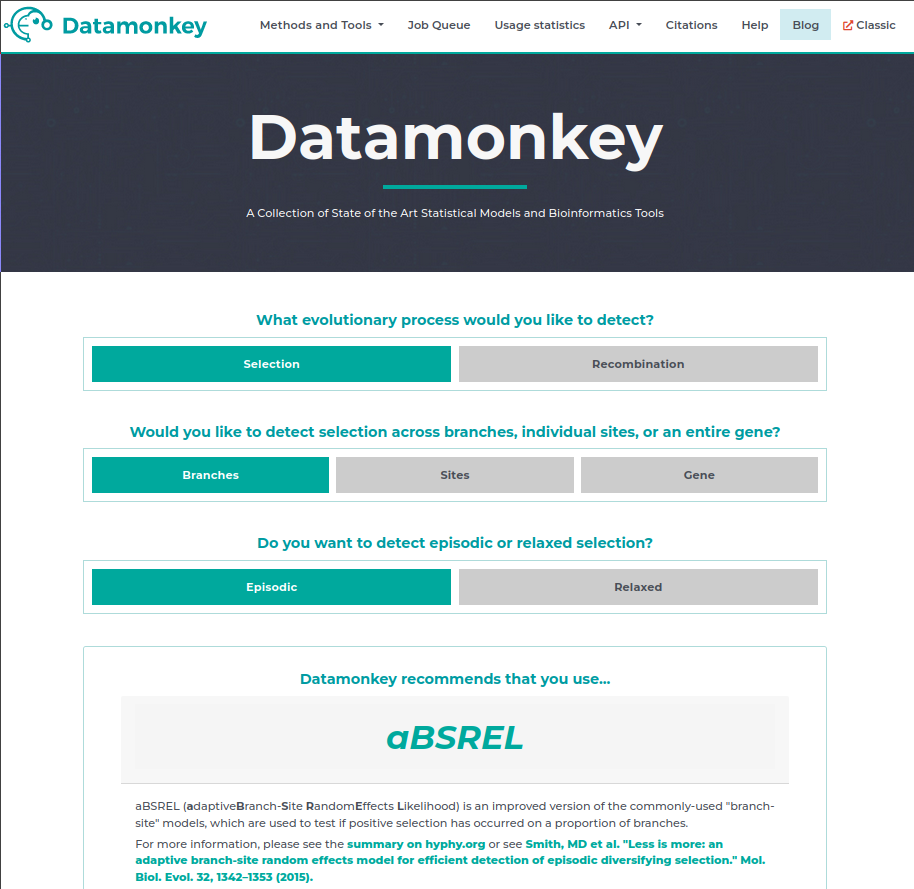
\includegraphics[keepaspectratio]{./img/absrel.png}}

We are going to follow the instructions on the page and select our \texttt{S\_codon\_alignment.fasta} as input, enter our email address (just in case), then hit \texttt{run\ analysis}.

\pandocbounded{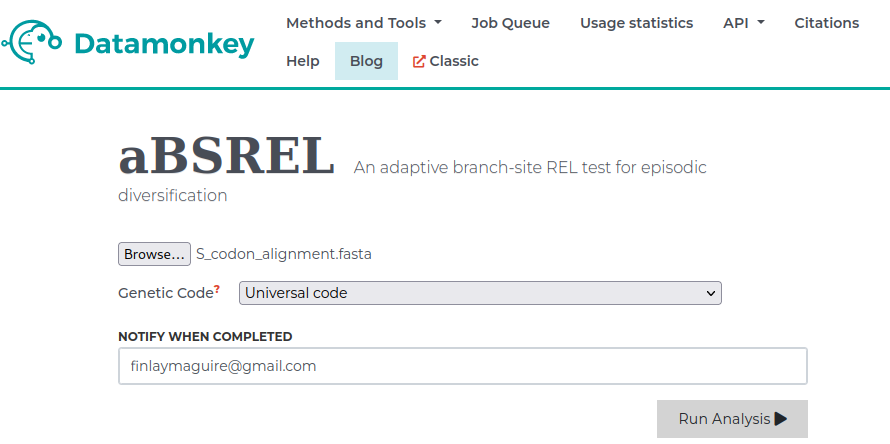
\includegraphics[keepaspectratio]{./img/absrel2.png}}

This will take us to a new page where we can select the branches we want to test for increased episodic selection relative to the rest of the tree. In this case we are interested in the ON Deer+Human clade so we will select those branches. Then we will hit \texttt{Save\ Branch\ Selection} and begin running our analysis.

\pandocbounded{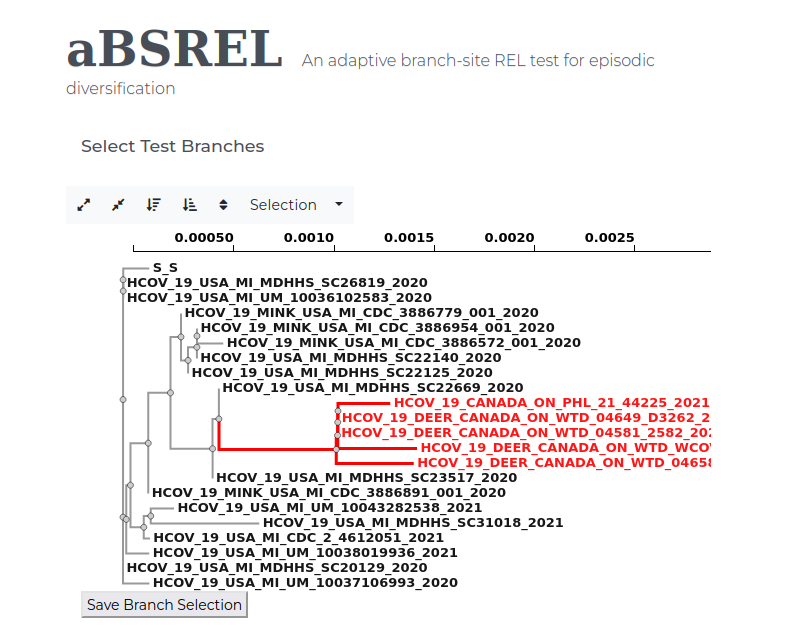
\includegraphics[keepaspectratio]{./img/select_all.png}}

If all goes well this will run for a minute or two (depending on server load) before directing us to an nice results page with lots of details.

\pandocbounded{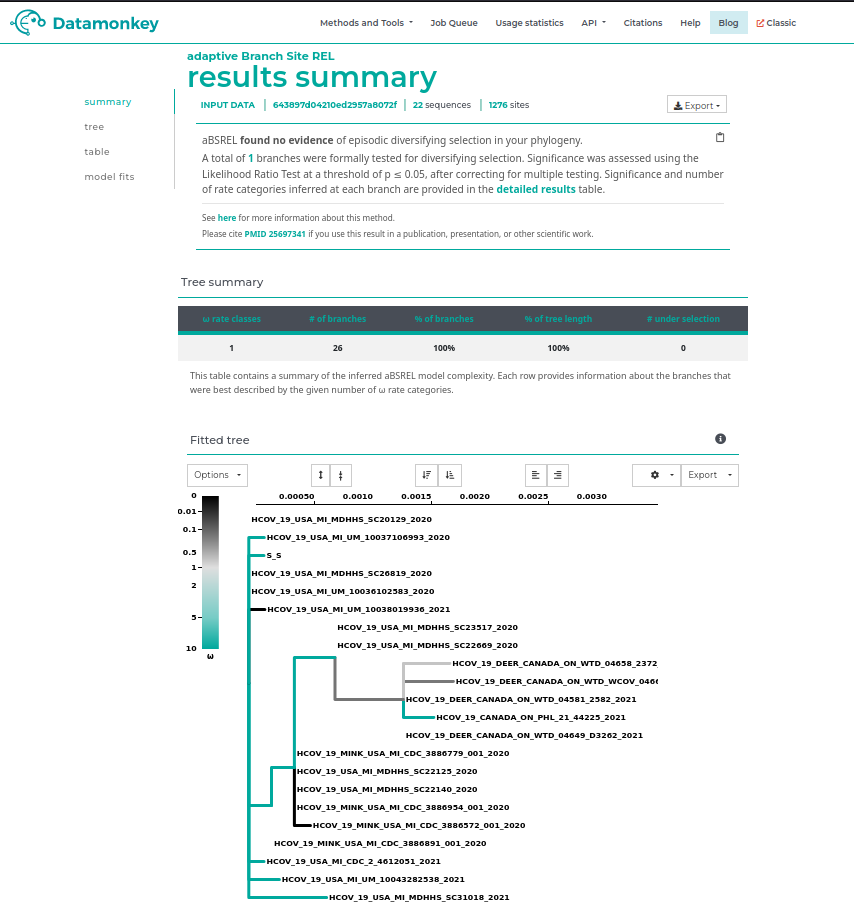
\includegraphics[keepaspectratio]{./img/results.png}}

\subsubsection{Questions}\label{questions}

\begin{enumerate}
\def\labelenumi{\arabic{enumi}.}
\tightlist
\item
  At the top of the page there is a summary of the result, is there any sign of increased episodic selection in this clade?
\item
  Look at the fitted tree output below, based on the colorbar in the legend for values of ω (dN/dS), is the inferred ω \textgreater{} 1 or \textless{} 1 in the branches leading up to the ON Deer+Human clade?
\item
  What might this represent in terms of the differences between deer and human immune responses?
\item
  Can you think of any limitations of this analysis?
\end{enumerate}

Congratulations! You have completed Lab 7!

\chapter{Module 8: Emerging Pathogen Detection and Identification}\label{module-8-emerging-pathogen-detection-and-identification}

\section{Lecture}\label{lecture-7}

\subsection{1. Introduction}\label{introduction-3}

This tutorial aims to introduce a variety of software and concepts related to detecting emerging pathogens from a complex host sample. The provided data and methods are derived from real-world data, but have been modified to either illustrate a specific learning objective or to reduce the complexity of the problem. Contamination and a lack of large and accurate databases render detection of microbial pathogens difficult. As a disclaimer, all results produced from the tools described in this tutorial and others must also be verified with supplementary bioinformatics or wet-laboratory techniques.

\subsection{2. List fo Software for Tutorial and its Respective Documentation}\label{list-fo-software-for-tutorial-and-its-respective-documentation}

\begin{itemize}
\tightlist
\item
  \href{https://github.com/OpenGene/fastp}{fastp}
\item
  \href{https://multiqc.info/}{multiqc}
\item
  \href{https://kat.readthedocs.io/en/latest/}{KAT}
\item
  \href{https://ccb.jhu.edu/software/kraken2/}{Kraken2}
\item
  \href{https://fbreitwieser.shinyapps.io/pavian/}{Pavian}
\item
  \href{https://github.com/voutcn/megahit}{MEGAHIT}
\item
  \href{http://quast.sourceforge.net/quast}{Quast}
\item
  \href{https://blast.ncbi.nlm.nih.gov/Blast.cgi}{NCBI blast}
\end{itemize}

The workshop machines already have this software installed within a conda environment, but to perform this analysis later on, you can make use of the conda environment located at \href{https://bioinformaticsdotca.github.io/IDE_2024/module10/environment.yml}{environment.yml} to install the necessary software.

\subsection{3. Exercise Setup}\label{exercise-setup-1}

\subsubsection{3.1. Copy Data Files}\label{copy-data-files-1}

To begin, we will copy over the exercises to \texttt{\textasciitilde{}/workspace}. This let's use view the resulting output files in a web browser.

\textbf{Commands}

\begin{verbatim}
cp -r ~/CourseData/IDE_data/module10/module10_workspace/ ~/workspace/
cd ~/workspace/module10_workspace/analysis
\end{verbatim}

When you are finished with these steps you should be inside the directory \texttt{/home/ubuntu/workspace/module10\_workspace/analysis}. You can verify this by running the command \texttt{pwd}.

\textbf{Output after running} \texttt{pwd}

\begin{verbatim}
/home/ubuntu/workspace/module10_workspace/analysis
\end{verbatim}

You should also have a directory like \texttt{data}/ one directory up from here. To check this, you can run \texttt{ls\ ../}:

\textbf{Output after running} \texttt{ls\ ../}

\begin{verbatim}
analysis  data  precomputed-analysis
\end{verbatim}

\subsubsection{3.2. Activate Environment}\label{activate-environment-1}

Next we will activate the \href{https://docs.conda.io/en/latest/}{conda} environment, which will have all the tools needed by this tutorial pre-installed. To do this please run the following:

\textbf{Commands}

\begin{verbatim}
conda activate module10-emerging-pathogen
\end{verbatim}

You should see the command-prompt (where you type commands) switch to include \texttt{(module10-emerging-pathogen)} at the beginning, showing you are inside this environment. You should also be able to run one of the commands like \texttt{kraken2\ -\/-version} and see output:

\textbf{Output after running} \texttt{kraken2\ -\/-version}

\begin{verbatim}
Kraken version 2.1.3
Copyright 2013-2023, Derrick Wood (dwood@cs.jhu.edu)
\end{verbatim}

\subsubsection{3.3. Verify your Workshop Machine URL}\label{verify-your-workshop-machine-url}

This exercise will produce output files intended to be viewed in a web browser. These should be accessible by going to \url{http://xx.uhn-hpc.ca} in your web browser where \textbf{xx} is your particular number (like 01, 02, etc). If you are able to view a list of files and directories, try clicking the link for \textbf{module10\_workspace}. This page will be referred to later to view some of our output files. In addition, the link \textbf{precompuated-analysis} will contain all the files we will generate during this lab.

\subsection{4. Exercise}\label{exercise}

\subsubsection{4.1. Patient Background:}\label{patient-background}

A 41-year-old man was admitted to a hospital 6 days after the onset of disease. He reported fever, chest tightness, unproductive cough, pain and weakness. Preliminary investigations excluded the presence of influenza virus, \emph{Chlamydia pneumoniae, Mycoplasma pneumoniae}, and other common respiratory pathogens. After 3 days of treatment the patient was admitted to the intensive care unit, and 6 days following admission the patient was transferred to another hospital.

To further investigate the cause of illness, a sample of bronchoalveolar lavage fluid (BALF) was collected from the patient and metatranscriptomic sequencing was performed (that is, the RNA from the sample was sequenced). In this lab, you will examine the metatranscriptomic data using a number of bioinformatics methods and tools to attempt to identify the cause of the illness.

The patient information and data was derived from a real study (shown at the end of the lab).

\subsubsection{4.2. Overview}\label{overview}

We will proceed through the following steps to attempt to diagnose the situation.

\begin{itemize}
\tightlist
\item
  Trim and clean sequence reads using \texttt{fastp}
\item
  Filter host (human) reads with \texttt{kat}
\item
  Run Kraken2 with a bacterial and viral database to look at the taxonomic makeup of the reads.
\item
  Assemble the metatranscriptome with \texttt{megahit}
\item
  Examine assembly quality using \texttt{quast} and possible pathogens with \texttt{blast}
\end{itemize}

\subsubsection{Assembly-free Approach}\label{assembly-free-approach}

The first set of steps follows through an assembly-free approach where we will perform taxonomic classification of the reads without constructing a metagenomics assembly.

\paragraph{Step 1: Examine the Reads}\label{step-1-examine-the-reads}

Let's first take a moment to examine the reads from the metatranscrimptomic sequencing. Note that for metatranscriptomic sequencing, while we are sequencing the RNA, this was performed by first generating complementary DNA (cDNA) to the RNA and sequencing the cDNA. Hence you will see thymine (T) instead of uracil (U) in the sequence data.

The reads were generated from paired-end sequencing, which means that a particular fragment (of cDNA) was sequenced twice--once from either end (see the Illumina Paired vs.~Single-End Reads for some additional details). These pairs of cDNA sequence reads are stored as separate files (named \texttt{emerging-pathogen-reads\_1.fastq.gz} and \texttt{emerging-pathogen-reads\_2.fastq.gz}). You can see each file by running \texttt{ls}:

\textbf{Commands}

\begin{verbatim}
ls ../data
\end{verbatim}

\textbf{Output}

\begin{verbatim}
emerging-pathogen-reads_1.fastq.gz  emerging-pathogen-reads_2.fastq.gz
\end{verbatim}

We can look at the contents of one of the files by running \texttt{less} (you can look at the other pair of reads too, but it will look very similar):

\textbf{Commands}

\begin{verbatim}
less ../data/emerging-pathogen-reads_1.fastq.gz
\end{verbatim}

\textbf{Output}

\begin{verbatim}
@SRR10971381.5 5 length=151
NNNNNNNNNNNNNNNNNNNNNNNNNNNNNNNNNNNNNNNNNNNNNNNNNNNNNNNNNNNNNNNNNNNNNNNNNNNNNNNNNNNNNNNNNNNNNNNNNNNNNNNNNNNNNNNNNNNNNNNNNNNNNNNNNNNNNNNNNNNNNNNNNNNNNNN
+
!!!!!!!!!!!!!!!!!!!!!!!!!!!!!!!!!!!!!!!!!!!!!!!!!!!!!!!!!!!!!!!!!!!!!!!!!!!!!!!!!!!!!!!!!!!!!!!!!!!!!!!!!!!!!!!!!!!!!!!!!!!!!!!!!!!!!!!!!!!!!!!!!!!!!!!
@SRR10971381.7 7 length=151
NNNNNNNNNNNNNNNNNNNNNNNNNNNNNNNNNNNNNNNNNNNNNNNNNNNNNNNNNNNNNNNNNNNNNNNNNNNNNNNNNNNNNNNNNNNNNNNNNNNNNNNNNNNNNNNNNNNNNNNNNNNNNNNNNNNNNNNNNNNNNNNNNNNNNNN
+
!!!!!!!!!!!!!!!!!!!!!!!!!!!!!!!!!!!!!!!!!!!!!!!!!!!!!!!!!!!!!!!!!!!!!!!!!!!!!!!!!!!!!!!!!!!!!!!!!!!!!!!!!!!!!!!!!!!!!!!!!!!!!!!!!!!!!!!!!!!!!!!!!!!!!!!
@SRR10971381.33 33 length=115
NNNNNNNNNNNNNNNNNNNNNNNNNNNNNNNNNNNNNNNNNNNNNNNNNNNNNNNNNNNNNNNNNNNNNNNNNNNNNNNNNNNNNNNNNNNNNNNNNNNNNNNNNNNNNNNNNNN
+
!!!!!!!!!!!!!!!!!!!!!!!!!!!!!!!!!!!!!!!!!!!!!!!!!!!!!!!!!!!!!!!!!!!!!!!!!!!!!!!!!!!!!!!!!!!!!!!!!!!!!!!!!!!!!!!!!!!
@SRR10971381.56 56 length=151
CCCGTGTTCGATTGGCATTTCACCCCTATCCACAACTCATCCCAAAGCTTTTCAACGCTCACGAGTTCGGTCCTCCACACAATTTTACCTGTGCTTCAACCTGGCCATGGATAGATCACTACGGTTTCGGGTCTACTATTACTAACTGAAC
+
FFFFFFFAFFFFFFAFFFFFF6FFFFFFFFF/FFFFFFFFFFFF/FFFFFFFFFFFFFFFFFAFFFFFFFFFFFAFFFFF/FFAF/FAFFFFFFFFFAFFFF/FFFFFFFFFFF/F=FF/FFFFA6FAFFFFF//FFAFFFFFFAFFFFFF
\end{verbatim}

These reads are in the \href{https://en.wikipedia.org/wiki/FASTQ_format}{FASTQ}, which stores a single read as a block of 4 lines: \textbf{identifier, sequence, + (separator), quality scores}. In this file, we can see a lot of lines with \texttt{NNN...} for the sequence letters, which means that these portions of the read are not determined. We will remove some of these undetermined (and uninformative) reads in the next step.

\paragraph{Step 2: Clean and Examine Quality of the Reads}\label{step-2-clean-and-examine-quality-of-the-reads}

As we saw from looking at the data, reads that come directly off of a sequencer may be of variable quality which might impact the downstream analysis. We will use the software fastp to both clean and trim reads (removing poor-quality reads or sequencing adapters) as well as examine the quality of the reads. To do this please run the following (the expected time of this command is shown as \texttt{\#\ Time:\ 30\ seconds}).

\textbf{Commands}

\begin{verbatim}
# Time: 30 seconds
fastp --detect_adapter_for_pe --in1 ../data/emerging-pathogen-reads_1.fastq.gz --in2 ../data/emerging-pathogen-reads_2.fastq.gz --out1 cleaned_1.fastq --out2 cleaned_2.fastq
\end{verbatim}

You should see the following as output:

\textbf{Output}

\begin{verbatim}
Detecting adapter sequence for read1...
No adapter detected for read1

Detecting adapter sequence for read2...
No adapter detected for read2
[...]
Insert size peak (evaluated by paired-end reads): 150

JSON report: fastp.json
HTML report: fastp.html

fastp --detect_adapter_for_pe --in1 ../data/emerging-pathogen-reads_1.fastq.gz --in2 ../data/emerging-pathogen-reads_2.fastq.gz --out1 cleaned_1.fastq --out2 cleaned_2.fastq
fastp v0.23.4, time used: 22 seconds
\end{verbatim}

\paragraph{Examine Output}\label{examine-output}

You should now be able to nagivate to \textless{} \url{http://xx.uhn-hpc.ca/module10_workspace/analysis}\textgreater{} and see some of the output files. In particular, you should be able to find \textbf{fastp.html}, which contains a report of the quality of the reads and how many were removed. Please take a look at this report now:

\pandocbounded{\includegraphics[keepaspectratio]{./img/fastp.png}}

This should show an overview of the quality of the reads before and after filtering with \texttt{fastp.} Using this report, please answer the following questions.

\paragraph{Step 2: Questions}\label{step-2-questions}

\begin{enumerate}
\def\labelenumi{\arabic{enumi}.}
\tightlist
\item
  Looking at the \textbf{Filtering result} section, how many reads **passed filter*s\textbf{? How many were removed due to }low quality\textbf{? How many were removed due to }too many N**?
\item
  Looking at the \textbf{Adapters} section, were there many adapters that needed to be trimmed in this data?
\item
  Compare the \textbf{quality} and \textbf{base contents} plots \textbf{Before filtering} and \textbf{After filtering}? How do they differ?
\end{enumerate}

\paragraph{Step 3: Host Read Filtering}\label{step-3-host-read-filtering}

The next step is to remove any host reads (in this case Human reads) from our dataset as we are not focused on examining host reads. There are several different tools that can be used to filter out host reads such as Bowtie2 or KAT. In this demonstration, we have selected to run KAT followed by Kraken2, but you could likely accomplish something similar by using Bowtie2 followed by Kraken2.

Command documentation is available \href{http://kat.readthedocs.io/en/latest/using.html\#sequence-filtering}{here}.

KAT works by breaking down each read into small fragements of length \emph{k}, k-mers, and compares them to a k-mer database of the human reference genome. Subsequently, the complete read is either assigned into a matched or unmatched (filtered) file if 10\% of the k-mers in the read have been found in the human database.

\pandocbounded{\includegraphics[keepaspectratio]{./img/kat.png}}

Let's run KAT now.

\textbf{Commands}

\begin{verbatim}
# Time: 3 minutes
kat filter seq -t 4 -i -o filtered --seq cleaned_1.fastq --seq2 cleaned_2.fastq ~/CourseData/IDE_data/module10/db/kat_db/human_kmers.jf
\end{verbatim}

The arguments for this command are:

\begin{itemize}
\tightlist
\item
  \texttt{filter\ seq}: Specifies that we are running a specific subcommand to \textbf{filter sequences}.
\item
  \texttt{-t\ 4}: The number of threads to use (we have 4 CPU cores on these machines so we are using 4 threads).
\item
  \texttt{-\/-seq\ -\/-seq2} arguments to provide corresponding forward and reverse fastq reads (the cleaned reads from fastp)
\item
  \texttt{-i}: Inverts the filter, that is we wish to output sequences \textbf{not found} in the human kmer database to a file.
\item
  \texttt{-o\ filtered} Provide prefix for all files generated by the command. In our case, we will have two output files \textbf{filtered.in.R1.fastq} and \textbf{filetered.in.R2.fastq}.
\item
  \texttt{\textasciitilde{}/CourseData/IDE\_data/module10/db/kat\_db/human\_kmers.jf} the human k-mer database
\end{itemize}

As the command is running you should see the following output on your screen:

\textbf{Output}

\begin{verbatim}
Kmer Analysis Toolkit (KAT) V2.4.2

Running KAT in filter sequence mode
-----------------------------------

Loading hashes into memory... done.  Time taken: 40.7s

Filtering sequences ...
Processed 100000 pairs
Processed 200000 pairs
[...]
Finished filtering.  Time taken: 130.5s

Found 1127908 / 1306231 to keep

KAT filter seq completed.
Total runtime: 182.8s
\end{verbatim}

If the command was successful, your current directory should contain two new files:

\begin{itemize}
\tightlist
\item
  filtered.in.R1.fastq
\item
  filtered.in.R2.fastq
\end{itemize}

These are the set of reads minus any reads that matched the human genome. The message \texttt{Found\ 1127908\ /\ 1306231\ to\ keep\ tells} us how many read-pairs were kept (the number in the \texttt{filtered.in.*.fastq} files) vs.~the total number of read-pairs.

\paragraph{Step 4: Classify Reads Using Kraken2 Database}\label{step-4-classify-reads-using-kraken2-database}

Now that we have most, if not all, host reads filtered out, it's time to classify the remaining reads to identify the likely taxonomic category they belong to.

Database selection is one of the most crucial parts of running Kraken. One of the many factors that must be considered is the computational resources available. Our current AWS image for the course has only 16G of memory. A major disadvantage of Kraken2 is that it loads the entire database into memory. With the \href{https://benlangmead.github.io/aws-indexes/k2}{standard viral, bacterial, and archael database} on the order of 50 GB we would be unable to run the full database on the course machine. To help mitigate this, Kraken2 allows reduced databases to be constructed, which will still give reasonable results. We have constructed our own smaller Kraken2 database using only bacterial, human, and viral data. We will be using this database.

Lets run the following command in our current directory to classify our reads against the Kraken2 database.

\textbf{Commands}

\begin{verbatim}
# Time: 1 minute
kraken2 --db ~/CourseData/IDE_data/module10/db/kraken2_db --threads 4 --paired --output kraken_out.txt --report kraken_report.txt --unclassified-out kraken2_unclassified#.fastq filtered.in.R1.fastq filtered.in.R2.fastq
\end{verbatim}

This should produce output similar to below:

\textbf{Output}

\begin{verbatim}
Loading database information... done.
1127908 sequences (315.54 Mbp) processed in 7.344s (9214.6 Kseq/m, 2577.83 Mbp/m).
  880599 sequences classified (78.07%)
  247309 sequences unclassified (21.93%)
\end{verbatim}

Examine \texttt{kraken\_report.txt}
Let's examine the text-based report of Kraken2:

\textbf{Commands}

\begin{verbatim}
less kraken_report.txt
\end{verbatim}

This should produce output similar to the following:

\begin{verbatim}
 21.93  247309  247309  U       0       unclassified
 78.07  880599  30      R       1       root
 78.01  879899  124     R1      131567    cellular organisms
 76.37  861411  19285   D       2           Bacteria
 56.53  637572  2       D1      1783270       FCB group
 56.53  637558  1571    D2      68336           Bacteroidetes/Chlorobi group
 56.39  635982  1901    P       976               Bacteroidetes
 55.10  621496  35      C       200643              Bacteroidia
 55.09  621417  19584   O       171549                Bacteroidales
 53.18  599872  2464    F       171552                  Prevotellaceae
 52.96  597396  397538  G       838                       Prevotella
  4.74  53473   53473   S       28137                       Prevotella veroralis
[...]
\end{verbatim}

This will show the top taxonomic ranks (right-most column) as well as the percent and number of reads that fall into these categories (left-most columns). For example:

\begin{itemize}
\tightlist
\item
  The very first row \texttt{21.93\ 247309\ 247309\ U\ 0\ unclassified} shows us that \textbf{247309 (21.93\%)} of the reads processed by Kraken2 are unclassified (remember we only used a database containing bacterial, viral, and human representatives).
\item
  The 4th line \texttt{76.37\ 861411\ 19285\ D\ 2\ Bacteria} tells us that \textbf{861411 (76.37\%)} of our reads fall into the \textbf{Bacteria} domain (the \texttt{D} in the fourth column is the taxonomic rank, \texttt{D}\textbf{omain}). The number \texttt{19285} tells us that \texttt{19285} of the reads are assigned directly to the \textbf{Bacteria} domain but cannot be assigned to any lower taxonomic rank (they match with too many diverse types of bacteria).
\end{itemize}

More details about how to read this report can be found at \url{https://github.com/DerrickWood/kraken2/wiki/Manual\#sample-report-output-format}. In the next step we will represent this data visually as a multi-layered pie chart.

Examine \texttt{kraken\_out.txt}
Let's also take a look at \texttt{kraken\_out.txt.} This file contains the kraken2 results, but divided up into a classification for every read.

\textbf{Commands}

\begin{verbatim}
column -s$'\t' -t kraken_out.txt | less -S
\end{verbatim}

\texttt{column} formats a text file (\texttt{kraken\_out.txt}) into multiple columns according to a tab delimiter character (flag \texttt{-s\textquotesingle{}\$\textbackslash{}t\textquotesingle{}}) and produces a table (flag \texttt{-t}).

\textbf{Output}

\begin{verbatim}
C       SRR10971381.56  29465   151|151 0:40 909932:2 0:8 909932:2 0:20 29465:4 0:7 178327>
C       SRR10971381.97  838     122|122 0:44 2:5 0:23 838:1 0:10 838:2 0:3 |:| 0:3 838:2 0>
C       SRR10971381.126 9606    109|109 0:2 9606:5 0:7 9606:1 0:12 9606:1 0:47 |:| 0:47 96>
C       SRR10971381.135 838     151|151 0:95 838:3 0:19 |:| 0:15 838:1 0:12 838:5 0:6 838:>
C       SRR10971381.219 1177574 151|151 0:11 838:3 0:5 838:2 0:9 838:5 0:11 838:1 976:5 83>
C       SRR10971381.223 838     151|151 0:117 |:| 0:61 838:4 0:40 838:1 0:11
[...]
\end{verbatim}

This shows us a taxonomic classification for every read (one read per line). For example:

\begin{itemize}
\tightlist
\item
  On the first line, \texttt{C\ SRR10971381.56\ 29465} tells us that this read with identifier \texttt{SRR10971381.56} is classified \texttt{C} (matches to something in the Kraken2 database) and matches to the taxonomic category \texttt{29465}, which is the NCBI taxonomy identifer. In this case \texttt{29465} corresponds to \href{https://www.ncbi.nlm.nih.gov/Taxonomy/Browser/wwwtax.cgi?mode=Info&id=29465&lvl=3&lin=f&keep=1&srchmode=1&unlock}{Veillonella}.
\end{itemize}

More information on interpreting this file can be found at \url{https://github.com/DerrickWood/kraken2/wiki/Manual\#standard-kraken-output-format}.

\paragraph{Step 5: Generate an Interactive HTML-based Report Using Pavian}\label{step-5-generate-an-interactive-html-based-report-using-pavian}

Instead of reading text-based files like above, we can visualize this information using \href{https://fbreitwieser.shinyapps.io/pavian/}{Pavian}, which can be used to construct an interactive summary and visualization of metagenomics data. Pavian supports a number of metagenomics analysis software outputs, including Kraken/Kraken2. To visualize the Kraken2 output we just generated, we can upload the \texttt{kraken\_report.txt} file to the web application. Please do this now using the following steps:

\begin{enumerate}
\def\labelenumi{\arabic{enumi}.}
\tightlist
\item
  Download the \texttt{kraken\_report.txt} to your local machine from \url{http://xx.uhn-hpc.ca/module10_workspace/analysis} (you can right-click and select \textbf{Save as\ldots{}} on the file)
\item
  Visit the \href{https://fbreitwieser.shinyapps.io/pavian/}{Pavian} website and click on \textbf{Upload files \textgreater{} Browse\ldots{}} and select the file \texttt{kraken\_report.txt} we just downloaded
\end{enumerate}

\pandocbounded{\includegraphics[keepaspectratio]{./img/pavian-upload.png}}

Select \textbf{Generate HTML report \ldots{}} to generate the Pavian report.

\pandocbounded{\includegraphics[keepaspectratio]{./img/pavian-generate-report.png}}

\paragraph{4. Open the Generated Report HTML File in your Web Browser.}\label{open-the-generated-report-html-file-in-your-web-browser.}

If all the steps are completed successfully then the report you should see should look like the following:

\pandocbounded{\includegraphics[keepaspectratio]{./img/pavian-report.png}}

If something did not work, you can alternatively view a pre-computed report at \url{http://xx.uhn-hpc.ca/module10_workspace/precomputed-analysis/Uploaded_sample_set-report.html}.

\paragraph{Step 5: Questions}\label{step-5-questions}

\begin{enumerate}
\def\labelenumi{\arabic{enumi}.}
\tightlist
\item
  What are the percentages of \textbf{Unclassified, Microbial, Bacterial, Viral, Fungal}, and \textbf{Protozoan} reads in this dataset?
\item
  Scroll down to the \textbf{Classification results} section of the report and flip through the \textbf{Bacteria, Viruses,} and \textbf{Eukaryotes} tabs. What is the top organism in each of these three categories and how many reads?
\item
  This data was derived from RNA (instead of DNA) and some viruses are RNA-based. If we focus in on the Viruses category, is there anything here that could be consistent with the patient's symptoms?
\item
  Given the results of Pavian, can you form a hypothesis as to the cause of the patient's symptoms?
\end{enumerate}

\subsubsection{Assembly-based Approach}\label{assembly-based-approach}

\paragraph{Step 6: Metatranscriptomic Assembly}\label{step-6-metatranscriptomic-assembly}

In order to investigate the data further we will assemble the metatranscriptome using the software MEGAHIT. What this will do is integrate all the read data together to attempt to produce the longest set of contiguous sequences possible (contigs). To do this please run the following:

\textbf{Commands}

\begin{verbatim}
# Time: 6 minutes
megahit -t 4 -1 filtered.in.R1.fastq -2 filtered.in.R2.fastq -o megahit_out
\end{verbatim}

If everything is working you should expect to see the following as output:

\textbf{Output}

\begin{verbatim}
2024-05-08 11:53:35 - MEGAHIT v1.2.9
2024-05-08 11:53:35 - Using megahit_core with POPCNT and BMI2 support
2024-05-08 11:53:35 - Convert reads to binary library
2024-05-08 11:53:36 - b'INFO  sequence/io/sequence_lib.cpp  :   75 - Lib 0 (/media/cbwdata/CourseData/IDE_data/module10/module10_workspace/pca/filtered.in.R1.fastq,/media/cbwdata/CourseData/IDE_data/module10/module10_workspace/pca/filtered.in.R2.fastq): pe, 2255816 reads, 151 max length'
2024-05-08 11:53:36 - b'INFO  utils/utils.h                 :  152 - Real: 1.9096\tuser: 1.8361\tsys: 0.3320\tmaxrss: 166624'
2024-05-08 11:53:36 - k-max reset to: 141
2024-05-08 11:53:36 - Start assembly. Number of CPU threads 4

[...]

2024-05-08 11:58:01 - Assemble contigs from SdBG for k = 141
2024-05-08 11:58:02 - Merging to output final contigs
2024-05-08 11:58:02 - 3112 contigs, total 1536607 bp, min 203 bp, max 29867 bp, avg 493 bp, N50 463 bp
2024-05-08 11:58:02 - ALL DONE. Time elapsed: 267.449160 seconds
\end{verbatim}

Once everything is completed, you will have a directory \texttt{megahit\_out}/ with the output. Let's take a look at this now:

\textbf{Commands}

\begin{verbatim}
ls megahit_out/
\end{verbatim}

\textbf{Output}

\begin{verbatim}
checkpoints.txt  done  final.contigs.fa  intermediate_contigs  log  options.json
\end{verbatim}

It's specifically the \textbf{final.contigs.fa} file that contains our metatranscriptome assembly. This will contain the largest contiguous sequences MEGAHIT was able to construct from the sequence reads. We can look at the contents with the command \texttt{head} (\texttt{head} prints the first 10 lines of a file):

\textbf{Commands}

\begin{verbatim}
head megahit_out/final.contigs.fa
\end{verbatim}

\textbf{Output}

\begin{verbatim}
>k141_0 flag=1 multi=3.0000 len=312
ATACTGATCTTAGAAAGCTTAGATTTCATCTTTTCAATTGGTGTATCGAATTTAGATACAAATTTAGCTAAGGATTTAGACATTTCAGCTTTATCTACAGTAGAGTATACTTTAATATCTTGAAGTACACCAGTTACTTTAGACTTAATCAAAATTTTACCCAAATCATTAACTAGATCTTTAGAATCAGAATTCTTTTCTACCATTTTAGCGATGATATCTGTTGCATCTTGATCTTCAAATGAAGATCTATATGACATGATAGTTTGACCTTCTTGTAGTTGAGATCCAACTTCTAAACATTCGATGTCT
>k141_1570 flag=1 multi=2.0000 len=328
GAGCATCGCGCAGAAGTATCTGTACTCCCTTTACTCCACGCAAGTCTTTCTCATACTCACGCTCGACACCCATCTTACCGATATAATCTCCCGGCTGATAGTACTCGTCTTCCTCAATATCACCCTGACTCACCTCTGCAACATCCCCAAGGACATGTGCAGCGATAGCTCGTTGATACTGACGAACACTACGTTTCTGAATATAAAAGCCTGGAAAACGATAGAGTTTCTCTTGGAAGGCGCTAAAGTCTTTATCACTCAATTGGCTCAAGAATAGTTGCTGCGTAAAGCGAGAGTAACCCGGATTCTTACTCCTATCCTTGATCCC
[...]
\end{verbatim}

It can be a bit difficult to get an overall idea of what is in this file, so in the next step we will use the software \href{http://quast.sourceforge.net/quast}{Quast} to summarize the assembly information.

\paragraph{Step 7: Evaluate Assembly with Quast}\label{step-7-evaluate-assembly-with-quast}

\href{http://quast.sourceforge.net/quast}{Quast} can be used to provide summary statistics on the output of assembly software. Quast will take as input an assembled genome or metagenome (a FASTA file of different sequences) and will produce HTML and PDF reports. We will run Quast on our data by running the following command:

\textbf{Commands}

\begin{verbatim}
# Time: 2 seconds
quast -t 4 megahit_out/final.contigs.fa
\end{verbatim}

You should expect to see the following as output:

\textbf{Output}

\begin{verbatim}
/home/ubuntu/.conda/envs/module10-emerging-pathogen/bin/quast -t 4 megahit_out/final.contigs.fa

Version: 5.2.0

System information:
  OS: Linux-6.5.0-1018-aws-x86_64-with-glibc2.35 (linux_64)
  Python version: 3.9.19
  CPUs number: 4

Started: 2024-05-08 11:11:19

[...]

Finished: 2024-05-08 11:11:21
Elapsed time: 0:00:01.589690
NOTICEs: 1; WARNINGs: 0; non-fatal ERRORs: 0

Thank you for using QUAST!
\end{verbatim}

Quast writes it's output to a directory \texttt{quast\_results/}, which includes HTML and PDF reports. We can view this using a web browser by navigating to \url{http://xx.uhn-hpc.ca/module10_workspace/analysis/} and clicking on \textbf{quast\_results} then \textbf{latest} then \textbf{icarus.html}. From here, click on \textbf{Contig size viewer}. You should see the following:

\pandocbounded{\includegraphics[keepaspectratio]{./img/quast-contigs.png}}

This shows the length of each contig in the \texttt{megahit\_out/final.contigs.fa} file, sorted by size.

\paragraph{Step 7: Questions}\label{step-7-questions}

\begin{enumerate}
\def\labelenumi{\arabic{enumi}.}
\tightlist
\item
  What is the length of the largest contig in the genome? How does it compare to the length of the 2nd and 3rd largest contigs?
\item
  Given that this is RNASeq data (i.e., sequences derived from RNA), what is the most common type of RNA you should expect to find? What are the approximate lengths of these RNA fragments? Is the largest contig an outlier (i.e., is it much longer than you would expect)?
\item
  Is there another type of source for this RNA fragment that could explain it's length? Possibly a \href{https://en.wikipedia.org/wiki/Coronavirus\#Genome}{Virus}?
\item
  Also try looking at the QUAST report (\url{http://xx.uhn-hpc.ca/module10_workspace/analysis/quast_results/latest/} then clicking on \textbf{report.html}). How many contigs \textgreater= 1000 bp are there compared to the number \textless{} 1000 bp?
\end{enumerate}

\paragraph{Step 8: Use BLAST to Look for Existing Organisms}\label{step-8-use-blast-to-look-for-existing-organisms}

In order to get a better handle on what the identity of the largest contigs could be, let's use \href{https://blast.ncbi.nlm.nih.gov/Blast.cgi}{BLAST} to compare to a database of existing viruses. Please run the following:

\textbf{Commands}

\begin{verbatim}
# Time: 1 second
seqkit sort --by-length --reverse megahit_out/final.contigs.fa | seqkit head -n 50 > contigs-50.fa
blastn -db ~/CourseData/IDE_data/module10/db/blast_db/ref_viruses_rep_genomes_modified -query contigs-50.fa -html -out blast_results.html
\end{verbatim}

As output you should see something like (\texttt{blastn} won't print any output):

\textbf{Output}

\begin{verbatim}
[INFO] read sequences ...
[INFO] 3112 sequences loaded
[INFO] sorting ...
[INFO] output ...
\end{verbatim}

Here, we first use `seqkit'(\url{https://bioinf.shenwei.me/seqkit/}) to sort all contigs by length with the largest ones first (\texttt{seqkit\ sort\ -\/-by-length\ -\/-reverse\ ...}) and we then extract only the top \textbf{50} longest contigs (\texttt{seqkit\ head\ -n\ 50}) and write these to a file \textbf{contigs-50.fa} (\texttt{\textgreater{}\ contigs-50.fa}).

That the pipe \texttt{\textbar{}} character will take the output of one command (\texttt{seqkit\ sort\ -\/-by-length\ ...}, which sorts sequences in the file by length) and forward it into the input of another command (\texttt{seqkit\ head\ -n\ 50}, which takes only the first 50 sequences from the file). The greater-than symbol \texttt{\textgreater{}} takes the output of one command \texttt{seqkit\ head\ ...} and writes it to a file (named \texttt{contigs-50.fa}).

The next command will run \href{https://blast.ncbi.nlm.nih.gov/Blast.cgi}{BLAST} on these top 50 longest contigs using a pre-computed database of viral genomes (\texttt{blastn\ -db\ \textasciitilde{}/CourseData/IDE\_data/module10/db/blast\_db/ref\_viruses\_rep\_genomes\_modified\ -query\ contigs-50.fa\ ...}). The \texttt{-html\ -out\ blast\_results.html} tells BLAST to write its results as an HTML file.

To view these results, please browse to \url{http://xx.uhn-hpc.ca/module10_workspace/analysis/blast_results.html} to view the ouptut \texttt{blast\_results.html} file. This should look something like below:

\pandocbounded{\includegraphics[keepaspectratio]{./img/blast-report.png}}

\paragraph{Step 8: Questions}\label{step-8-questions}

\begin{enumerate}
\def\labelenumi{\arabic{enumi}.}
\tightlist
\item
  What is the closest match for the longest contig you find in your data? What is the percent identify for this match (the value Z in \texttt{Identities\ =\ X/Y\ (Z\%)}). Recall that if a pathogen is an emerging/novel pathogen then you may not get a perfect match to any existing organisms.
\item
  Using the BLAST report alongside all other information we've gathered, what can you say about what pathogen may be causing the patient's symptoms?
\item
  It can be difficult to examine all the contigs/BLAST matches at once with the standard BLAST report (which shows the full alignment). We can modify the BLAST command to output a tab-separated file, with one BLAST HSP (a high-scoring segment pair) per line. To do this please run the following:
\end{enumerate}

\textbf{Commands}

\begin{verbatim}
blastn -db ~/CourseData/IDE_data/module10/db/blast_db/ref_viruses_rep_genomes_modified -query contigs-50.fa -outfmt '7 qseqid length slen pident sseqid stitle' -out blast_report.tsv
\end{verbatim}

This should construct a tabular BLAST report with the columns labeled like \texttt{query\ id,\ alignment\ length,\ subject\ length,\ \%\ identity,\ subject\ id,\ subject\ title}. Taking a look at the file \texttt{blast\_report.tsv}, what are all the different BLAST matches you can find (the different values for \texttt{subject\ title})? How do they compare in terms of \texttt{\%\ identity} and \texttt{alignment\ length} (in general, higher values for both of these should be better matches)?

\subsection{5. Final words}\label{final-words}

Congratulations, you've finished this lab. As a final check on your results, you can use \href{https://blast.ncbi.nlm.nih.gov/Blast.cgi}{NCBI's online tool} to perform a BLAST on our top 50 contigs to see what matches to the contigs.

The source of the data and patient background information can be found at \url{https://doi.org/10.1038/s41586-020-2008-3} (\textbf{clicking this link will reveal what the illness is}). The only modification made to the original metatranscriptomic reads was to reduce them to 10\% of the orginal file size.

While we used \textbf{MEGAHIT} to perform the assembly, there are a number of other more recent assemblers that may be useful. In particular, the \href{https://cab.spbu.ru/software/spades/}{SPAdes} suite of tools (such as \href{https://doi.org/10.1093/bioinformatics/btaa490}{metaviralspades} or \href{https://doi.org/10.1093/gigascience/giz100}{rnaspades}) may be useful to look into for this sort of data analysis.

If you wish to see how the data (and databases) were generated for this example, please refer to the {[}CourseData/IDE\_data/module10/data-generation.md{]} file.

As a final note, NCBI also performs taxonomic analysis using their own software and you can actually view these using Krona directly from NCBI. Please click \href{https://trace.ncbi.nlm.nih.gov/Traces/sra/?run=SRR10971381}{here} and go to the \emph{Analysis} tab for NCBI's taxonomic analysis of this sequence data (\textbf{clicking this link will reveal what the illness is}).

Congratulations! You have completed Lab 8!

\chapter{Keynote Lecture \textbar{} Follow That Virus!: Genomics Leading the Way}\label{keynote-lecture-follow-that-virus-genomics-leading-the-way}

\section{Lecture}\label{lecture-8}

\chapter{Module 9: Mobile Genetic Elements and Environmental Microbiome}\label{module-9-mobile-genetic-elements-and-environmental-microbiome}

\section{Lecture}\label{lecture-9}

\section{Lab}\label{lab-5}

Congratulations! You have completed Lab 9!

\bibliography{book.bib,packages.bib}

\end{document}
